\documentclass{thesis}

\usepackage{caption}
\usepackage{xcolor}
\usepackage{float}
\usepackage{listings}
\usepackage{graphicx}
\usepackage{scrhack}

\hypersetup{
  pdfauthor={Burlakov V.S.},
  pdftitle={Research on the use of generative neural network models in the development of a dialogue agent creation system},
  pdfsubject={Vladimir Burlakov's Bachelor Thesis},
  pdfkeywords = {machine learning, natural language processing, generative AI, artificial intellegence, game development, T5}
}

\onehalfspacing

\definecolor{mygreen}{rgb}{0,0.6,0}
\definecolor{mygray}{rgb}{0.5,0.5,0.5}
\definecolor{mymauve}{rgb}{0.58,0,0.82}
\lstloadlanguages{Python}
\lstset{
  language=Python,
  keywordstyle={\bfseries \color{blue}},
  captionpos=b,
  basicstyle=\footnotesize,
  breaklines=true,
  breakatwhitespace=true,
  extendedchars=true,
  backgroundcolor=\color{white},
  commentstyle=\color{mygreen},
  escapeinside={\%*}{*)},
  stringstyle=\color{mymauve},
  numbers=left,
  numberstyle=\tiny\color{gray},
  tabsize=4,  % adjust to your preference
}

\graphicspath{ {./figures/} }

% Параметры названия для иллюстраций (Рисунок 1 - <название>)
\DeclareCaptionLabelFormat{PictureCaptionFormat}{Рисунок {#2}}
\captionsetup[figure] {
  labelformat=PictureCaptionFormat,
  skip=0pt,
  format=hang,
  justification=raggedright,
  labelsep=endash
}

% Параметры названия для таблиц (Таблица 1 - <название>)
\DeclareCaptionLabelFormat{TableCaptionFormat}{Таблица {#2}}
\captionsetup[table] {
  labelformat=TableCaptionFormat,
  skip=0pt,
  format=hang,
  justification=raggedright,
  singlelinecheck=off,
  labelsep=endash
}

\DeclareCaptionLabelFormat{ListingCaptionFormat}{Листинг {#2}}
\captionsetup[lstinputlisting] {
  labelformat=ListingCaptionFormat,
  skip=0pt,
  format=hang,
  justification=raggedright,
  labelsep=endash
}

\usetikzlibrary{matrix,chains,positioning,decorations.pathreplacing,arrows,arrows.meta}


\begin{document}

% 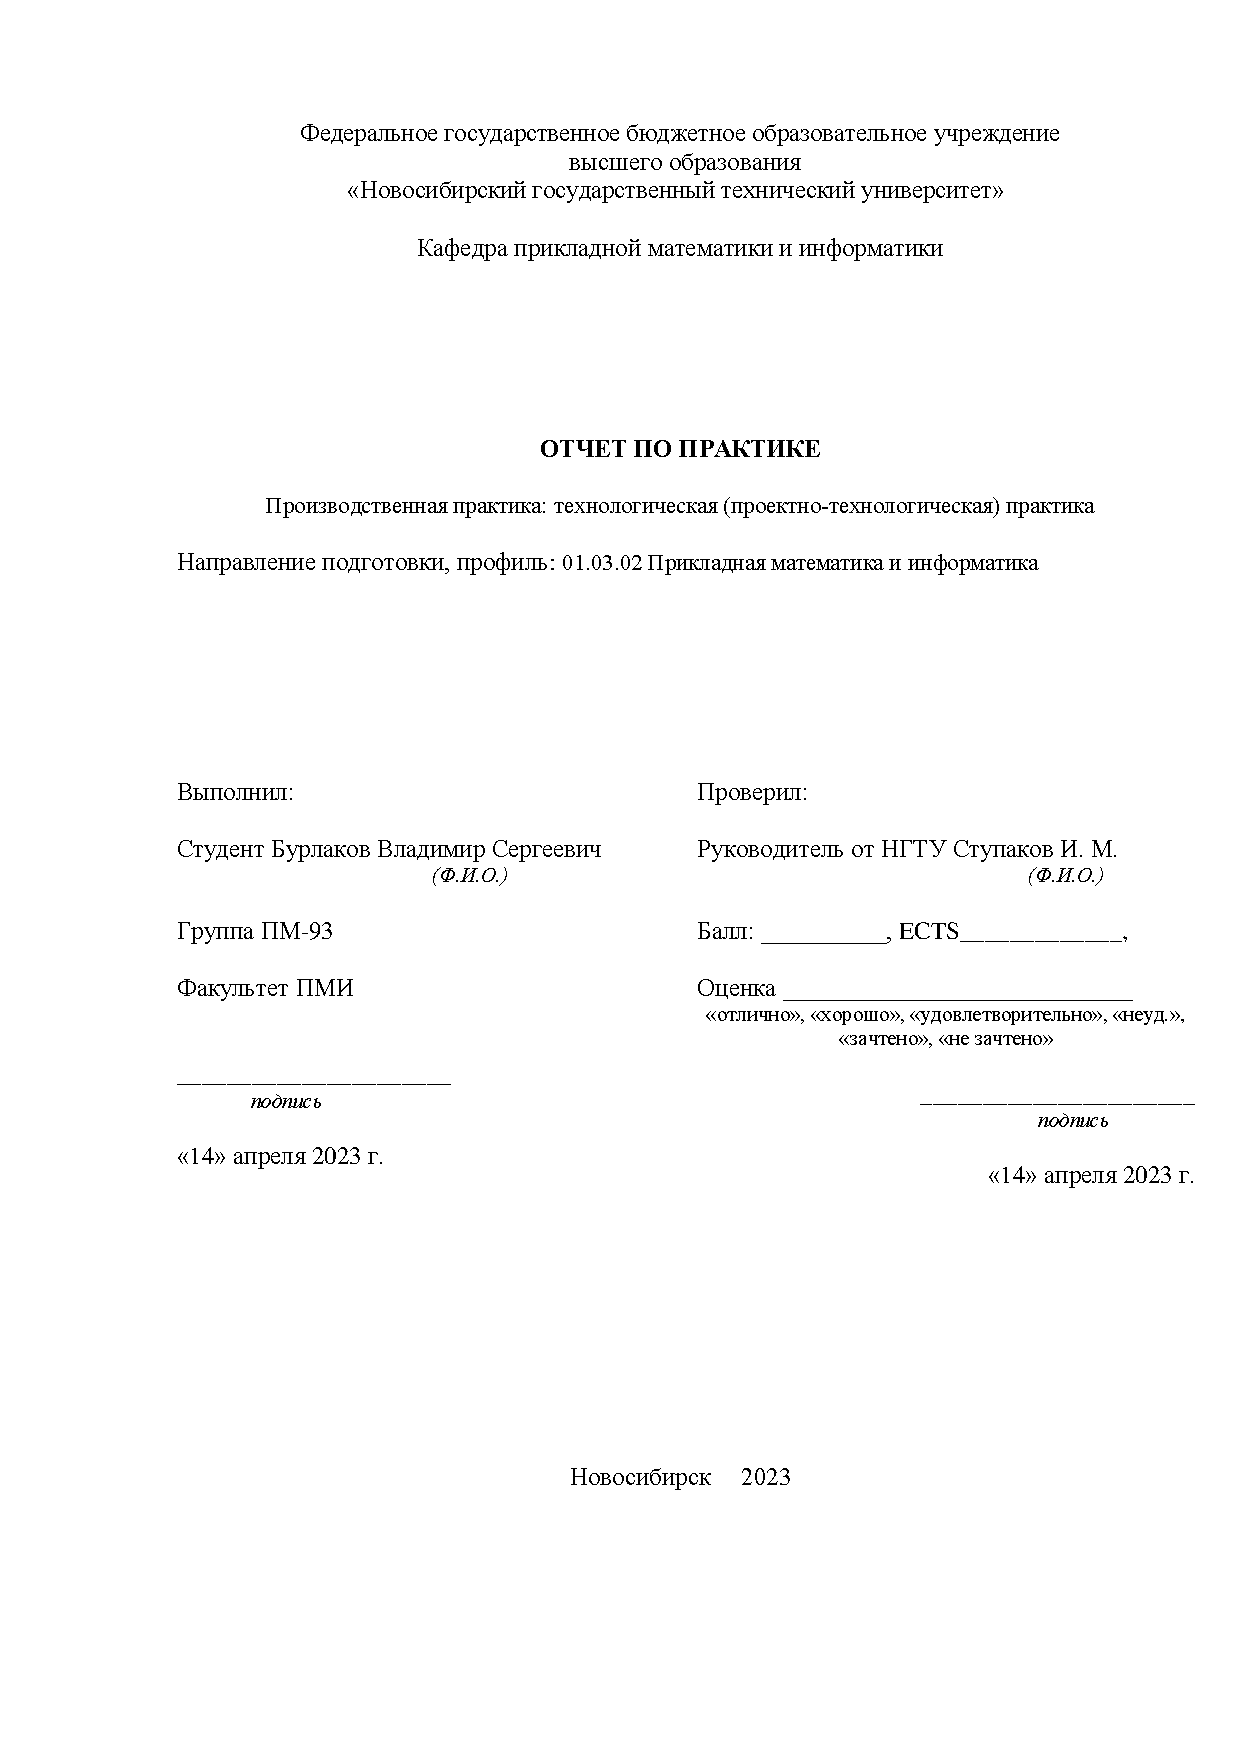
\includepdf{assets/title.pdf} % Титульный лист

\tableofcontents                          % Оглавление
\addtocontents{toc}{\protect\thispagestyle{empty}}
\thispagestyle{empty}

\addchap{ВВЕДЕНИЕ}
% FROM FIRST PRACTICE
% В современных условиях растущей автоматизации взаимодействия человека с компьютером, создание эффективных диалоговых систем остается одним из важных направлений развития искусственного интеллекта. Такие технологии могут помочь во многих индустриях, в том числе игровой индустрии. Новейшие технологии, использующие глубокое обучение, позволяют создавать диалоговые модели, которые способны эффективно обрабатывать естественный язык и предоставлять пользователю качественные ответы на запросы. Для эффективного обучения диалоговых моделей необходимо обладать качественным набором данных, содержащим диалоги между участниками. В данной работе было решено расширить концепцию диалогового датасета путем включения описания личности участников разговора. Это имеет большое значение при использовании в игровой индустрии.В данном отчете рассматривается процесс создания и анализа датасета DNDD (Dungeon \& Dragons Dialogues) для обучения диалоговой модели, основанный на сборе и предобработке данных из различных источников.

Разработка диалоговых моделей является активно развивающейся областью машинного обучения. Использование таких моделей имеет широкий спектр применений, включая чат-ботов, системы FAQ, и различные другие системы, где взаимодействие с пользователем через естественный язык играет важную роль. В игровой индустрии диалоговые модели имеют особое значение, поскольку они способны создавать реалистичные и интерактивные диалоги с неигровыми персонажами, улучшая игровой опыт. Качественные диалоговые модели способны улучшить игровой опыт, создавая более привлекательные и погружающие виртуальные миры.

Целью данной работы является создание эффективной диалоговой модели, способную генерировать качественные ответы на основе образа неигрового персонажа и контекста диалога, обеспечивая более реалистичные и интерактивные диалоги с неигровыми персонажами, на основе датасета DNDD (Dungeon \& Dragons Dialogues), специально созданного для данного исследования. В данной работе рассматриваются подготовка датасета для обучения модели, формулирование задачи для моделирования, поиск оптимальной модели и параметров, необходимых для успешного и эффективного обучения. % Введение

\chapter{ОСНОВЫ РАЗРАБОТКИ МОДЕЛЕЙ ИСКУССТВЕННЫХ НЕЙРОННЫХ СЕТЕЙ ДЛЯ ДИАЛОГОВЫХ ПРИЛОЖЕНИЙ}
\section{ВВЕДЕНИЕ В ИСКУССТВЕННЫЕ НЕЙРОННЫЕ СЕТИ}
Обработка естественного языка является крайне тяжелой задачей для моделирования стандартными алгоритмами. Машинное обучение позволяет решать задачи на основе статистических наблюдений из данных без явной алгоритмизации решения задачи. Недавние прорывы в области обработки естественного языка показывают, что методами машинного обучения можно частично или сполна выполнять многие человеческие задачи, например, краткое изложение текста, написание кода, общение с собеседником и другие, а также добиться результатов распознавания речи сопоставимых с результатами человека \cite{human-wer,whisper}.

Одним из основных аспектов машинного обучения является искусственная нейронная сеть (далее ИНС), созданная по подобию биологических нейронных сетей. Модель ИНС -- описание сети, математическая модель, часто представляемая в виде графа, нацеленная на решение задачи прогнозирования на основе обучающей выборки данных. Методами настройки параметров моделей под конкретную задачу называют методами обучения. Такими методами являются: обучение с учителем, обучение без учителя и обучение с подкреплением.

Каждый метод имеет свои особенности и применяется в зависимости от ситуации. Например, обычно обучение с учителем применяется в тех случаях, когда обучающий набор данных размечен на основе некоторых критериев. Такие задачи обычно являются задачами классификации, когда каждый экземпляр выборки имеет один или больше собственный класс. Такой подход имеет ограничения: как правило количество размеченных данных значительно меньше общего количество данных. В ситуациях, когда данные не размечены, применяется обучение без учителя. Благодаря такому подходу, можно обучить модель делить данные на кластеры, генерировать текст, изображения и т.д. Когда модели приходится принимать решения как интеллектуальный агент в условиях данной ей среды и соотвествующих откликов среды на решения, применяется метод обучения с подкреплением. Для построения мощных современных цифровых ассистенов могут использоваться все три подхода к обучению моделей, используя модели, полученных конкретным методом, в качестве промежуточных или вспомогательных, для обучения конечной модели \cite{state-of-gpt}.

\subsection{УСТРОЙСТВО ПРОСТОЙ ИСКУССТВЕННОЙ НЕЙРОННОЙ СЕТИ}

Устройство простой ИНС можно описать как взвешенный набор узлов, разделенный на слои, соединенные между собой активационными функциями $\varphi$. Функциям активации желательно иметь свойства: нелинейность, непрерывная дифференцируемость, бесконечная область значений, монотонность. При построении модели ИНС в качестве активационных функций часто используется одна из следующих функций:
\begin{enumerate}
    \item Гиперболический тангенс:
          \begin{equation}
              \varphi(z) = \frac{e^{2z}-1}{e^{2z}+1}.
          \end{equation}
    \item Функция ReLU:
          \begin{equation}
              \varphi(z) = \max(0, z).
              \label{relu}
          \end{equation}
    \item Функция GELU:
          \begin{equation}
              \varphi(z) = \frac{1}{2}z\left[1+\text{erf}\left({z}/\sqrt{2}\right)\right].
              \label{gelu}
          \end{equation}
    \item Логистическая функция (сигмоида):
          \begin{equation}
              \varphi(z) = \frac{1}{1+e^{-z}}.
          \end{equation}
    \item Многопеременная логистическая функция (softmax):
          \begin{equation}
              \varphi(z)_i = \frac{e^{z_i}}{\sum_{i=1}^{K}e^{z_j}}.
          \end{equation}
\end{enumerate}

Архитектуры ИНС могут сильно отличаться друг от друга в зависимости от поставленных задач и требований к качеству предсказаний модели. Раздел, который занимается изучением ИНС с большим количеством скрытых слоев, т.е. тех слоев, которые находятся между входным и выходным, называется глубоким обучением, а такие модели называются глубокими. Примером такой архитектуры модели может служить  трансформер \cite{transformer-paper}, речь о котором пойдет дальше.

Набор весов $W$ и отклонений $b$ являются параметрами модели, обозначаемые как $\theta$. Прогноз или функция гипотезы модели ИНС обозначается как $h_{\theta}$. $W^{[l]}$, $b^{[l]}$, $h_{\theta}^{[l]}$ -- веса, отклонения и выход модели на $l$-ом слое. Описать работу обобщенной модели ИНС c $L$ слоями можно следующим образом:
\begin{enumerate}
    \item $h_{\theta}^{[0]} = x$.
    \item $h_{\theta}^{[l]} = \varphi \circ \left(W^{[l-1]}h_{\theta}^{[l-1]}(x) + b^{[l-1]}\right), \text{где } 1 \le l \le L-1$.
    \item $h_{\theta} = h_{\theta}^{[L]} = W^{[L-1]}h_{\theta}^{[L-1]}(x) + b^{[L-1]}$.
\end{enumerate}

Примером простой ИНС может являться однослойный перцептрон. Схема однослойного перцептрона представлена на рис. \ref{fig:perceptron}.

\begin{figure}[H]
    \centering
    \begin{tikzpicture}[
            init/.style={
                    draw,
                    circle,
                    inner sep=2pt,
                    font=\Huge,
                    join = by -latex
                },
            squa/.style={
                    draw,
                    inner sep=2pt,
                    font=\Large,
                    join = by -latex
                },
            start chain=2,node distance=17mm
        ]
        \node[on chain=2]
        (x2) {$x_2$};
        \node[on chain=2,join=by o-latex]
        {$w_2$};
        \node[on chain=2,init] (sigma)
        {$\displaystyle\Sigma$};
        \node[on chain=2,squa,label=above:{\parbox{2cm}{\centering Функция \\ активации}}]
        {$\varphi$};
        \node[on chain=2,label=above:Выход,join=by -latex]
        {$y$};
        \begin{scope}[start chain=1]
            \node[on chain=1] at (0,1.5cm)
            (x1) {$x_1$};
            \node[on chain=1,join=by o-latex]
            (w1) {$w_1$};
        \end{scope}
        \begin{scope}[start chain=3]
            \node[on chain=3] at (0,-1.5cm)
            (x3) {$x_3$};
            \node[on chain=3,label=below:Веса,join=by o-latex]
            (w3) {$w_3$};
        \end{scope}
        \node[label=above:\parbox{2cm}{\centering Отклонение\\$b$}] at (sigma|-w1) (b) {};

        \draw[-latex] (w1) -- (sigma);
        \draw[-latex] (w3) -- (sigma);
        \draw[o-latex] (b) -- (sigma);

        \draw[decorate,decoration={brace,mirror}] (x1.north west) -- node[left=10pt] {Вход} (x3.south west);
    \end{tikzpicture}
    \caption{Однослойный перцептрон}
    \label{fig:perceptron}
\end{figure}

\subsection{ОБУЧЕНИЕ С УЧИТЕЛЕМ ИСКУССТВЕННОЙ НЕЙРОННОЙ СЕТИ}

Как было сказано раннее, для того, чтобы обучить ИНС с учителем, требуется иметь такой набор данных, где каждый элемент имел соответствующую метку класса. Элементы набора данных, т.е. входные данные, принадлежат некоторому входному пространству $\mathcal{X}$, например, картинкам кошек, а метки принадлежат к выходному пространству $\mathcal{Y}$, например, породе кошек. Из такого набора данных $\mathcal{D}$ мы строим тренировочную подвыборку, состоящую из пар, элементов:

\begin{equation}
    \mathcal{D}_{\text{train}} = \{\,(x_i, \hat y_i) \mid x_i \in \mathcal{X}, \hat y_i \in \mathcal{Y}, i=\overline{1, \dots, n}, n \le \lvert \mathcal{D} \rvert\,\}.
\end{equation}

Мы стремимся получить целевую функцию ИНС $h_{\theta^*}$ с оптимальным набором параметров $\theta^*$ на основе $\mathcal{D}_{\text{train}}$, при котором $h_{\theta^*}$ наиболее эффективно отображает из пространства $\mathcal{X}$ в пространство $\mathcal{Y}$. Для определения того, насколько эффективно предсказывает модель, требуется иметь неотрицательную функцию $\ell: \mathcal{Y} \times \mathcal{Y} \rightarrow \mathbb{R}^+$, которая измеряет ошибку предсказания $h_{\theta}(x)$ по отношению к истинной метке $\hat y$. Такие функции, как правило, называются функциями ошибки или функциями потерь. Функция потерь выбирается исходя из условий конкретной задачи, но часто является одной из следующих функций:
\begin{enumerate}
    \item Функция потерь $L_1$:
          \begin{equation}
              \ell\left(h_\theta(x), \hat y\right) = \lvert \hat y - h_\theta(x) \rvert.
          \end{equation}
    \item Функция потерь $L_2$:
          \begin{equation}
              \ell\left(h_\theta(x), \hat y\right) = \big(\hat y - h_\theta(x)\big)^2.
          \end{equation}
    \item Функция потерь перекрестной энтропии:
          \begin{equation}
              \ell\left(h_\theta(x), \hat y\right) = - \hat y\log{h_\theta(x)}.
          \end{equation}
    \item Функция потерь NLL:
          \begin{equation}
              \ell\left(h_\theta(x), \hat y\right) = -\left[\hat y \log{h_\theta(x)} + (1 - \hat y)\log(1 - h_\theta(x))\right].
          \end{equation}
\end{enumerate}

Обучение модели с учителем сводится к задаче минимизации функции потерь по тренировочной выборке:

\begin{equation}
    \mathcal{L}_{\mathcal{D}_{\text{train}}}(\theta) = \frac{1}{\lvert \mathcal{D}_{\text{train}} \rvert}\sum_{i=1}^{\lvert \mathcal{D}_{\text{train}} \rvert}\ell(h_{\theta}(x_i),\hat y_i) \rightarrow \min_{\theta}.
\end{equation}

Чтобы решить такую задачу минимизации функции потерь по тренировочной выборке, требуется вычислить:

\begin{equation}
    \frac{\partial \mathcal{L}_{\mathcal{D}_{\text{train}}}(\theta)}{\partial \theta}.
    \label{loss-grad}
\end{equation}

Метод, который позволяет аналитически вычислить градиент (\ref{loss-grad}) в точке, называется методом обратного распостранения ошибки \cite{backprop-theory}. Основа метода -- автоматическое построение графа вычислений и правило вычисления производной сложной функции. С полученным градиентом функции потерь параметры модели ИНС меняются алгоритмом оптимизации. Одними из важных составляющих алгоритмов оптимизации являются выбор размера шага оптимизатора $\eta$, называемым еще скоростью обучения, и планировщик скорости обучения $\varsigma$, поскольку влияют на скорость процесса обучения и на преодоления методом оптимизации локальных минимумов. Частым выбором таких алгоритмов являются: <<\textit{GD}>> (градиентный спуск), <<\textit{SGD}>> (стохастический градиентный спуск), Adam, AdaFactor \cite{optimizers-paper,adafactor-paper}.

Обучение является итеративным процессом, где итерация или шаг итерации -- это обработка моделью одного или нескольких примеров обучающей выборки. Обработка полного набора выборки называют эпохой.

Алгоритм обучения модели ИНС с учителем представлен ниже.

\begin{algorithm}
    \floatname{algorithm}{Алгоритм}
    \caption{Обучение модели ИНС с учителем}
    \begin{algorithmic}[1]
        \State Инициализировать $\theta$ случайно или по некоторому закону распределения.
        \State По каждой эпохе из количества эпох:
        \State\hspace{\algorithmicindent} По каждому примеру $(x, \hat y)$ из обучающей выборки $\mathcal{D}_{\text{train}}$:
        \State\hspace{\algorithmicindent}\hspace{\algorithmicindent} Получить предсказание модели $y \gets h_{\theta}(x)$.
        \State\hspace{\algorithmicindent}\hspace{\algorithmicindent} Получить значение функции потерь $\ell(y, \hat y)$.
        \State\hspace{\algorithmicindent}\hspace{\algorithmicindent} Получить градиент $\nabla \ell$ методом обратного распостранения.
        \State\hspace{\algorithmicindent}\hspace{\algorithmicindent} Сделать шаг оптимизации.
        \State\hspace{\algorithmicindent}\hspace{\algorithmicindent} Аккумулировать значение общей функции потерь $\mathcal{L} \gets \mathcal{L} + \ell(y, \hat y)$.
    \end{algorithmic}
\end{algorithm}

Однако одной тренировочной подвыборки чаще всего не достаточно для успешного обучения модели. Как правило используют три подвыборки исходных данных $\mathcal{D}$. Помимо обучающей, используется валидационная $\mathcal{D}_{\text{val}}$, которая используется в конце эпохи обучения, на которой модель не обучается, но проверяется на наборе данных, которые она не видела, для корректировки гиперпараметров модели. Гиперпараметры -- это параметры, которые используются для контроля процесса обучения. Примерами гиперпараметров могут служить как вышеупомянутые $\eta$ и $\varsigma$, так и количество слоев в модели, активационные функции и т.д. Для оценки итогого качества модели обычно используется тестовая выборка $\mathcal{D}_{\text{test}}$. Методы, которые разбивают исходный набор данных $\mathcal{D}$ на подвыборки, называются методами стратификации.

Хоть $\ell$, $\mathcal{L}$ и показывают качество прогнозирования модели $h_{\theta}$, но на практике анализировать качество модели только по значениям функции потерь -- это сложная задача. Помимо функции потерь используются метрики оценки прогнозирования. Выбор метрик сильно зависит от поставленной задачи.

\section{ВЕКТОРНОЕ ПРЕДСТАВЛЕНИЕ ТЕКСТА}
Из устройства работы ИНС следует, чтобы данные, на которых обучается модель были численными. Поэтому при обработке текста требуется получить его векторное представление для дальнейшей работы с ним.

Простейшим методом представления слов в векторном пространстве является <<\textit{One-Hot Encoding}>> (быстрое кодирование). Его суть заключается в присвоении каждому слову из входной последовательности слов вектора, где в позиции, соотвествующей слову в словаре размерностью словаря, ставится единица, а во всех остальных позициях -- ноль. Словарь содержит весь список возможных слов для кодирования. Размерность такого вектора составляет $1 \times N$, где $N$ -- количество слов в словаре. Пример быстрого кодирования показан ниже.

\begin{table}[H]
    \captionsetup{format=hang, singlelinecheck=false}
    \raggedleft
    \caption{Пример словаря}
    \label{tab:dict}
    \centering
    \begin{tabular}{|p{5cm}|}
        \hline
        \textbf{Цвет} \\
        \hline
        Красный       \\
        \hline
        Зеленый       \\
        \hline
        Синий         \\
        \hline
    \end{tabular}
\end{table}

\begin{table}[H]
    \captionsetup{format=hang, singlelinecheck=false}
    \raggedleft
    \caption{Пример быстрого кодирования}
    \label{tab:ohe}
    \centering
    \begin{tabular}{|p{5cm}|p{5cm}|p{5cm}|}
        \hline
        \textbf{Красный} & \textbf{Зеленый} & \textbf{Синий} \\
        \hline
        1                & 0                & 0              \\
        \hline
        0                & 1                & 0              \\
        \hline
        0                & 0                & 1              \\
        \hline
    \end{tabular}
\end{table}

Представлением текстовых данных в численном виде могут заниматься и модели ИНС: учить полезную информацию о входной последовательности, сжато представлять текст в векторном пространстве, решая задачу языкового моделирования, для последующего использования этого представление на конечной задаче, например, задаче классификации или задаче генерации текста. Одной из первых широко распостраненных обученных моделей для кодирования текста является Word2vec \cite{word2vec-paper}.

В современных моделях для обработки естественного языка в качестве основы векторного представления данных используют метод, называемый токенизацией. Токенизация -- разбиение входного текста на части, называемые токенами. В качестве части текста могут быть как слова целиком, так и части слов. Токенизация представляет входной текст как вектор, состоящий из номеров токенов в общем словаре. Размер закодированной последовательности может зависеть как длиной входной последовательности, так и от требуемой длины, дополняя неиспользуемое пространство специальными токенами. Пример токенизации <<\textit{Byte-Pair Encoding}>> (побайтное кодирование) \cite{bpe-paper} для входной последовательности <<Many words map to one token, but some don't: indivisible. Sequences of characters commonly found next to each other may be grouped together: 1234567890>> представлен ниже. Токены, на которые разбивает токенизитор входную последовательность, показаны на рис. \ref{fig:tok-viz-words-fig}.
\begin{figure}[H]
    \centering
    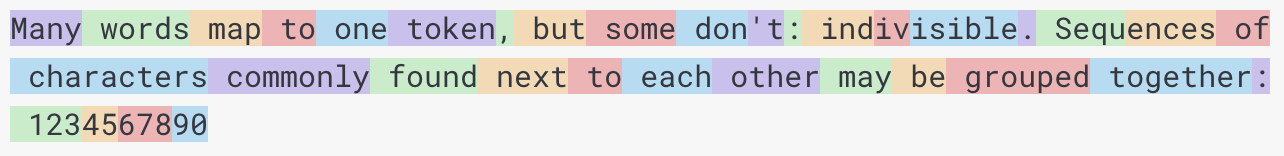
\includegraphics[width=\textwidth]{tok-viz-words-fig}
    \caption{Пример работы токенизации}
    \label{fig:tok-viz-words-fig}
\end{figure}

Векторное представление такой последовательность токенов показано на рис. \ref{fig:tok-vec}.
\begin{figure}[H]
    \centering
    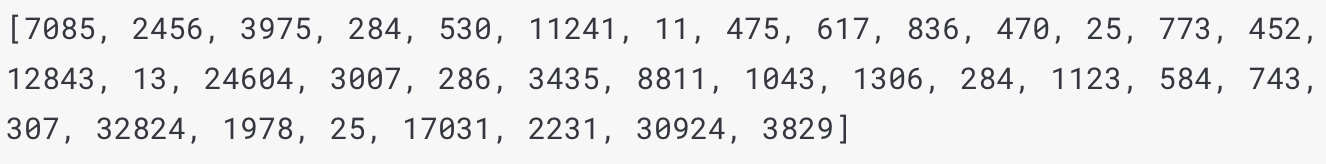
\includegraphics[width=\textwidth]{tok-vec}
    \caption{Векторное представление токенов}
    \label{fig:tok-vec}
\end{figure}

\section{АРХИТЕКТУРА ТРАНСФОРМЕР}
Стандартным выбором архитектуры модели ИНС при обработке естественного языка является архитектура трансформер. Одними из первых моделей, созданных на базе данной архитектуры, стали GPT \cite{gpt-paper}, T5 \cite{t5-paper} и BERT \cite{bert-paper}. Трансформер состоит из набора блоков <<\textit{encoder}>> (кодировщика) и <<\textit{decoder}>> (декодировщика).

Для начала происходит токенизация входного текста, а затем полученное векторное представление токенов дополняется позициональным кодированием, чтобы учитывать информацию о позиции токена во входном тексте.

Далее полученное векторное состояние передается на $N$ идущих друг за другом блоков кодировщика. Каждый блок кодировщика состоит из двух главных компонент: механизм <<\textit{Self-Attention}>> (самовнимание) и сети прямого распостранения (обобщенная версия сети, показаной на рис. \ref{fig:perceptron}). После прохождения $N$ блоков кодировщика, векторное состояние передается к $N$ блокам декодировщика.

В свою очередь каждый блок декодировщика схож с устройством блока кодировщика с добавлением <<\textit{Cross-Attention}>> (перекресного внимания) от векторного представления состояния кодировщика. Полную версию архитектуры трансформер можно наблюдать на рис. \ref{fig:transformer-arch}.
\begin{figure}[H]
    \centering
    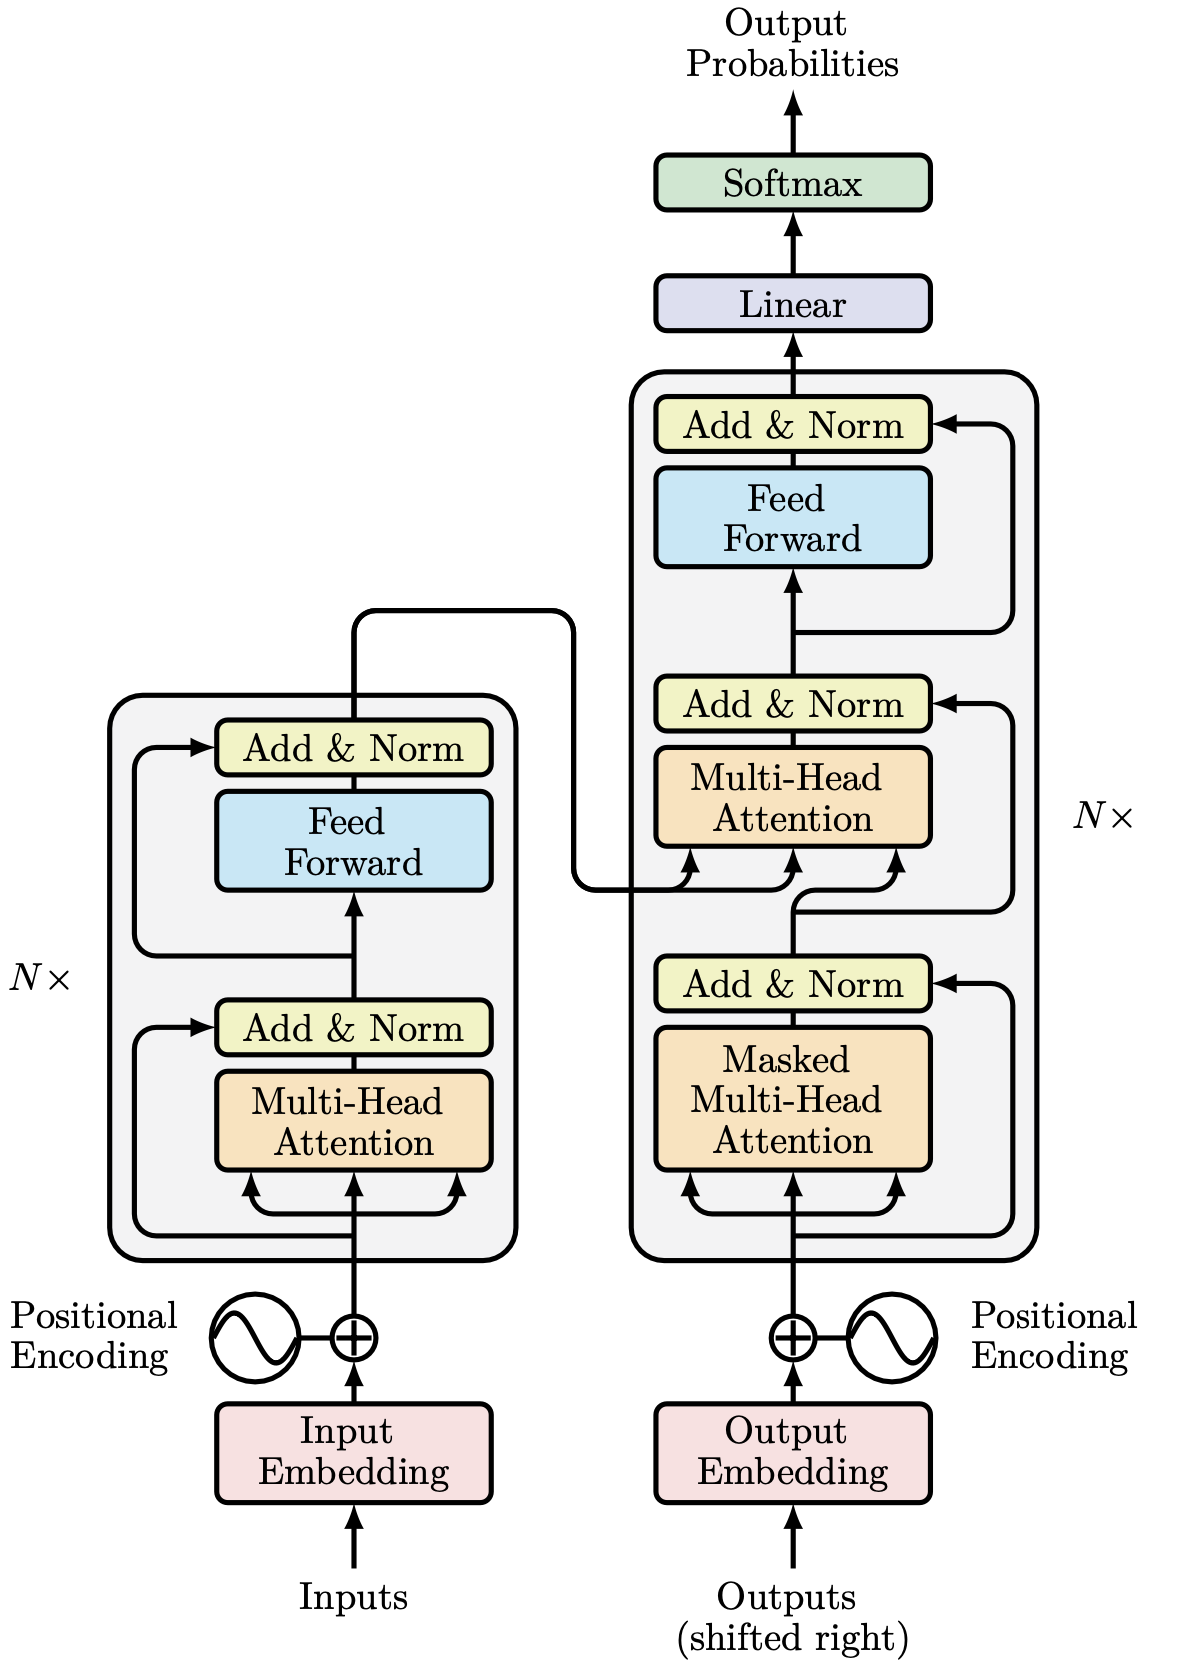
\includegraphics[width=0.4\textwidth]{transformer-arch}
    \caption{Архитектура трансформер}
    \label{fig:transformer-arch}
\end{figure}
\subsection{МЕХАНИЗМ ВНИМАНИЯ}
Механизм внимания -- ключевой механизм в архитектуре трансформер. Его суть заключается в учитывании взаимодействия элемента входной последовательности со всеми другими элементами. Таким образом, модель может фокусироваться на более важных частях данных, даже если такая информация содержится в небольшой части данных.

Разберем более подбробно этот механизм. Входное векторное состояние данных представляется как набор трех главных компонент внимания: <<\textit{query}>> (запрос), <<\textit{keys}>> (ключи) и <<\textit{values}>> (значения). Преставление входных данных осуществляется за счет проекции входного векторного состояния $I$ на пространства этих компонент, т.е.:

\begin{enumerate}
    \item $Q = I \cdot W_Q^T$.
    \item $K = I \cdot W_K^T$.
    \item $V = I \cdot W_V^T$.
\end{enumerate}

Из полученных векторов вычисляем результирующий вектор:

\begin{equation}
    \text{Attention}\left(Q,K,V\right) = \text{softmax}\left(\frac{QK^T}{\sqrt{d_k}}\right)V\text{, где }d_k = \dim(K).
    \label{eq:attn}
\end{equation}

Проинтерпретировать формулу \ref{eq:attn} можно следующим образом:

\begin{enumerate}
    \item Запрос $Q$ проектируется в пространство ключей $K$, т.е. получаем матрицу: $S = QK^T$.
    \item Для запроса $Q$ в смаштабированном пространстве $K$ ищется наиболее подходящие, т.е. близкие ключи: $A=\text{softmax}\left(\frac{S}{\sqrt{d_k}}\right)$.
    \item Затем полученная матрица умножается на искомые значения, получая взвешенную сумму входного векторного состояния: $O=AV$.
\end{enumerate}

Важно отметить, что матрицы внутренного состояния $W_Q,W_K,W_V$ -- обучаемые параметры.

В случае, когда $Q, K, V$ получаются из одного внутреннего состояния, такой вид механизма внимания называется самовнимание. Если $K, V$ получены как выход внутреннего состояния кодировщика, а $Q$ получен как внутренне состояние декодировщика, то такой вид внимания называется перекресным вниманием. Такой механизм позволяет модели учитывать взаимодействие между элементами входной и выходной последовательностей. Таким образом, блоки декодировщика могут использовать информацию из блоков кодировщика для генерации правильных элементов выходной последовательности.

Также может потребоваться, чтобы модель оперировала векторным состоянием входного текста до позииции текущего токена. Чтобы закрыть доступ модели к такого рода информации, применяется маскированное внимание.

Вместо вычисления одного внимания с размерностью $d_{\text{model}}$, можно вычислять внимание c фокусом на разные участки входной последовательности параллельно. Такое внимание называется <<\textit{Multi-Head Attention}>> (многоголовое внимание) и вычисляется как:

\begin{equation}
    \text{MHA}(Q, K, V) = \text{Concat}(\text{head}_1, \dots, \text{head}_h) W^O,
\end{equation}

где $\text{head}_i = \text{Attention}(QW_i^Q, KW_i^K, VW_i^V)$.

Благодаря тому, что операции перемножения матриц -- высокооптизируемые операции, данный механизм эффективен с точки зрения производительности.

\subsection{МОДЕЛЬ T5: АРХИТЕКТУРА И ЕЕ ОСОБЕННОСТИ}
Обучение модели архитектуры трансформер обычно происходит в два этапа. Сначала модель обучается решать задачу языкового моделирования на огромном наборе неразмеченных данных. Такой процесс крайне затратен, т.к. требует больших мощностей и огромного набора данных. Такой этап называется <<\textit{pretrain}>> (предварительное обучение), после чего модель дообучают на конкретной задаче, например, на генерации текста или на задаче поддержания диалога, на меньшем, но размеченном наборе данных. Этап дообучения значительно менее затратен, чем предварительное обучение.

Модель <<\textit{Text-To-Text Transfer Transformer}>> (T5) -- это модель глубокого обучения, использующая архитектуру трансформер, разработанная компанией Google для решения многих различных задач обработки естественного языка. Преимущества данной модели является универсальность: Т5 изначально была обучена на задачах перевода, кратком изложении текста, классификации текста и на ответа на вопрос, разделяя задачи специальным префиксом. Одной из особенностей моделей T5 является их способность работать с разными типами входных и выходных данных. Например, модель может обрабатывать текстовые данные различных длин и форматов, а также генерировать тексты различных стилей и тематик. В качестве токенизатора T5 использует SentencePiece \cite{sentencepiece-paper}.

Предварительное обучение Т5 производилось на наборе данных <<\textit{Colossal Clean Crawled Corpus}>> (C4), содержащий 356 миллиардов токенов, занимающий 750 гигабайт дискового пространства, на задаче <<\textit{Masked Language Modeling}>> (моделирование замаскированного языка). Задача заключается в востановлении исходного текста на основе <<поврежденного>> текста, где <<повреждалось>> 15\% токенов, в которых 90\% заменялось на специальный токен \texttt{[MASK]}, а остальные 10\% заменялись на случайный токен из словаря.

После предварительного обучения модель дообучили на конечных задачах, описанных выше. Со временем набор изначальных задач расширили набором задач, состоящим из инструкций на понимание и генерацию текста на естественном языка, что значительно улучшило качество модели для последующего обучения, например, на задаче поддержания диалога \cite{flan-paper}.

\section{ПОСТАНОВКА ЗАДАЧИ ДИАЛОГОВОЙ СИСТЕМЫ}
Эмуляция диалога, обучение диалоговых агентов или чат-ботов относятся к области генерации и классификации текста. Такие модели должны эффективно обрабатывать естественный язык и формировать ответы в рамках диалога. В качестве диалоговой системы может выступать не одна модель ИНС. Различные задачи, например, классификации, генерации текста и автоматичского распознавания речи могут выполнять разные модели. Разберем основные компоненты диалога:

\begin{enumerate}
    \item Состояние диалога: Диалоговая система должна понимать намерения запроса пользователя и те сущности, которые фигурируют в запросе. Намерением пользователя может быть покупка, а сущностью -- товар. Такие задачи являются задачами классификации.
    \item Контекст диалога: диалоговая система должен учитывать контекст предыдущих сообщений, чтобы дать более точный и подходящий ответ.
    \item Цель диалога: диалоговая система может иметь цель, которую она преследует в рамках диалога. Такой целью может быть, например, имитация поведения неигрового персонажа.
    \item Шаг диалога: одна итерация в обмене сообщениями между пользователем и диалоговой системой. Каждый шаг диалога представляет собой один вопрос или одно сообщение от системы, на которое пользователь должен ответить. Затем система обрабатывает ответ пользователя и переходит к следующему шагу диалога. Шаги диалога помогают упорядочить и структурировать обмен сообщениями между пользователем и диалоговой системой. Пример шагов диалога приведет в таблице \ref{tab:dialogue-turn}.
\end{enumerate}

\begin{table}[H]
    \captionsetup{format=hang, singlelinecheck=false}
    \raggedleft
    \caption{Пример диалоговых шагов}
    \label{tab:dialogue-turn}
    \centering
    \begin{tabular}{|p{5cm}|p{10cm}|}
        \hline
        Шаг 1 & Система: Здравствуйте, чем я могу Вам помочь?            \\
        \hline
        Шаг 2 & Пользователь: Добрый день, я хочу заказать пиццу на дом. \\
        \hline
        Шаг 3 & Система: Какой размер пиццы Вы хотели бы заказать?       \\
        \hline
    \end{tabular}
\end{table}

Для обучения диалоговых моделей, способных продолжить диалог, требуется набор данных, содержащий диалоги. Такую задачу можно решить обучением с учителем. Для этого необходимые компоненты диалога должны быть в формате $(x, \hat y)$, где в качестве $x$ выступает строка, содержащая цель диалога и его контекст, а в качестве $\hat y$ выступает желаемый ответ диалоговой модели.

\chapter{ОПИСАНИЕ РАЗРАБОТАННЫХ ПРОГРАММ}
Язык программирования Python \cite{python-lang-site} является стандартным выбором языка для разработки и обучения моделей ИНС благодаря богатой экосистеме пакетов. Сами пакеты для разработки моделей ИНС могут быть написаны на более низкоуровневом языке программирования, например, на C++ \cite{cpp-docs} с использованием CUDA \cite{cuda-docs} для высокой производительности кода, в то время как пакет, которым пользуется разработчик, доступен в качестве интерфейса на языке Python для высокой производительности разработчика. Исходя из этого, выбором языка, на котором написаны алгоритмы обработки набора данных DNDD, поиска оптимильных параметров и обучения модели является Python.

\section{ОБРАБОТЧИК НАБОРА ДАННЫХ DNDD}
Обработчик набора данных DNDD доступен как приложение командной строки, полный код которого показан в приложении \ref{app:code}. Параметры обработчика:
\begin{enumerate}
    \item Подмножество игр, которые будут обрабатываться приложением указывается как аргумент командной строки \texttt{--subsets}. Если ведется обработка полного набора данных, то этот аргумент можно опустить или присвоить ему значение \texttt{all}.
    \item Сгенерировать описания неигровых персонажей (далее NPC) можно аргументом \texttt{--generate\_descriptions}. В таком случае необходимо либо иметь доступ к серверу с языковой моделью, либо предварительно запустить сервер самостоятельно, используя например простой интерфейс от Gradio \cite{gradio-docs}. В любом случае желательно передать URL на эндпоинт, где доступна языковая модель, аргументом \texttt{--model\_server\_url}. При отсутствии такого аргумента, URL по умолчанию будет \url{http://127.0.0.1:7860}.
    \item Если список описаний NPC уже есть, то его можно передать в приложение через аргумент \texttt{--description\_file}.
    \item В случае, если требуется, чтобы приложение сохранило работу обработанного набора данных, который готов к конечному использованию для обучения модели, тогда используется аргумент \texttt{--build-final}. Если требуется органичить максимальное количество диалогов NPC, тогда следует использовать аргумент \texttt{--limit\_dialogues}.
\end{enumerate}

При разработке приложения для обработки набора данных DNDD были использованы следующие Python пакеты и библиотеки:
\begin{itemize}
    \item Argparse, встроенная в язык Python библиотека создания программ командной строки.
    \item Tqdm \cite{tqdm-docs} для визуализации прогресса работы приложения.
    \item Requests, встроенная в язык Python библиотека запросов, для доступа к языковой модели через REST <<\textit{Application Programming Interface}>> (API).
    \item Datasets \cite{hf-datasets-docs} для сериализации и хранения обработанного набора данных и объекта, который используется как набор данных при обучении модели.
    \item Transformers \cite{transformers-docs} для оценки количества токенов отправляемых данных в модель для генерации описаний.
    \item Pandas \cite{pandas-docs} для внутренней обработки набора данных.
    \item Os, встроенная в язык Python библиотека взаимодействия с операционной системой, для работы с файлами.
    \item Json, встроенная в язык Python библиотека взаимодействия с JSON файлами, для десериализации исходных данных.
\end{itemize}

\section{МОДУЛИ ОБУЧЕНИЯ И ПОИСКА ОПТИМАЛЬНЫХ ГИПЕРПАРАМЕТРОВ}
Поиск оптимальных гиперпараметров и обучение модели реализованы через Python скрипты. Для обучения модели была использована библиотека Transformers, а для оптимизации процесса обучения и используемых вычислительных мощностей библиотека PEFT \cite{peft-docs}. Для загрузки подготовленных наборов данных используется библиотека Datasets, после чего токенизируется для дальнейшей работы. Для поиска оптимальных гиперпараметров класс sweep библиотеки Weights \& Biases \cite{wandb-docs} перебирает указанный набор.

\section{ДЕМО ПРИЛОЖЕНИЕ ДЛЯ СОЗДАНИЯ ДИАЛОГОВОЙ СИСТЕМЫ ДЛЯ РАЗРАБОТЧИКОВ ВИДЕОИГР}
В качестве демо приложения диалоговой системы было написано веб-приложение на фреймворке Gradio. В этом приложении можно создать NPC и пообщаться с ним через текстовый или аудио интерфейс. Приложение содержит модули автоматического распознавания речи, эмоциональной классификации речи, классификации намерений, семантического поиска и диалоговой модели. Доступ к приложению осуществляется как через REST API, так и через веб-интерфейс. На экране создания NPC можно заполнить поля, необходимые для описания NPC, и добавить NPC в список доступных для диалога. После создания NPC, на экране диалога можно выбрать конкретного NPC, с которым можно провести диалог. Экран создания NPC можно наблюдать на рис. \ref{demo-npc-creation}, а экран диалога на рис. \ref{demo-dialogue}.
\begin{figure}[H]
    \centering
    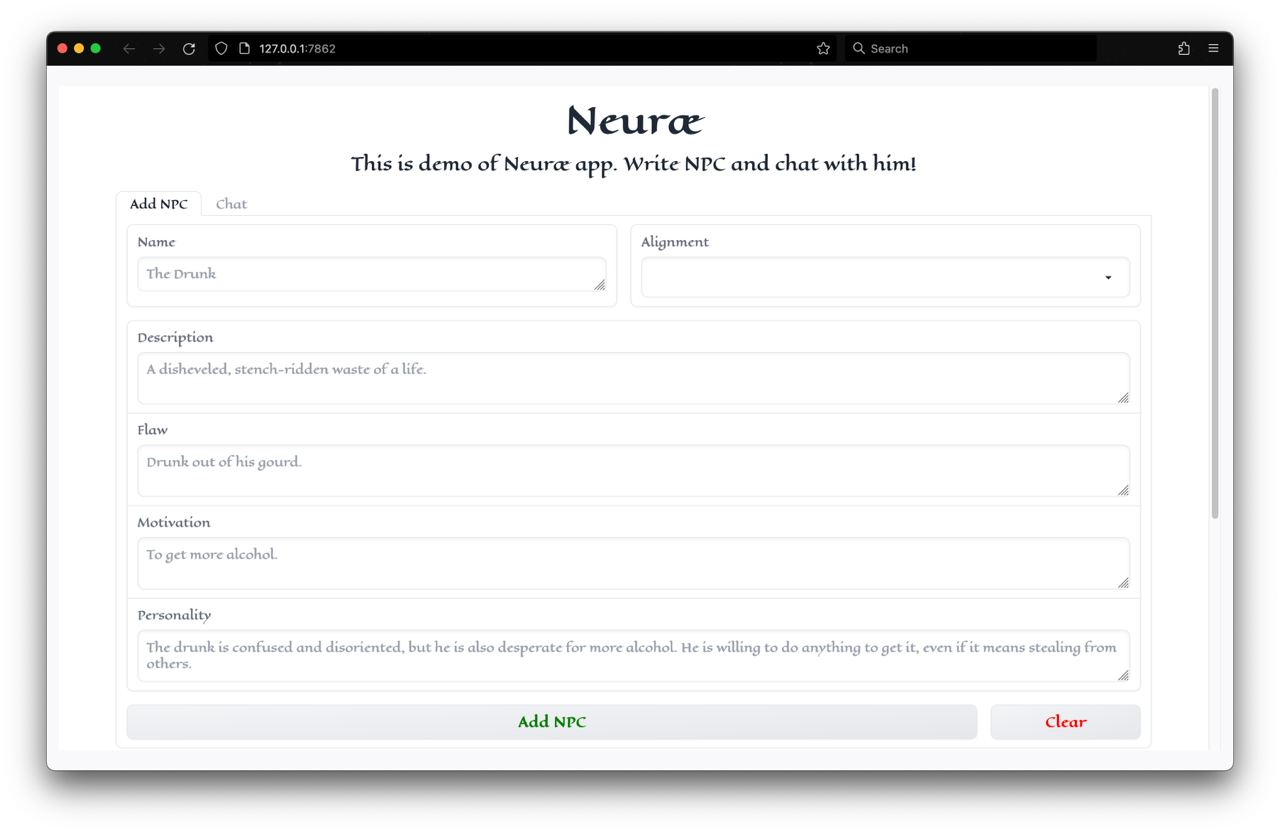
\includegraphics[width=1.\textwidth]{neurae-demo-npc-creation}
    \caption{Экран создания NPC}
    \label{demo-npc-creation}
\end{figure}
\begin{figure}[H]
    \centering
    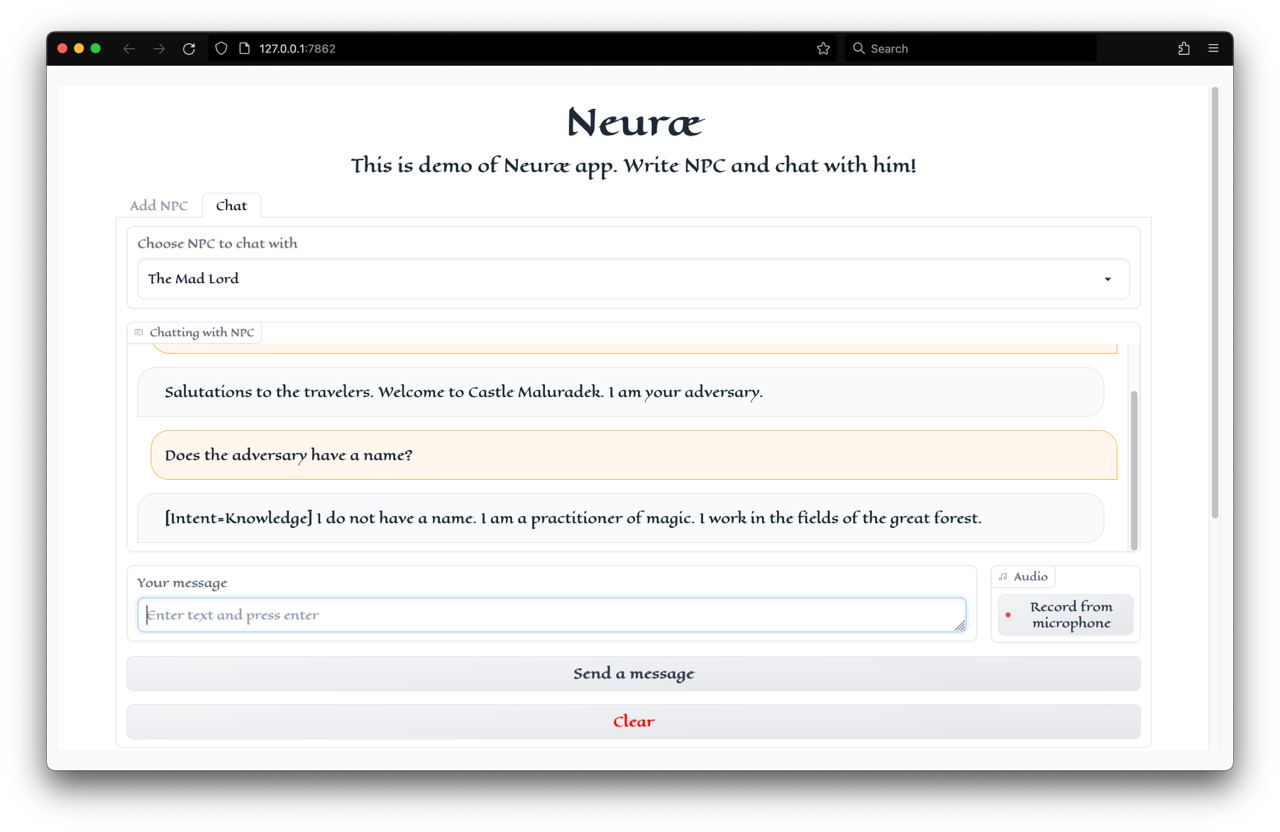
\includegraphics[width=1.\textwidth]{neurae-demo-dialogue}
    \caption{Экран диалога с NPC}
    \label{demo-dialogue}
\end{figure}

\chapter{РАЗРАБОТКА НАБОРА ДАННЫХ DNDD}
\section{СТРУКТУРА НАБОРА ДАННЫХ}
% TODO: Добавить больше описания в то, как получается датасет
Чтобы создать набор данных для обучения диалоговой модели, которая эмулирует поведение  неигровых персонажей (далее NPC) по заданному описанию в играх, необходимо иметь диалоги, построенные по определенной системе правил. Одной из самой распостраненной, обширной и гибкой системой правил, по которым можно описать NPC, является система Dungeon \& Dragons (далее D\&D), т.к. она обладает вполне определенной структурой. Например, персонажи обязаны иметь конкретное мировозрение, определяющее их поведение и взгляды на поступки, мотивацию, внешнее описание и слабости. Поэтому выбор такой системы выглядит естественным. 

Набор данных, созданный из данных игр во вселенной D\&D, должен содержать примеры диалогов NPC с главным героем и примеры описания NPC в формате Name/Alignment/Description/Flaw/Motivation/Personality.

\section{СБОР ДАННЫХ}
\subsection{СБОР И ПРЕДОБРАБОТКА ПЕРВОНАЧАЛЬНЫХ ДАННЫХ}
Первоначальные данные были получены из следующих игр: 
\begin{enumerate}
      \item <<Icewind Dale: Enhanced Edition>>.
      \item <<Planescape: Torment: Enhanced Edition>>.
\end{enumerate}

Такой выбор игр неслучаен: все эти игры были созданы с помощью  игрового движка Infinity Engine. Диалоги были получены следующим образом:
\begin{enumerate}
      \item Диалоги, которые были использованы, находились в скомпилированом файле, который можно было найти внутри <<.bif>> файла.
      \item Чтобы получить диалоги NPC в скомпилированном формате с расширением <<.dlg>>, была использована программа WinBif.
      \item Далее, с помощью WeiDU \cite{weidu-repo}, специального транслятора,
            написанного для создания собственных диалогов в играх Infinity Engine в качестве модификации, эти файлы были преобразованы в формат языка <<.d>>;.
      \item Наконец, конвертированы полученные файлы в удобный для анализа JSON-формат. Такие файлы содержат возможные диалоги NLP с главным героем.
\end{enumerate}

\subsection{ПОСТОБРАБОТКА ПЕРВОНАЧАЛЬНЫХ ДАННЫХ}

Для начала полученные JSON файлы были проанализированы на предмет NPC, т.к. в этих играх описания взаимодействия с неодушевленными предметами: порталами, сферами и т.д. Из-за того, что такие описания не содержат непосредственно диалогов, они были удалены из выборки. Также было замечено, что в игре <<Planescape: Torment: Enhanced Edition>> в отличии от остальных игр на движке Infinity Engine в диалоговых файлах (помимо самих диалогов) в текстовом виде достаточно часто было описано то, что видит перед собой игрок, что в последствии сильно поможет составлению набора данных. Такую полезную информацию нельзя упускать и следует иметь помимо обычных реплик NPC дополнительный констекст диалога. К тому же игра обладает самым большим размером корпуса диалогов среди игр во вселенной D\&D.

\chapter{ОБУЧЕНИЕ МОДЕЛЕЙ}
\section{ПОИСК ОПТИМАЛЬНОЙ МОДЕЛИ}
В области исследований генеративных моделей преобладание больших моделей привело к проблемам при проведении исследований и анализе их производительности. Размер модели напрямую влияет на вычислительные требования и возможности исследователя, а соотношение размера модели и ее качества является важным фактором при выборе модели.

На сегодняшний день существует ряд сложных наборов данных, предназначенных для оценки знаний, полученных моделями в процессе предварительного обучения. Один из таких наборов данных, известный как <<\textit{Massive Multitask Language Understanding}>> (MMLU) \cite{MMLU-bench}, является особенно сложным и требует обширного знания от моделей, полученных во время предварительного обучения, на различных задачах. Этот датасет включает задачи с разной степенью сложности, от простых до профессиональных. На данный момент наиболее оптимальной моделью на этом наборе данных является Flan-T5-XL с 3 миллиардами параметров, имея результат $52.4\%$. Еще одной моделью, которая может составить ей конкуренцию, является LLAMA-13B c результатом $46.9\%$, но ее большой размер делает процесс обучения значительно более затратным по сравнению с Flan-T5-XL.

Flan-T5 является моделью семейства T5, добавляя в дообучающую выборку большое количество инструкций, что позволило значительно улучшить качество модели на новых задачах.

\section{ПОИСК ОПТИМАЛЬНЫХ ГИПЕРПАРАМЕТРОВ ДЛЯ МОДЕЛИ}
\subsection{ПОСТАНОВКА ЗАДАЧИ}

Из гиперпараметров, значетельно влияющих на процесс обучения модели, было выделено две группы:
\begin{enumerate}
  \item Планировщики скорости обучения:
        \begin{itemize}
          \item константный;
          \item константный с прогревом;
          \item линейный;
          \item косинусный;
          \item косинусный с перезагрузками;
          \item полиномиальный;
          \item обратный квадратный корень.
        \end{itemize}
  \item Скорость обучения $\eta \in \{1 \times 10^{-4}, 2 \times 10^{-4}, \ldots, 9 \times 10^{-4}, 1 \times 10^{-3}\}$.
\end{enumerate}

\subsubsection{МЕТРИКИ ОЦЕНКИ КАЧЕСТВА ГЕНЕРАЦИИ МОДЕЛЕЙ}

Оценка качества генерации моделей явялется сложной задачей и малоисследованной. В данной работе помимо значений функции ошибки на валидационных данных используются метрики Exact Match и MAUVE \cite{mauve-paper}, позволяющие сравнивать гиперпараметры между собой. Модель обучалась с различными гиперпараметрами в группе, пока остальные гиперпараметры фиксировались.

Метрика Exact Match показывает, какой процент фраз при генерации совпал с ожидаемыми, а MAUVE подсчитывает то, насколько совпало распределение вероятностей сгенерированных фраз с распределением вероятностей ожидаемых фраз, суммируя ошибки первого и второго типа с использованием расхождения Куллбэка-Лейблера (KL).

Чтобы посчитать метрику MAUVE требуется получить два распределения вероятности возникновения токенов в генерируемой и ожидаемой последовательностях: $Q$ и $P$ соответственно. На основе этих распределений можно получить ошибки первого и второго рода, использовав KL как:
\begin{enumerate}
  \item Ошибка первого рода, когда генерируемое распределение $Q$ маловероятно при ожидаемом распределении $P$: $\text{KL}(Q \vert P)$.
  \item Ошибка второго рода, когда $Q$ не может сгенерировать текст, который правдоподобен при $P$: $\text{KL}(P \vert Q)$.
\end{enumerate} Расхождение Куллбэка-Лейблера определяется как:
\begin{equation}
  \text{KL}(Q \vert P) = \sum_{x \in \mathbf{x}}{Q(x) \log{\frac{Q(x)}{P(x)}}}.
\end{equation}

Из-за того, что распределения $Q$ и $P$ могут быть неидентичны, $\text{KL}(P \vert Q)$ или $\text{KL}(Q \vert P)$ может быть бесконечным, что делает неудобным использование $\text{KL}(P \vert Q)$ и $\text{KL}(Q \vert P)$ в качестве метрики. Для решения этой проблемы ошибки первого и второго рода учитываются в совместном распределении: 
\begin{equation}
  R_{\alpha} = \alpha P + (1 - \alpha)Q,
\end{equation} где $\alpha \in (0, 1)$ -- доверительный интервал.

С использованием совместного распределения $R_{\alpha}$ строится кривая расхождения $\mathcal{C}(P, Q)$, определяемая как:
\begin{equation}
  \mathcal{C}(P, Q) = \{\left(\exp[-c\text{KL}(Q \vert R_{\alpha})], \exp[-c\text{KL}(P \vert R_{\alpha})]\right)\},
\end{equation}где $c > 0$ -- поправочный коэффициент.

Посчитав область под $\mathcal{C}(P, Q)$, получим значение метрики MAUVE.

\subsection{АНАЛИЗ РЕЗУЛЬТАТОВ ЭКСПЕРИМЕНТОВ С ГИПЕРПАРАМЕТРАМИ}

При стартовой скорости обучения $\eta = 1 \times 10^{-3}$ на ограниченном наборе данных были произведены эксперименты по поиску оптимального планировщика скорости обучения $\varsigma$. В процессе экспериментов отметим, что планировщик с обратным квадратным корнем не представлен на графиках, так как ни один из запусков эксперимента с использованием этого планировщика не был успешно завершен.

В ходе экспериментов большинство планировщиков не оказало заметного влияния на скорость обучения и метрики. Среди рассмотренных вариантов планировщиков, в среднем наилучшие результаты продемонстрировал константный планировщик. Наименее эффективным, но успешно завершившим процесс обучения, оказался линейный планировщик. Отметим, что линейный планировщик характеризуется низким начальным значением функции ошибки на тренировочных и показывает наихудшие конечные значения на метрике MAUVE, что иллюстрируется на рисунках \ref{lr-s-train-loss} и \ref{lr-s-mauve}. График изменения скорости обучения представлен на рисунке \ref{lr-s-lr}. Ход экспериментов можно наблюдать на рисунках \ref{lr-s-train-loss}, \ref{lr-s-eval-loss}, \ref{lr-s-em}, \ref{lr-s-mauve}.

% LR SCHEDULER
\begin{figure}[H]
  \centering
  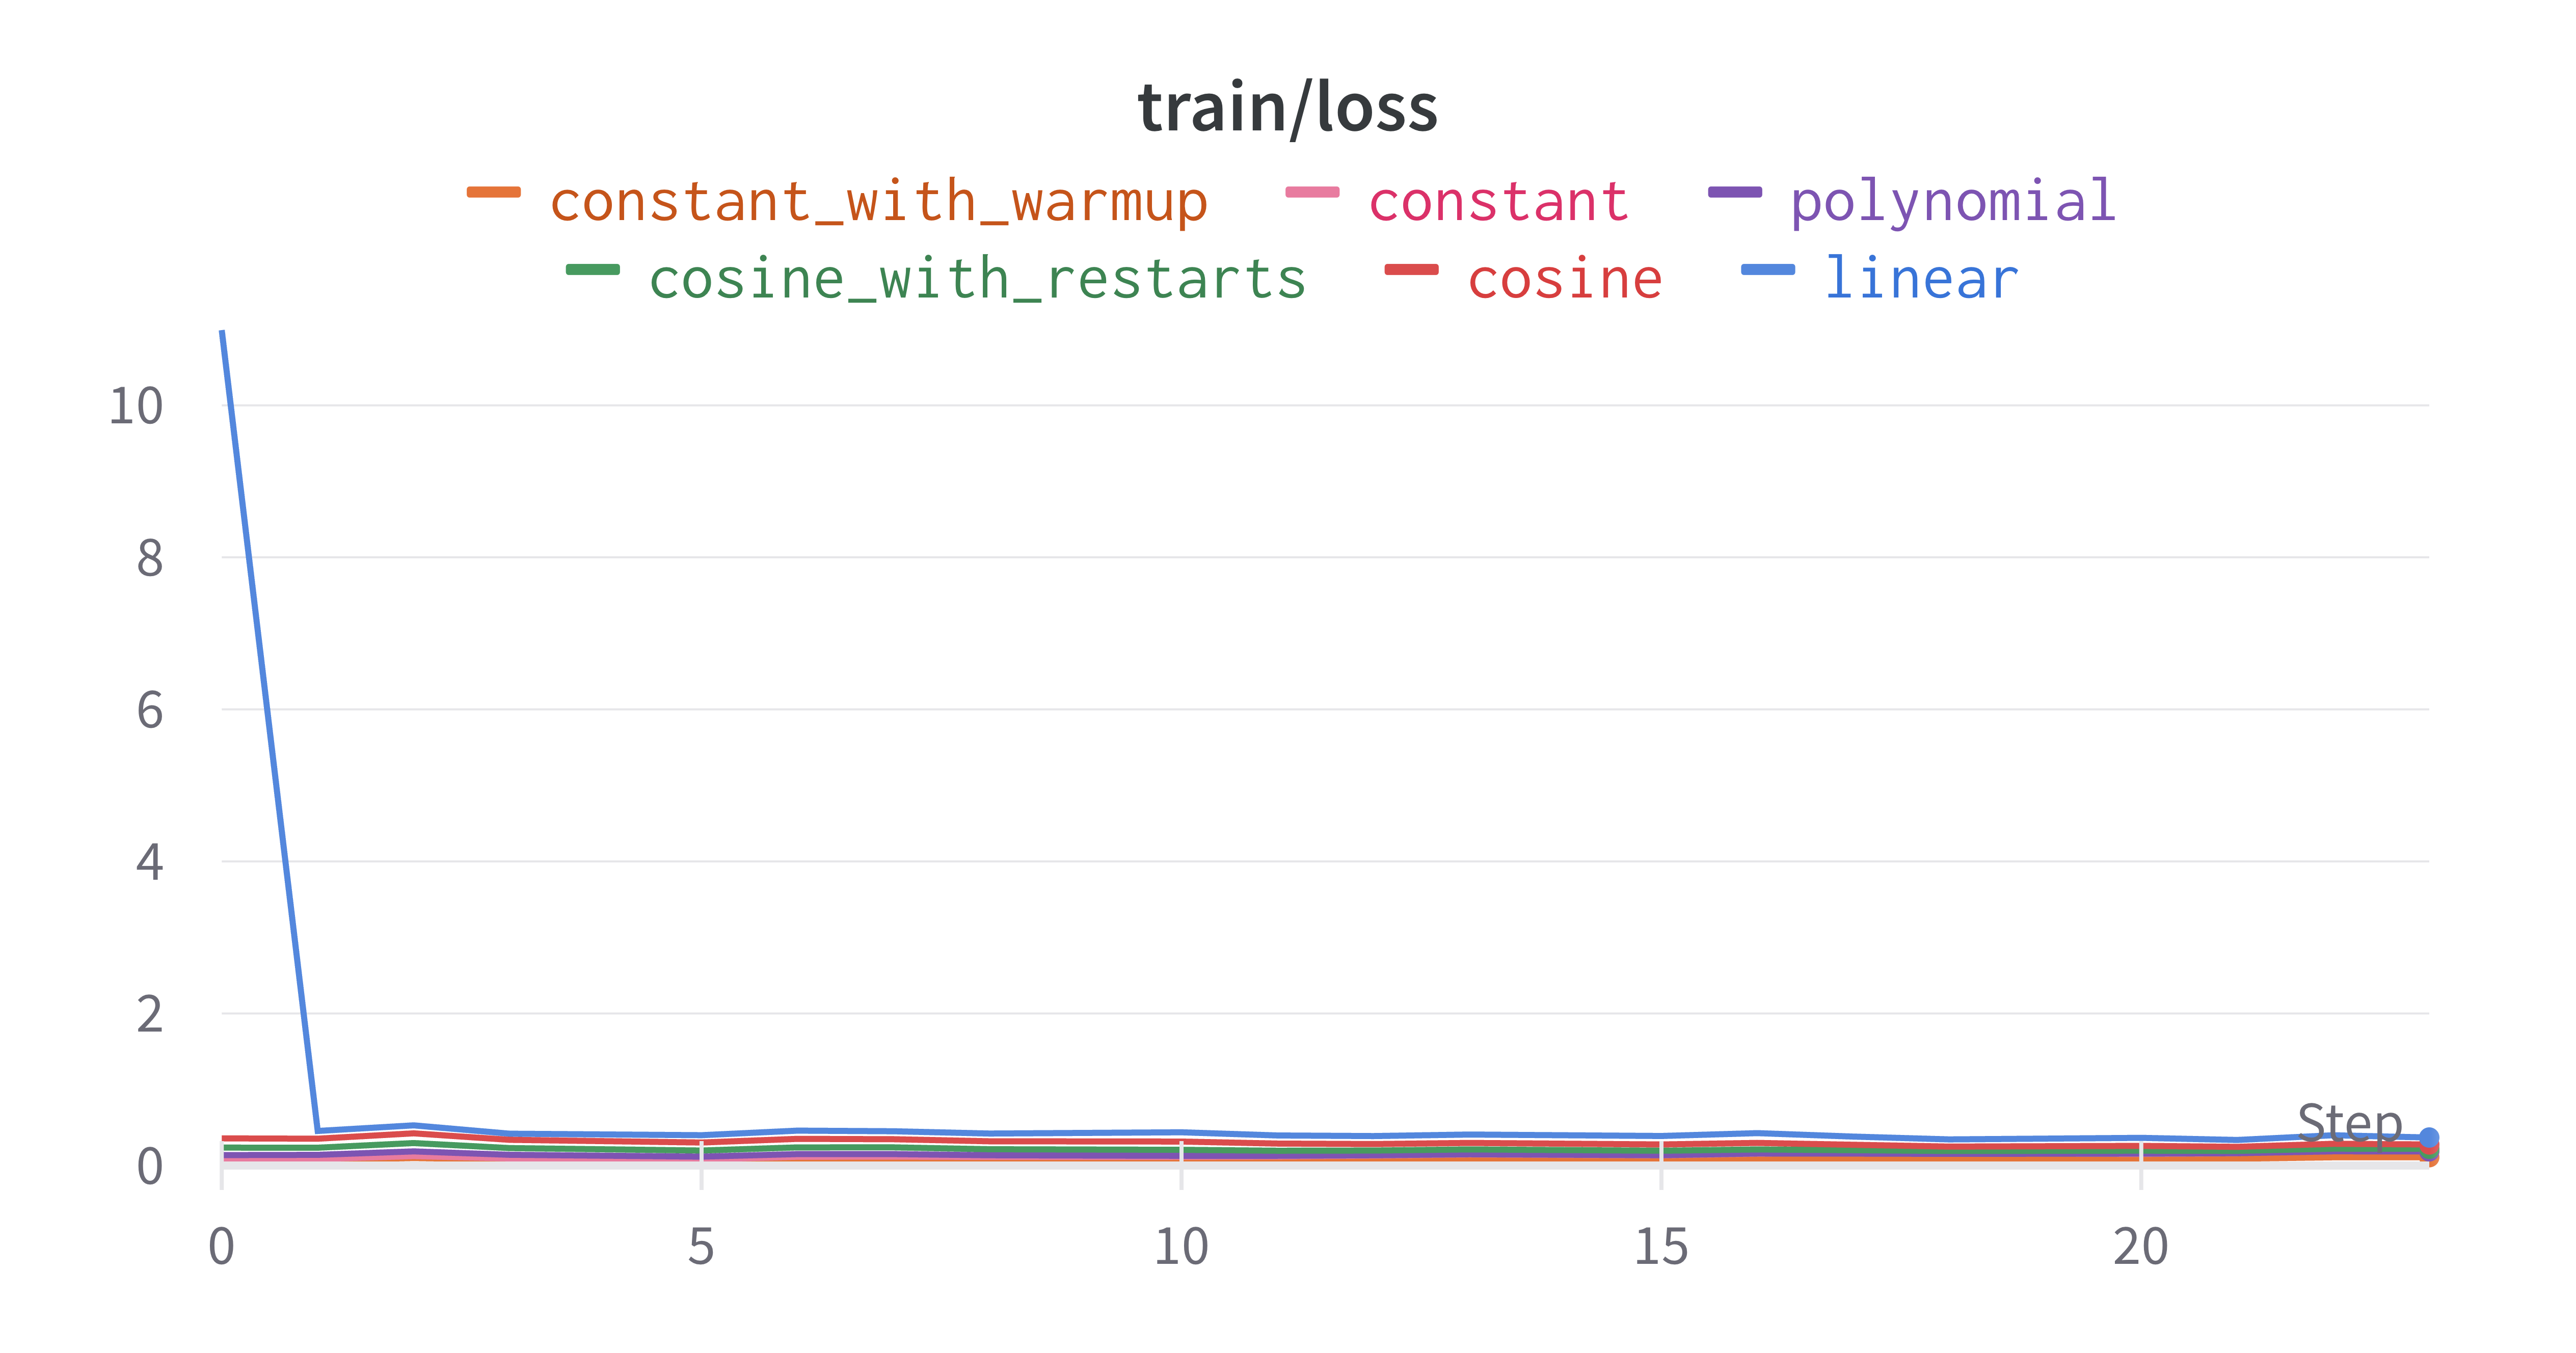
\includegraphics[width=.6\textwidth]{lr-s-train-loss}
  \caption{Значение функции ошибки на тренировочных данных}
  \label{lr-s-train-loss}
\end{figure}

\begin{figure}[H]
  \centering
  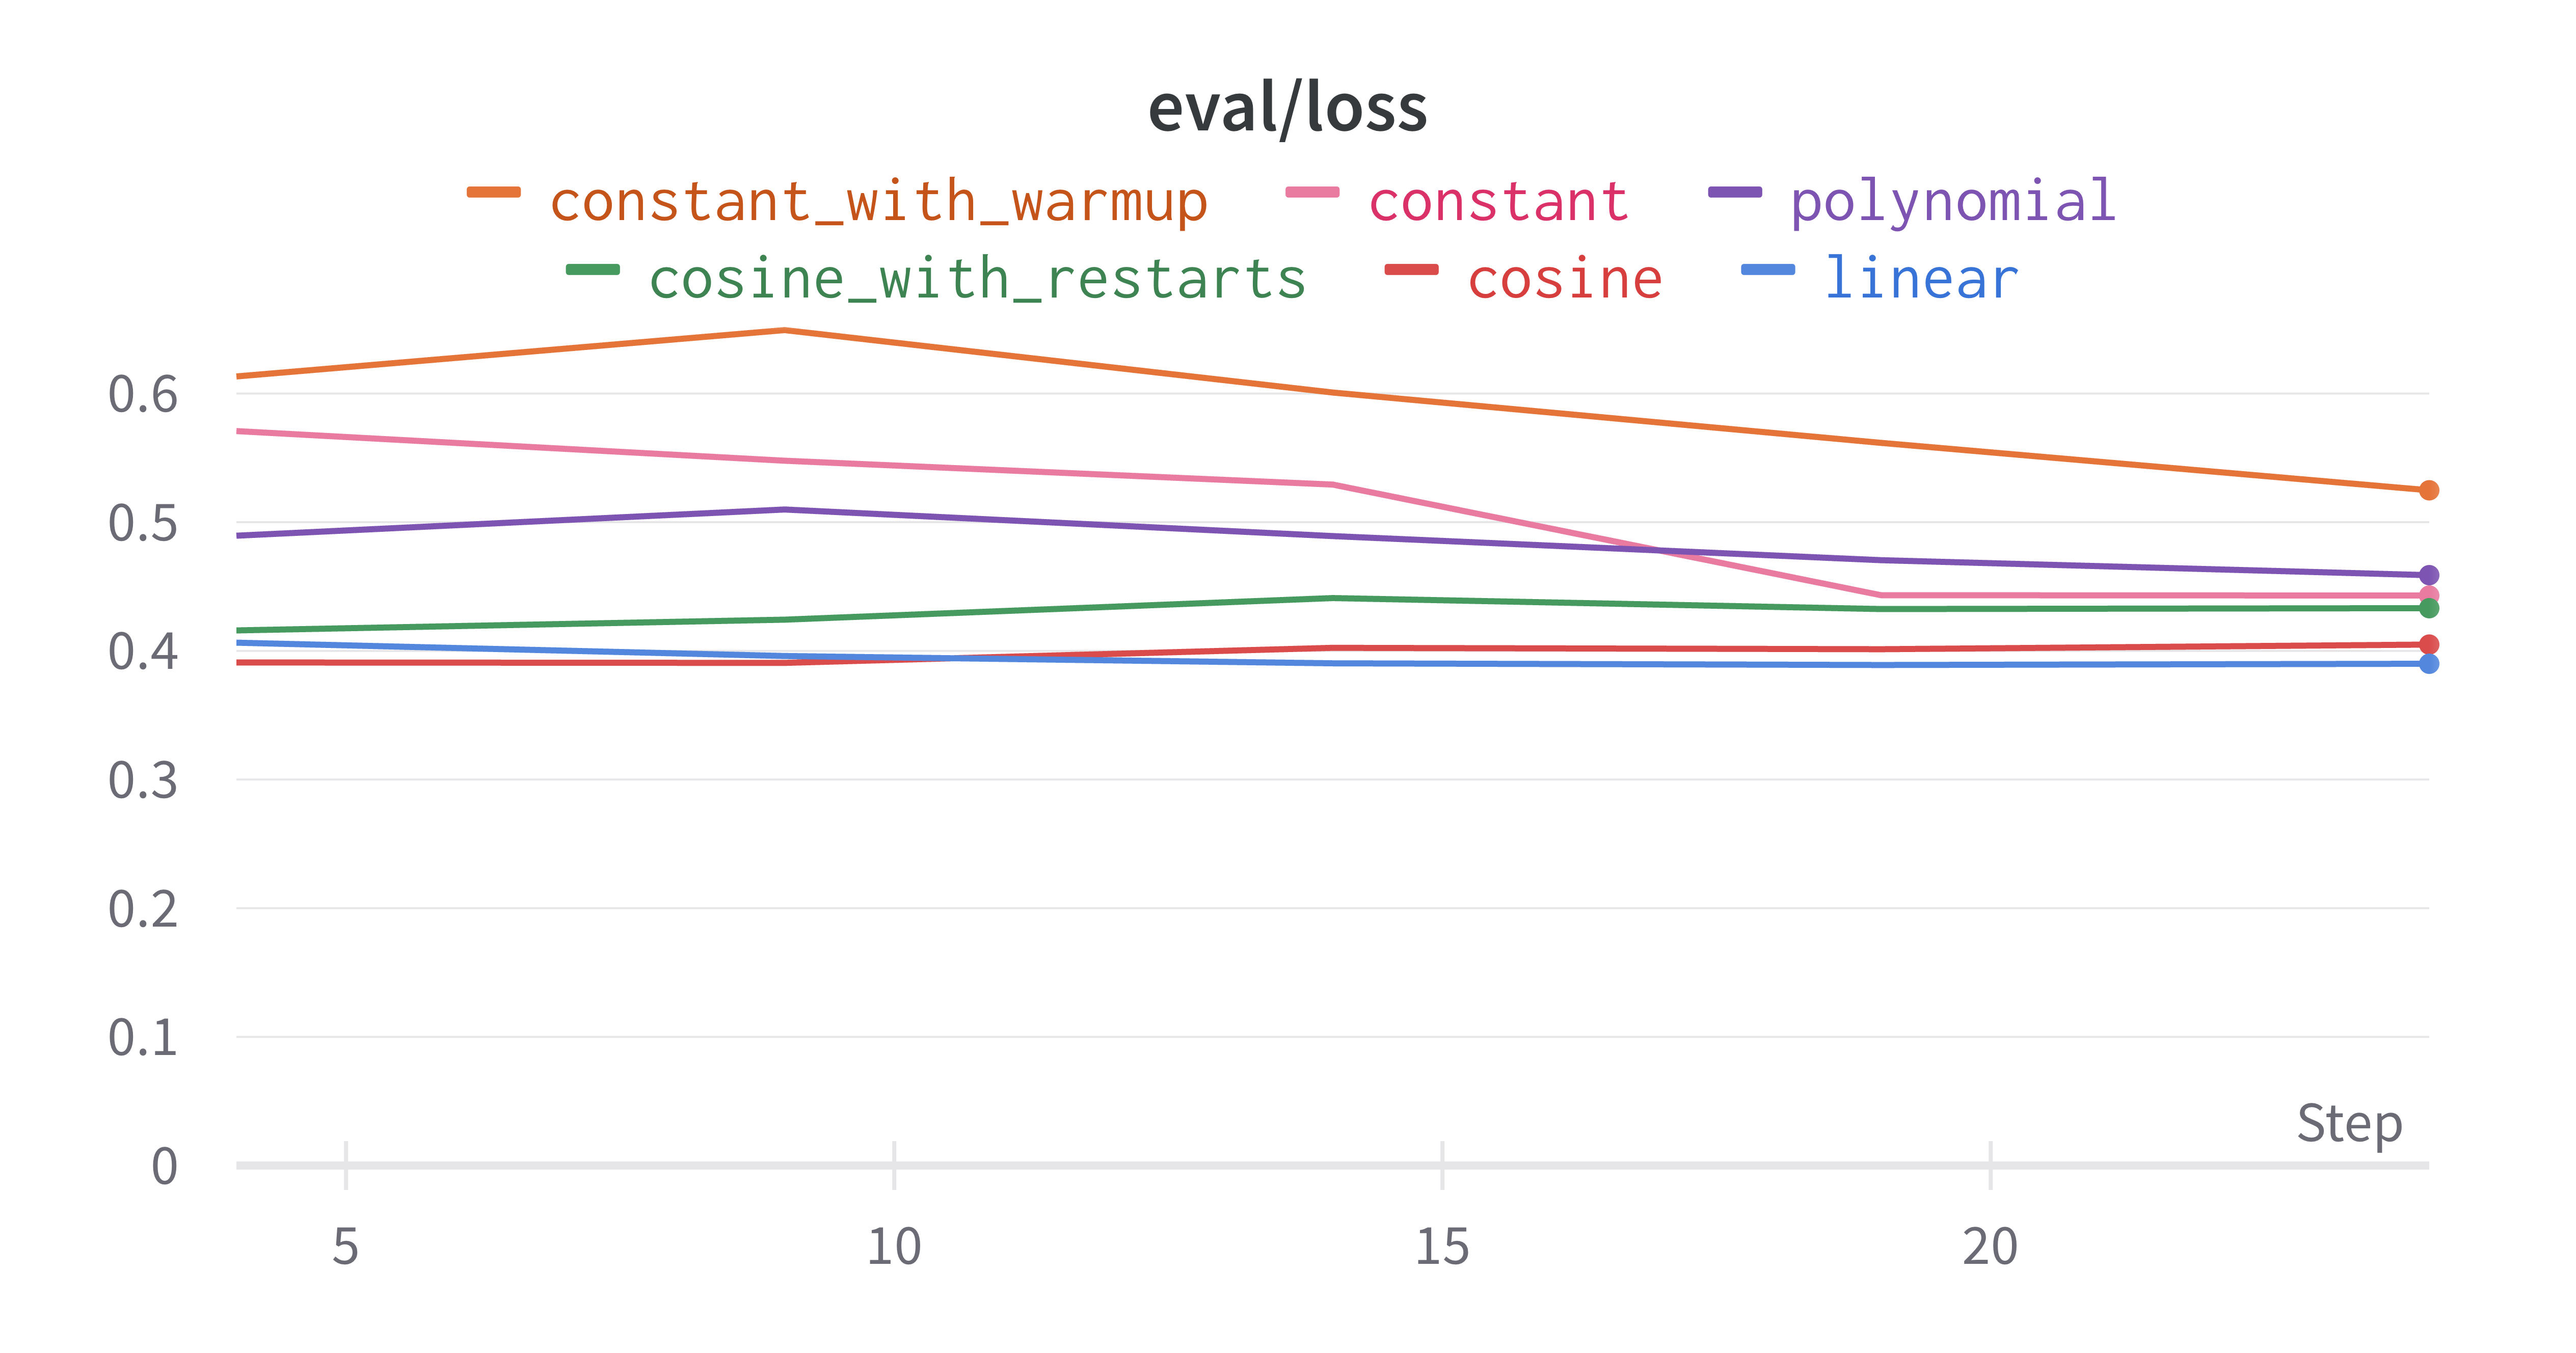
\includegraphics[width=.6\textwidth]{lr-s-eval-loss}
  \caption{Значение функции ошибки на валидационных данных}
  \label{lr-s-eval-loss}
\end{figure}

\begin{figure}[H]
  \centering
  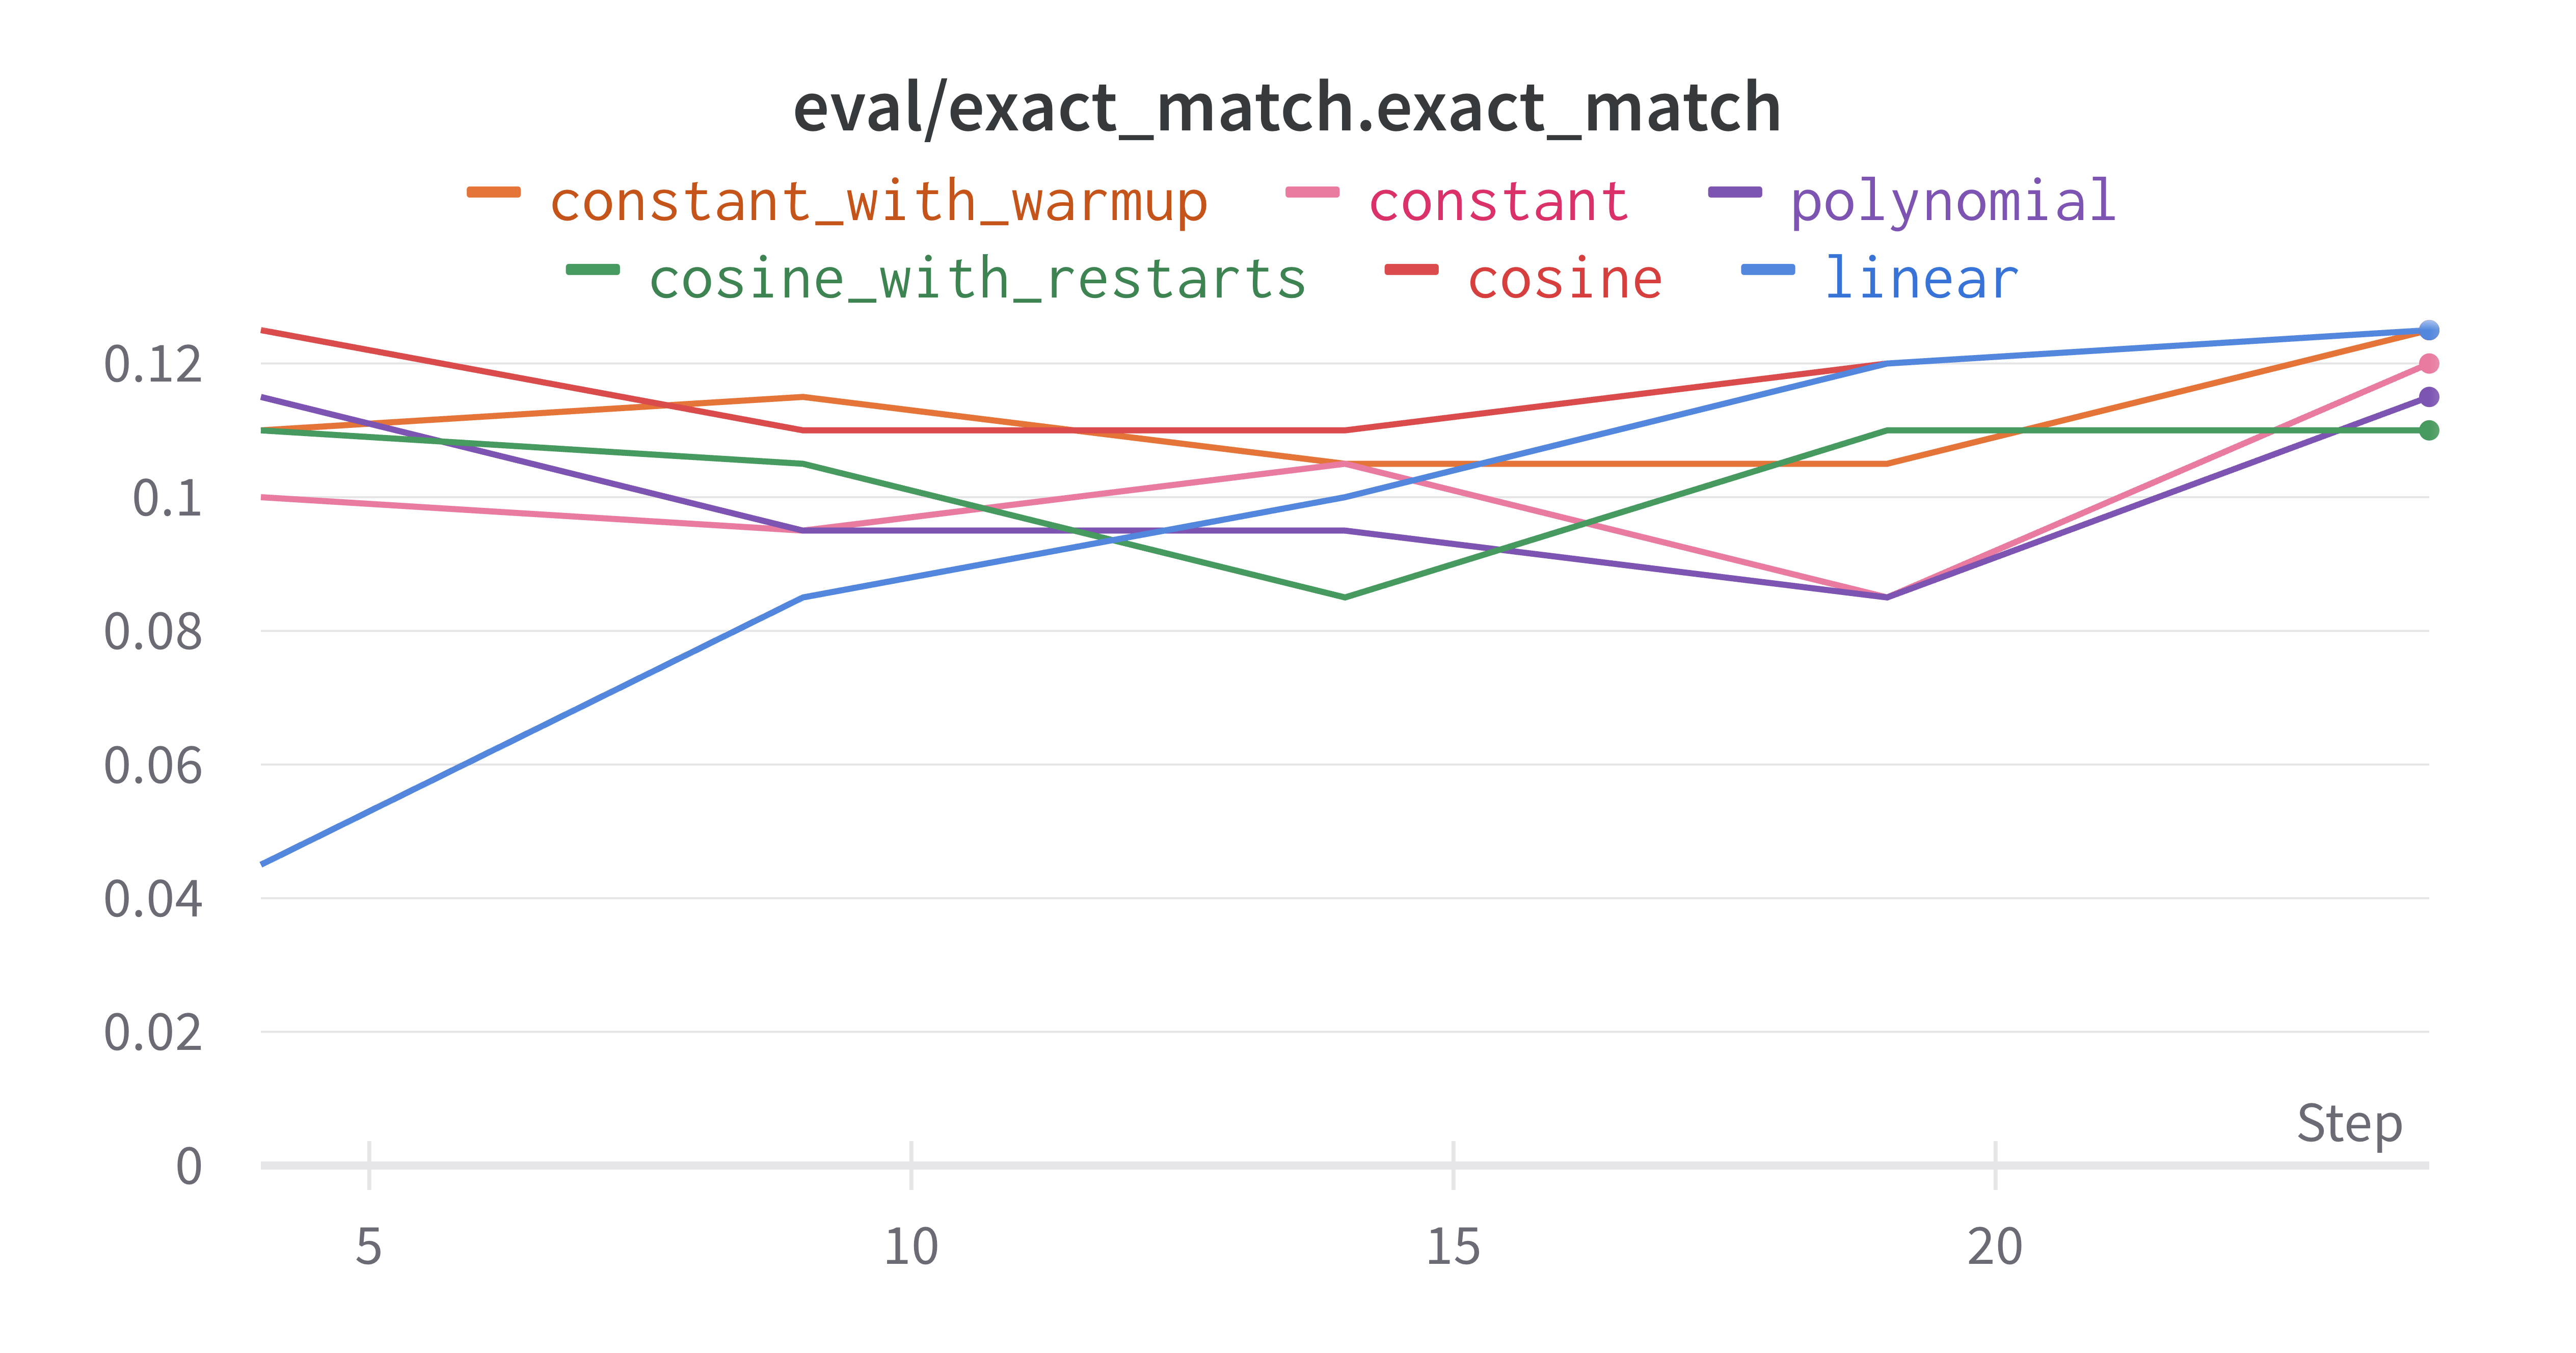
\includegraphics[width=.6\textwidth]{lr-s-em}
  \caption{Значение метрики Exact Match на валидационных данных}
  \label{lr-s-em}
\end{figure}

\begin{figure}[H]
  \centering
  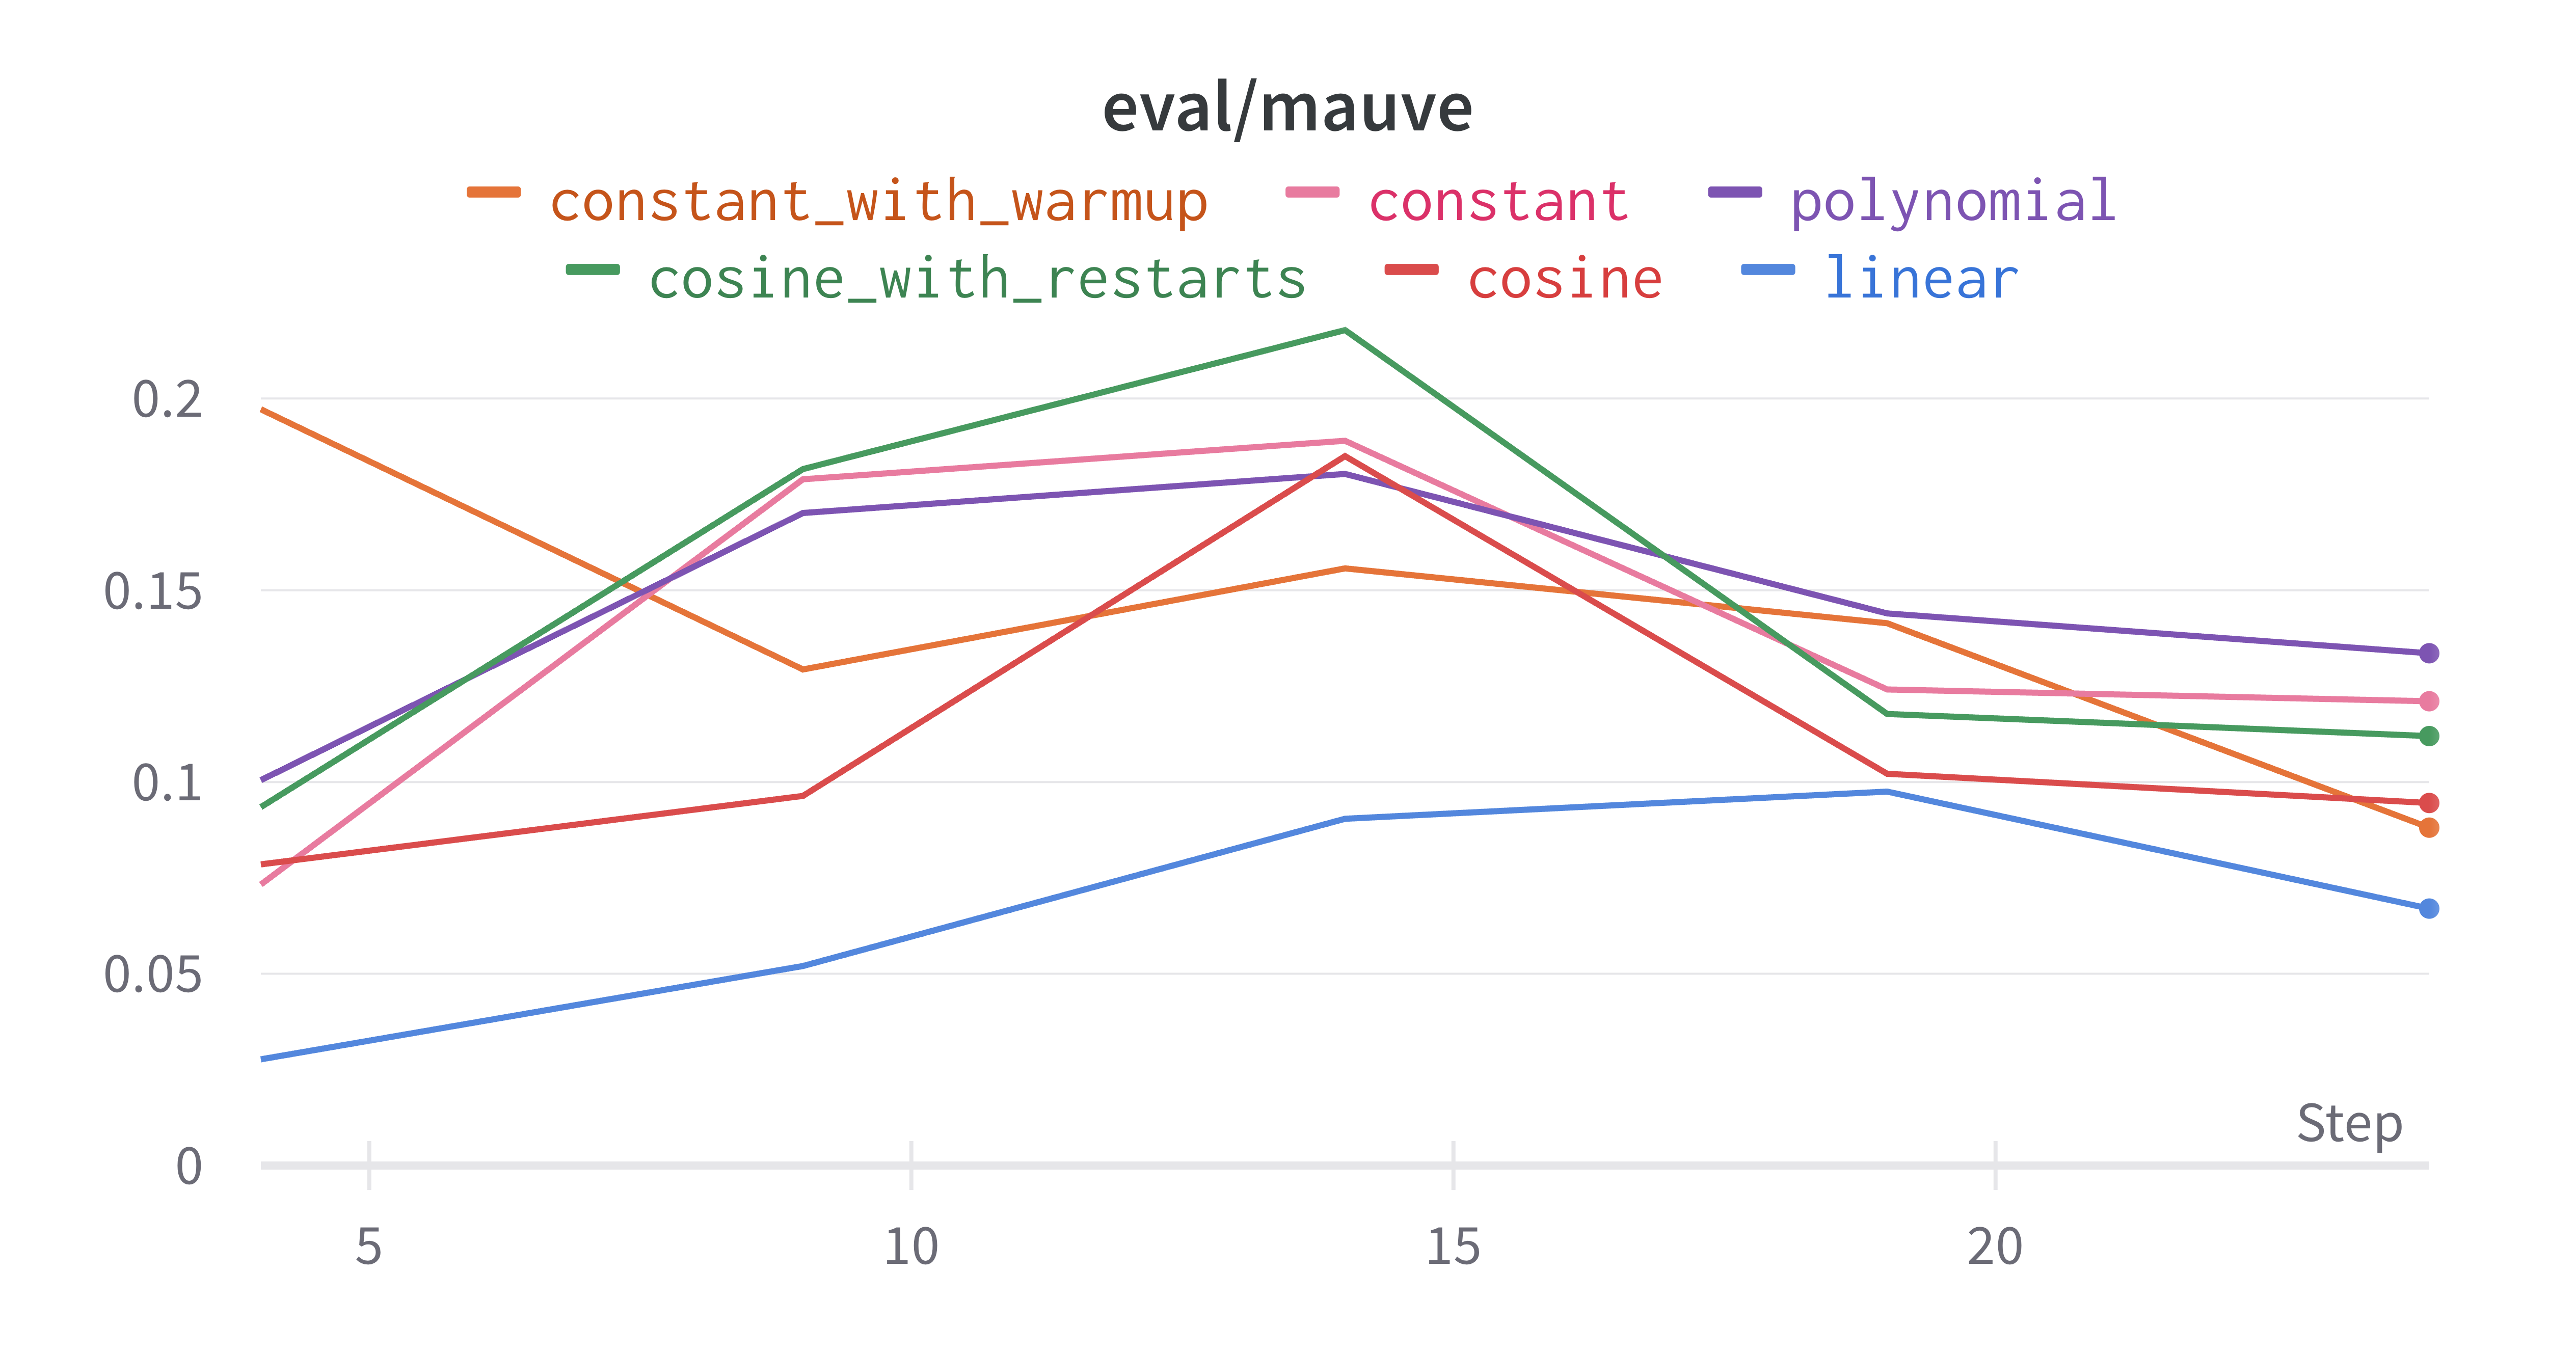
\includegraphics[width=.6\textwidth]{lr-s-mauve}
  \caption{Значение метрики MAUVE на валидационных данных}
  \label{lr-s-mauve}
\end{figure}

\begin{figure}[H]
  \centering
  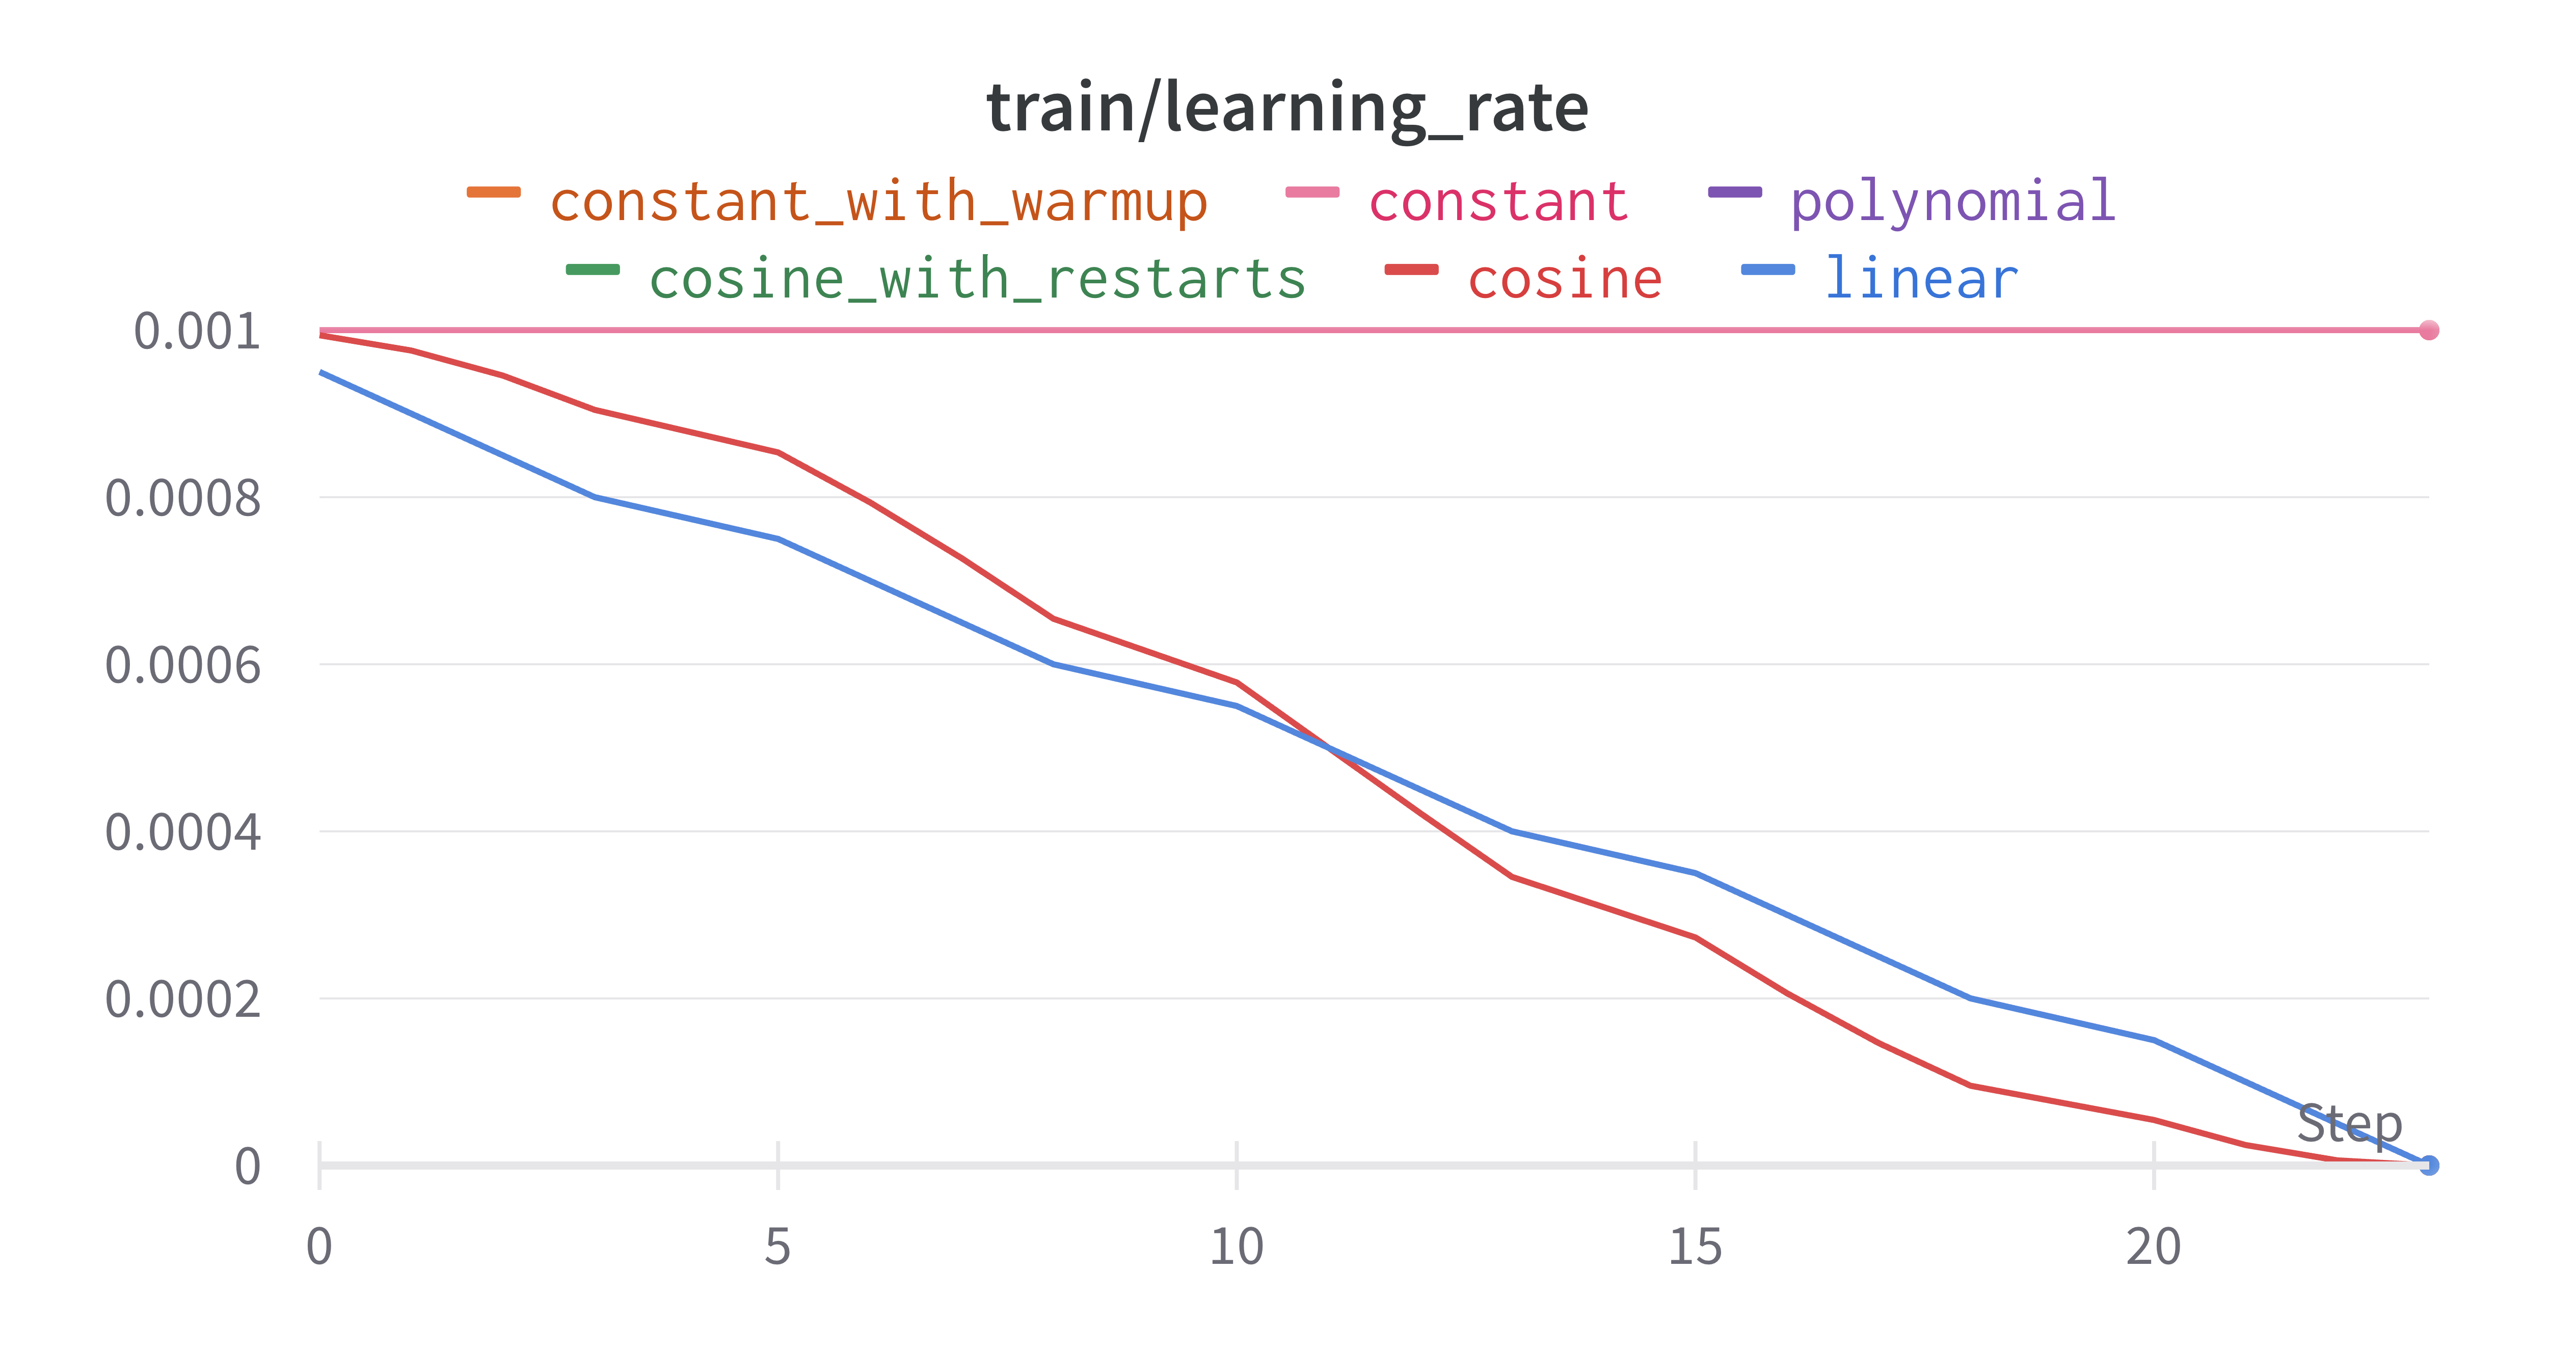
\includegraphics[width=.6\textwidth]{lr-s-lr}
  \caption{График изменения скорости обучения}
  \label{lr-s-lr}
\end{figure}

В следующих экспериментах при зафиксированном константном планировщике скорости обучения искалась наиболее эффективная скорость обучения. Стоит отметить, что при скорости обучения равной $1 \times 10^{-4}$ процесс обучения не завершился успешно. Из рисунков \ref{lr-train-loss}, \ref{lr-eval-loss}, \ref{lr-em}, \ref{lr-mauve} видно, что значения, близкие к $4 \times 10^{-4}$ и к $9 \times 10^{-4}$ показывают лучшие значения функций ошибок на всех выборках и лучшие значения метрик. Значение скорости обучения $9 \times 10^{-4}$ показывает результаты чуть лучше, чем $4 \times 10^{-4}$, быстрее достигая лучших значений. В целом, почти все значения скорости обучения показывают схожие результаты, но выбор оптимальных параметров для обучения на большей выборке может сказаться на качестве модели.

% LR
\begin{figure}[H]
  \centering
  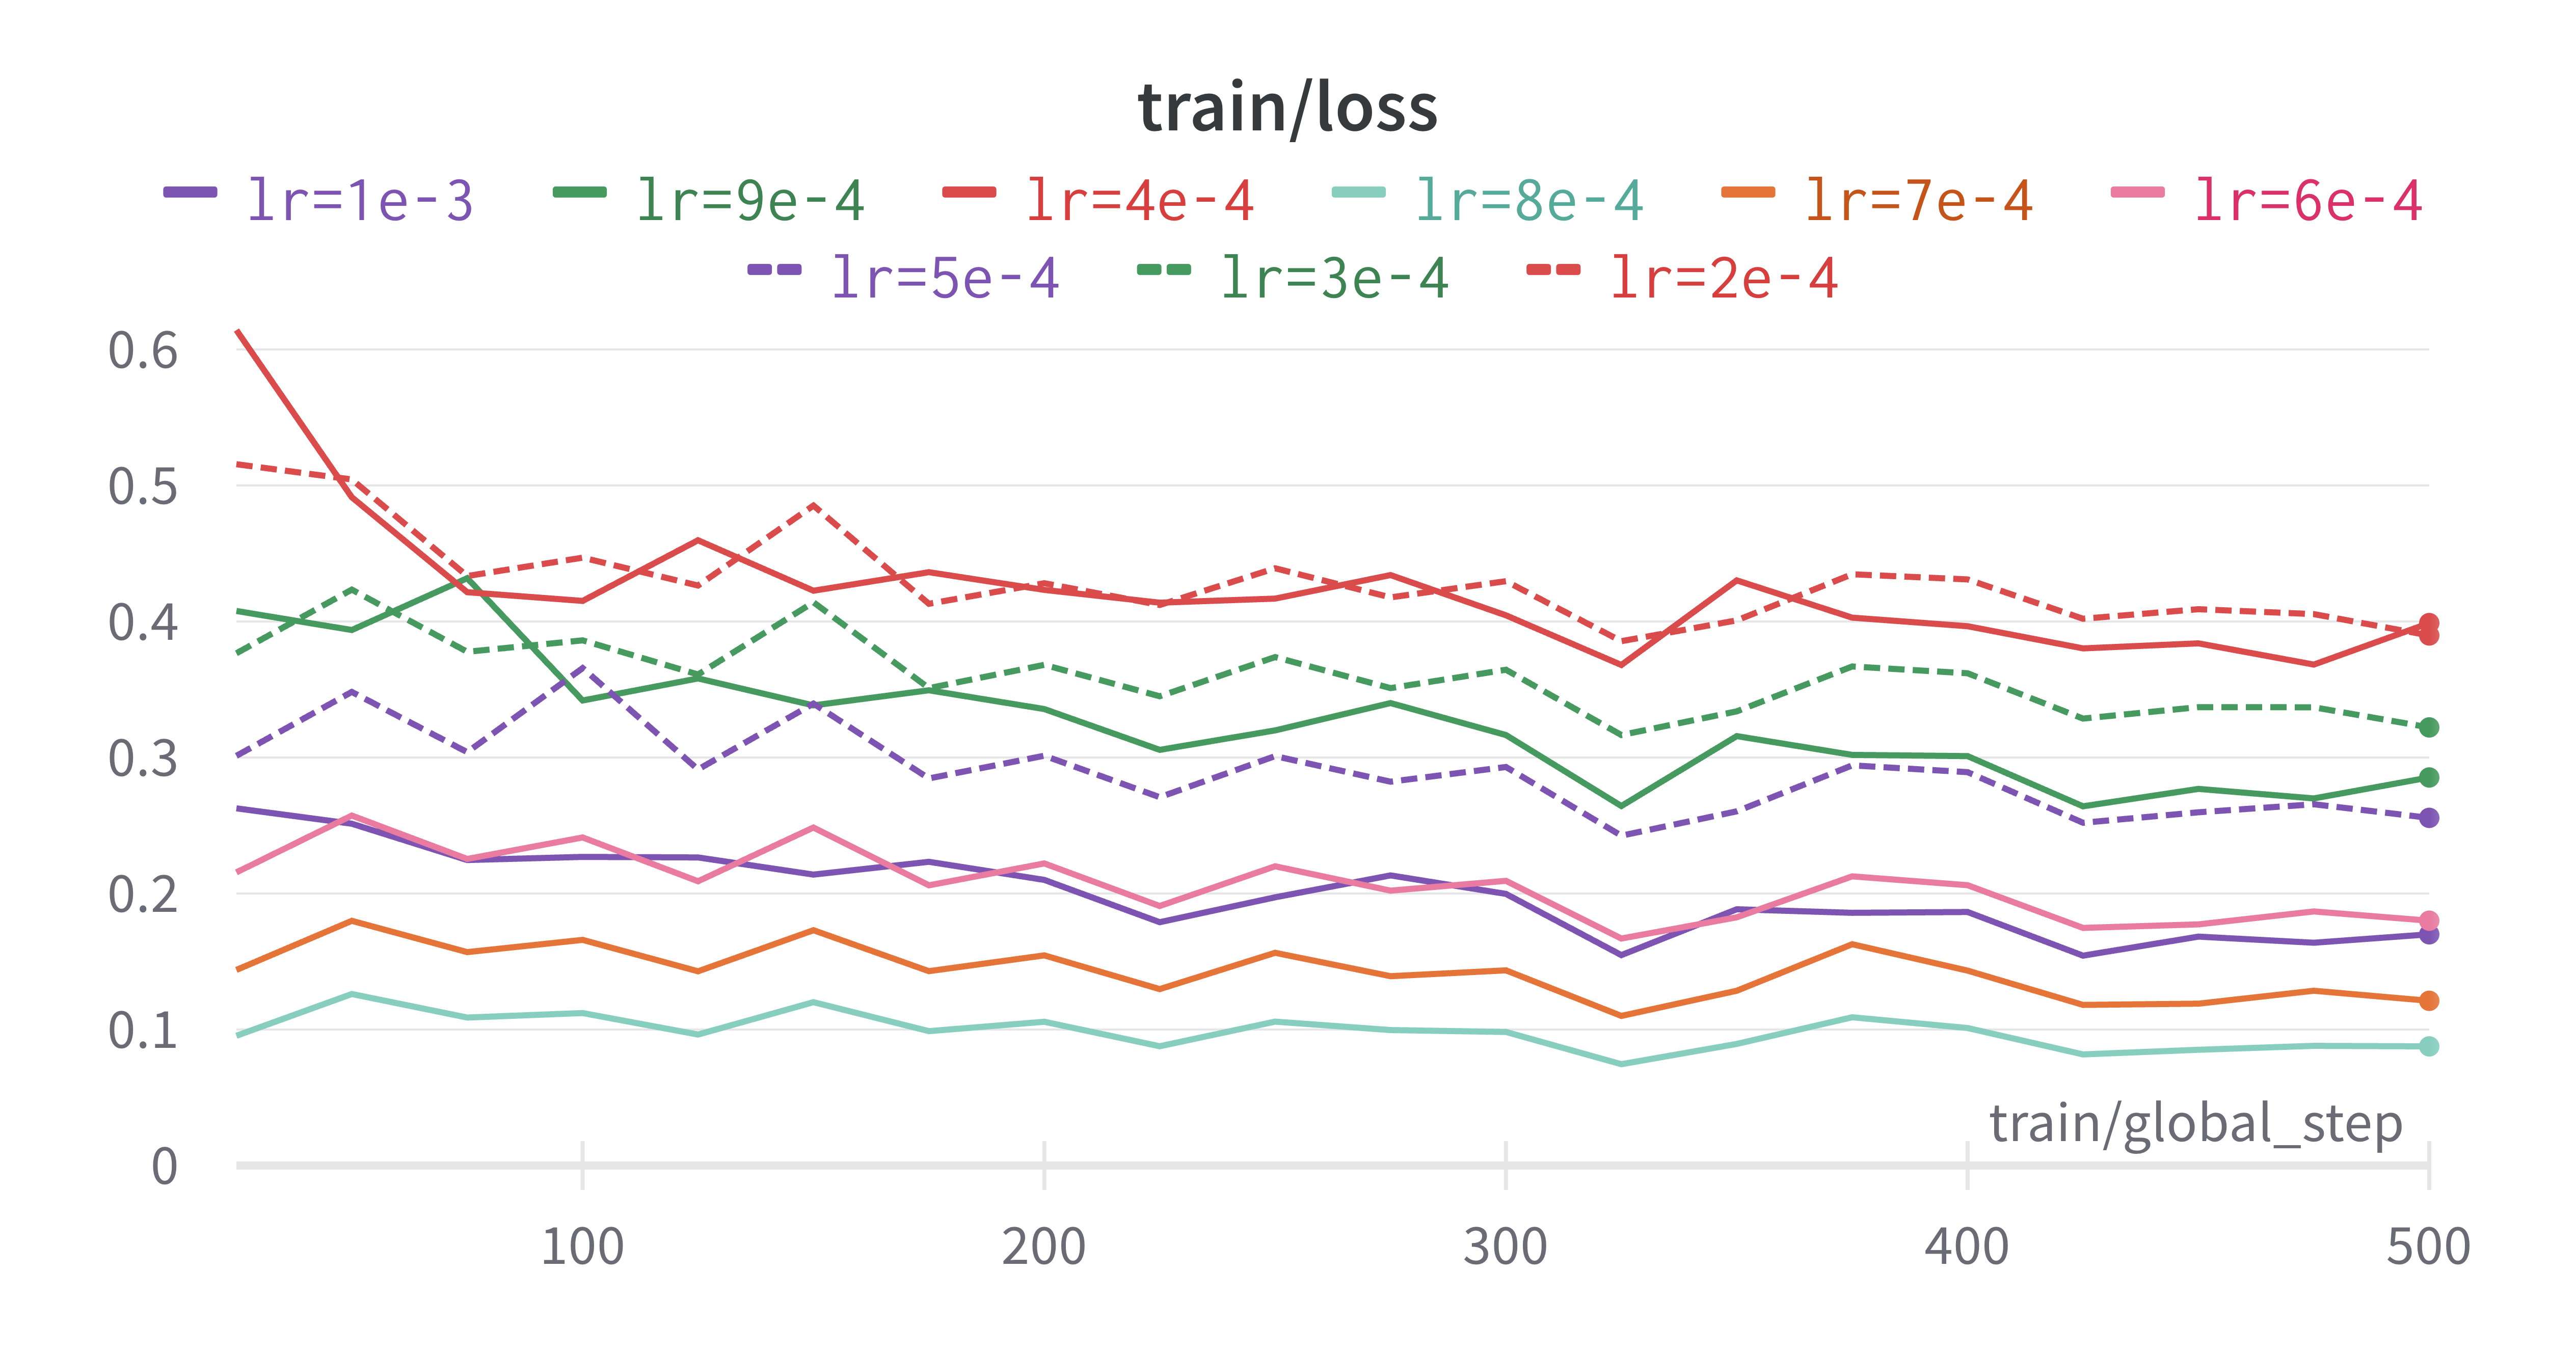
\includegraphics[width=.6\textwidth]{lr-train-loss}
  \caption{Значение функции ошибки на тренировочных данных}
  \label{lr-train-loss}
\end{figure}

\begin{figure}[H]
  \centering
  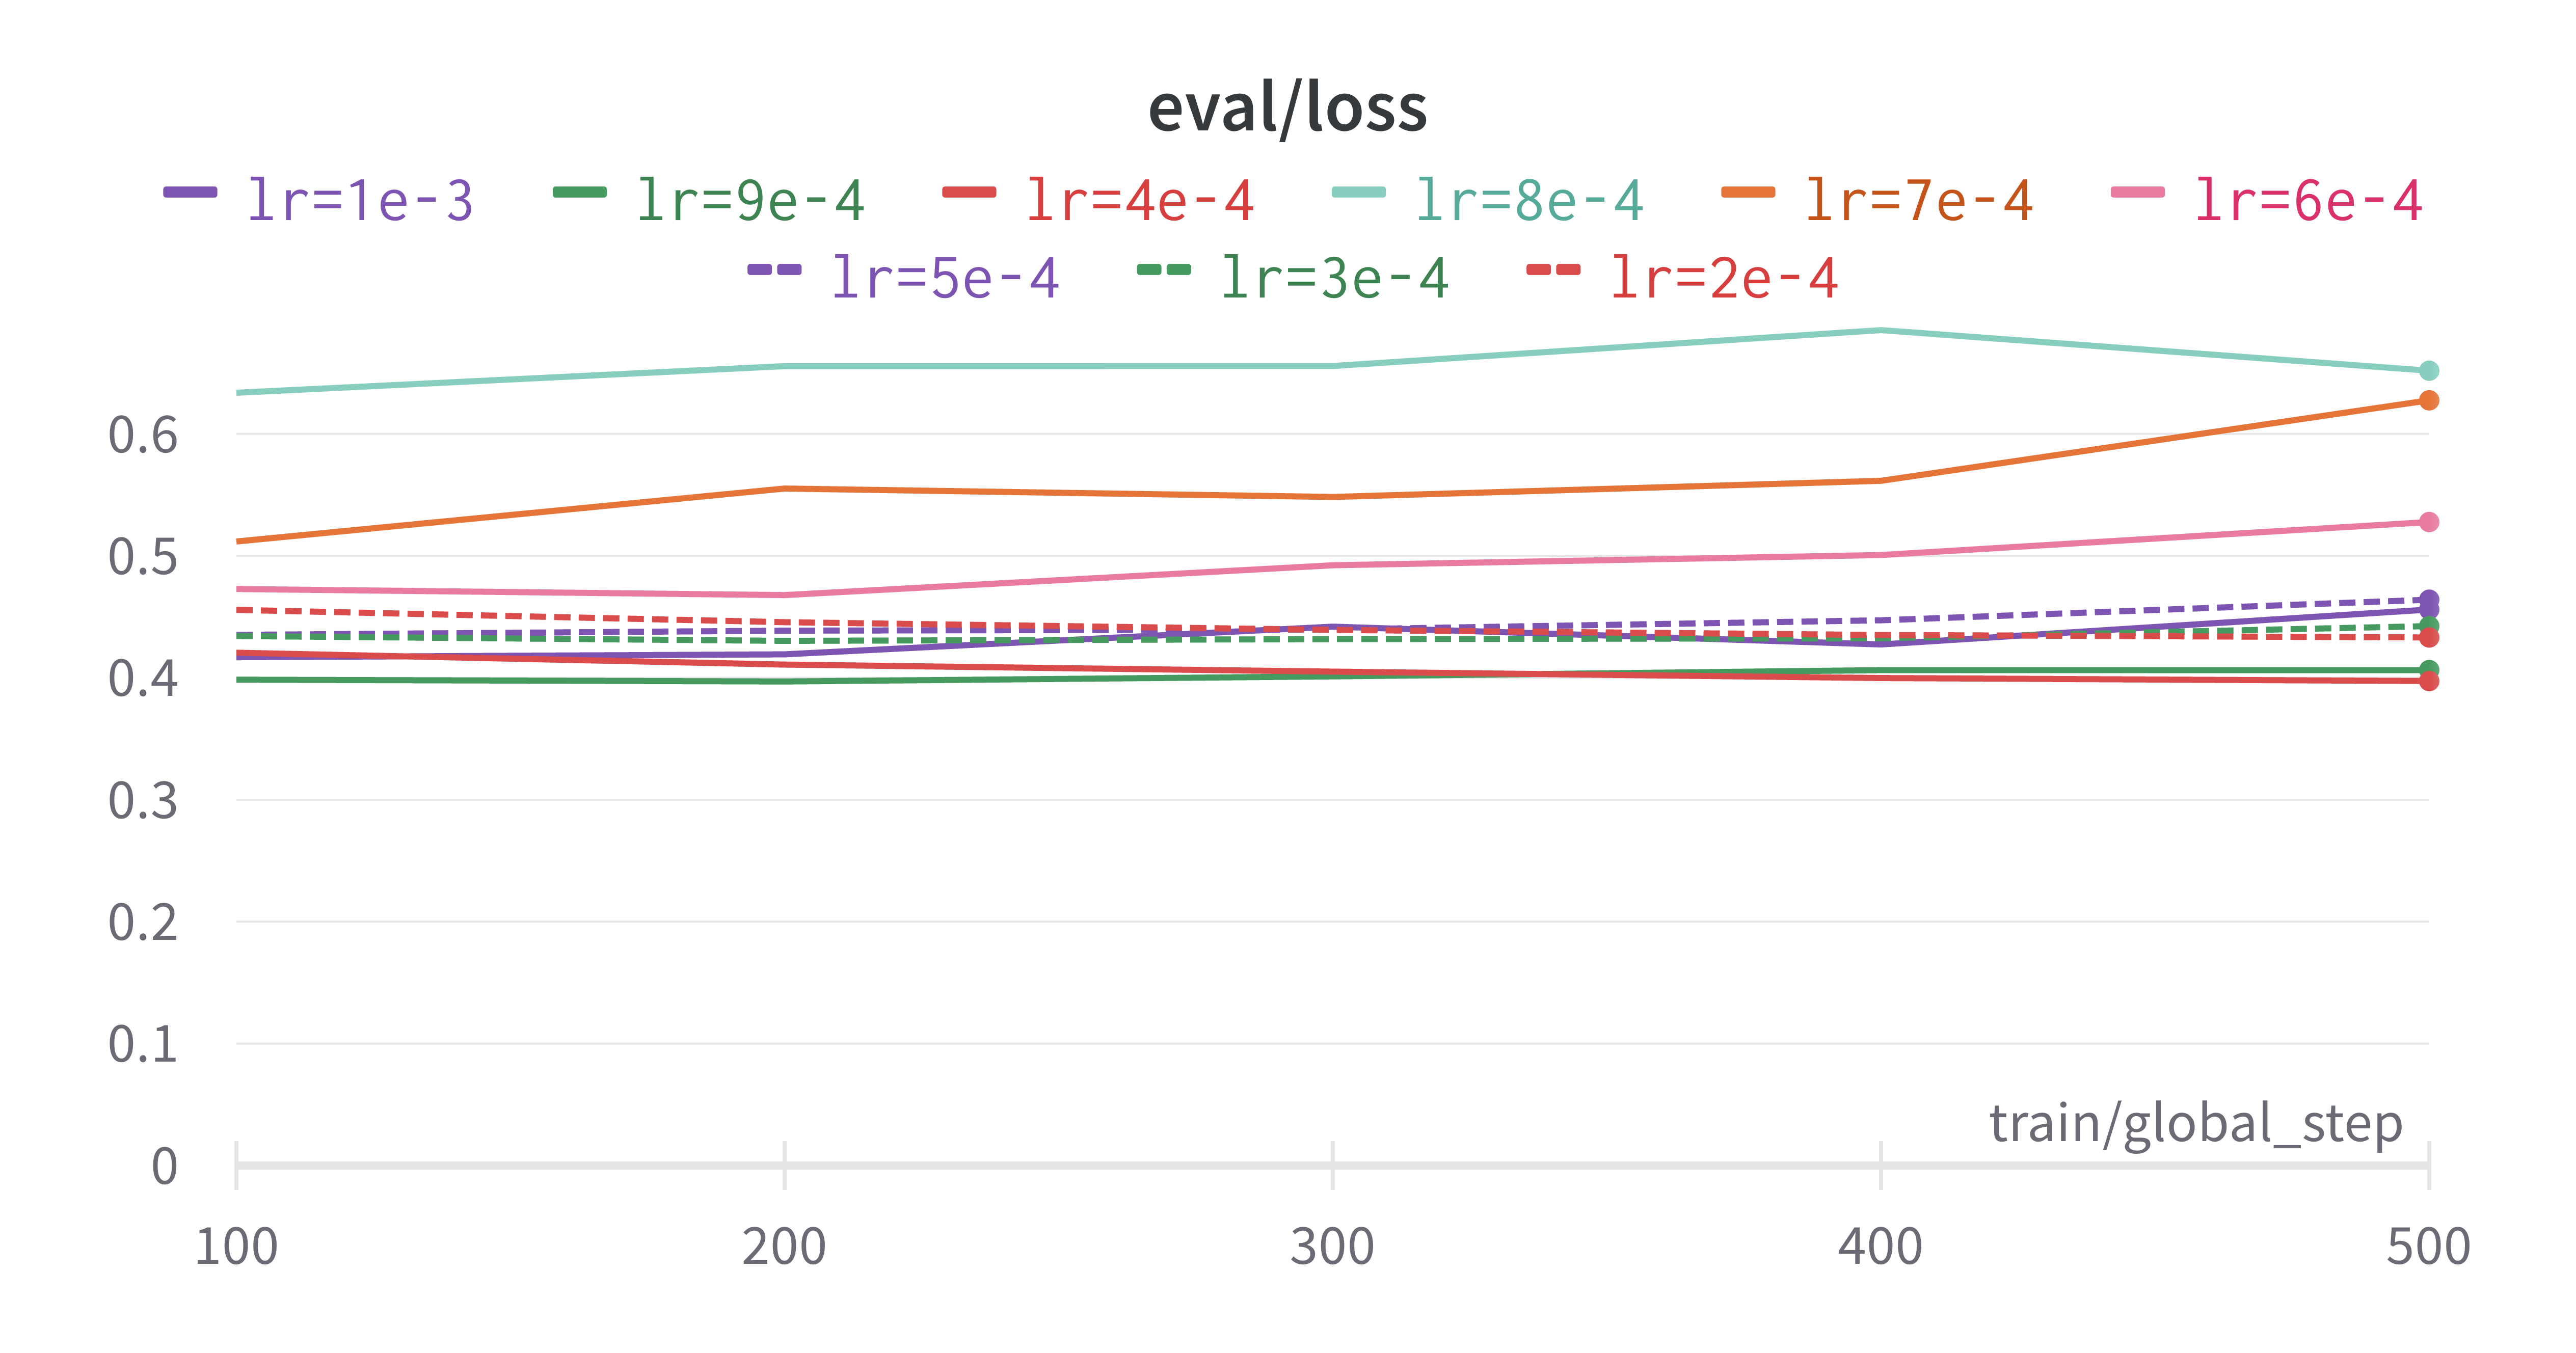
\includegraphics[width=.6\textwidth]{lr-eval-loss}
  \caption{Значение функции ошибки на валидационных данных}
  \label{lr-eval-loss}
\end{figure}

\begin{figure}[H]
  \centering
  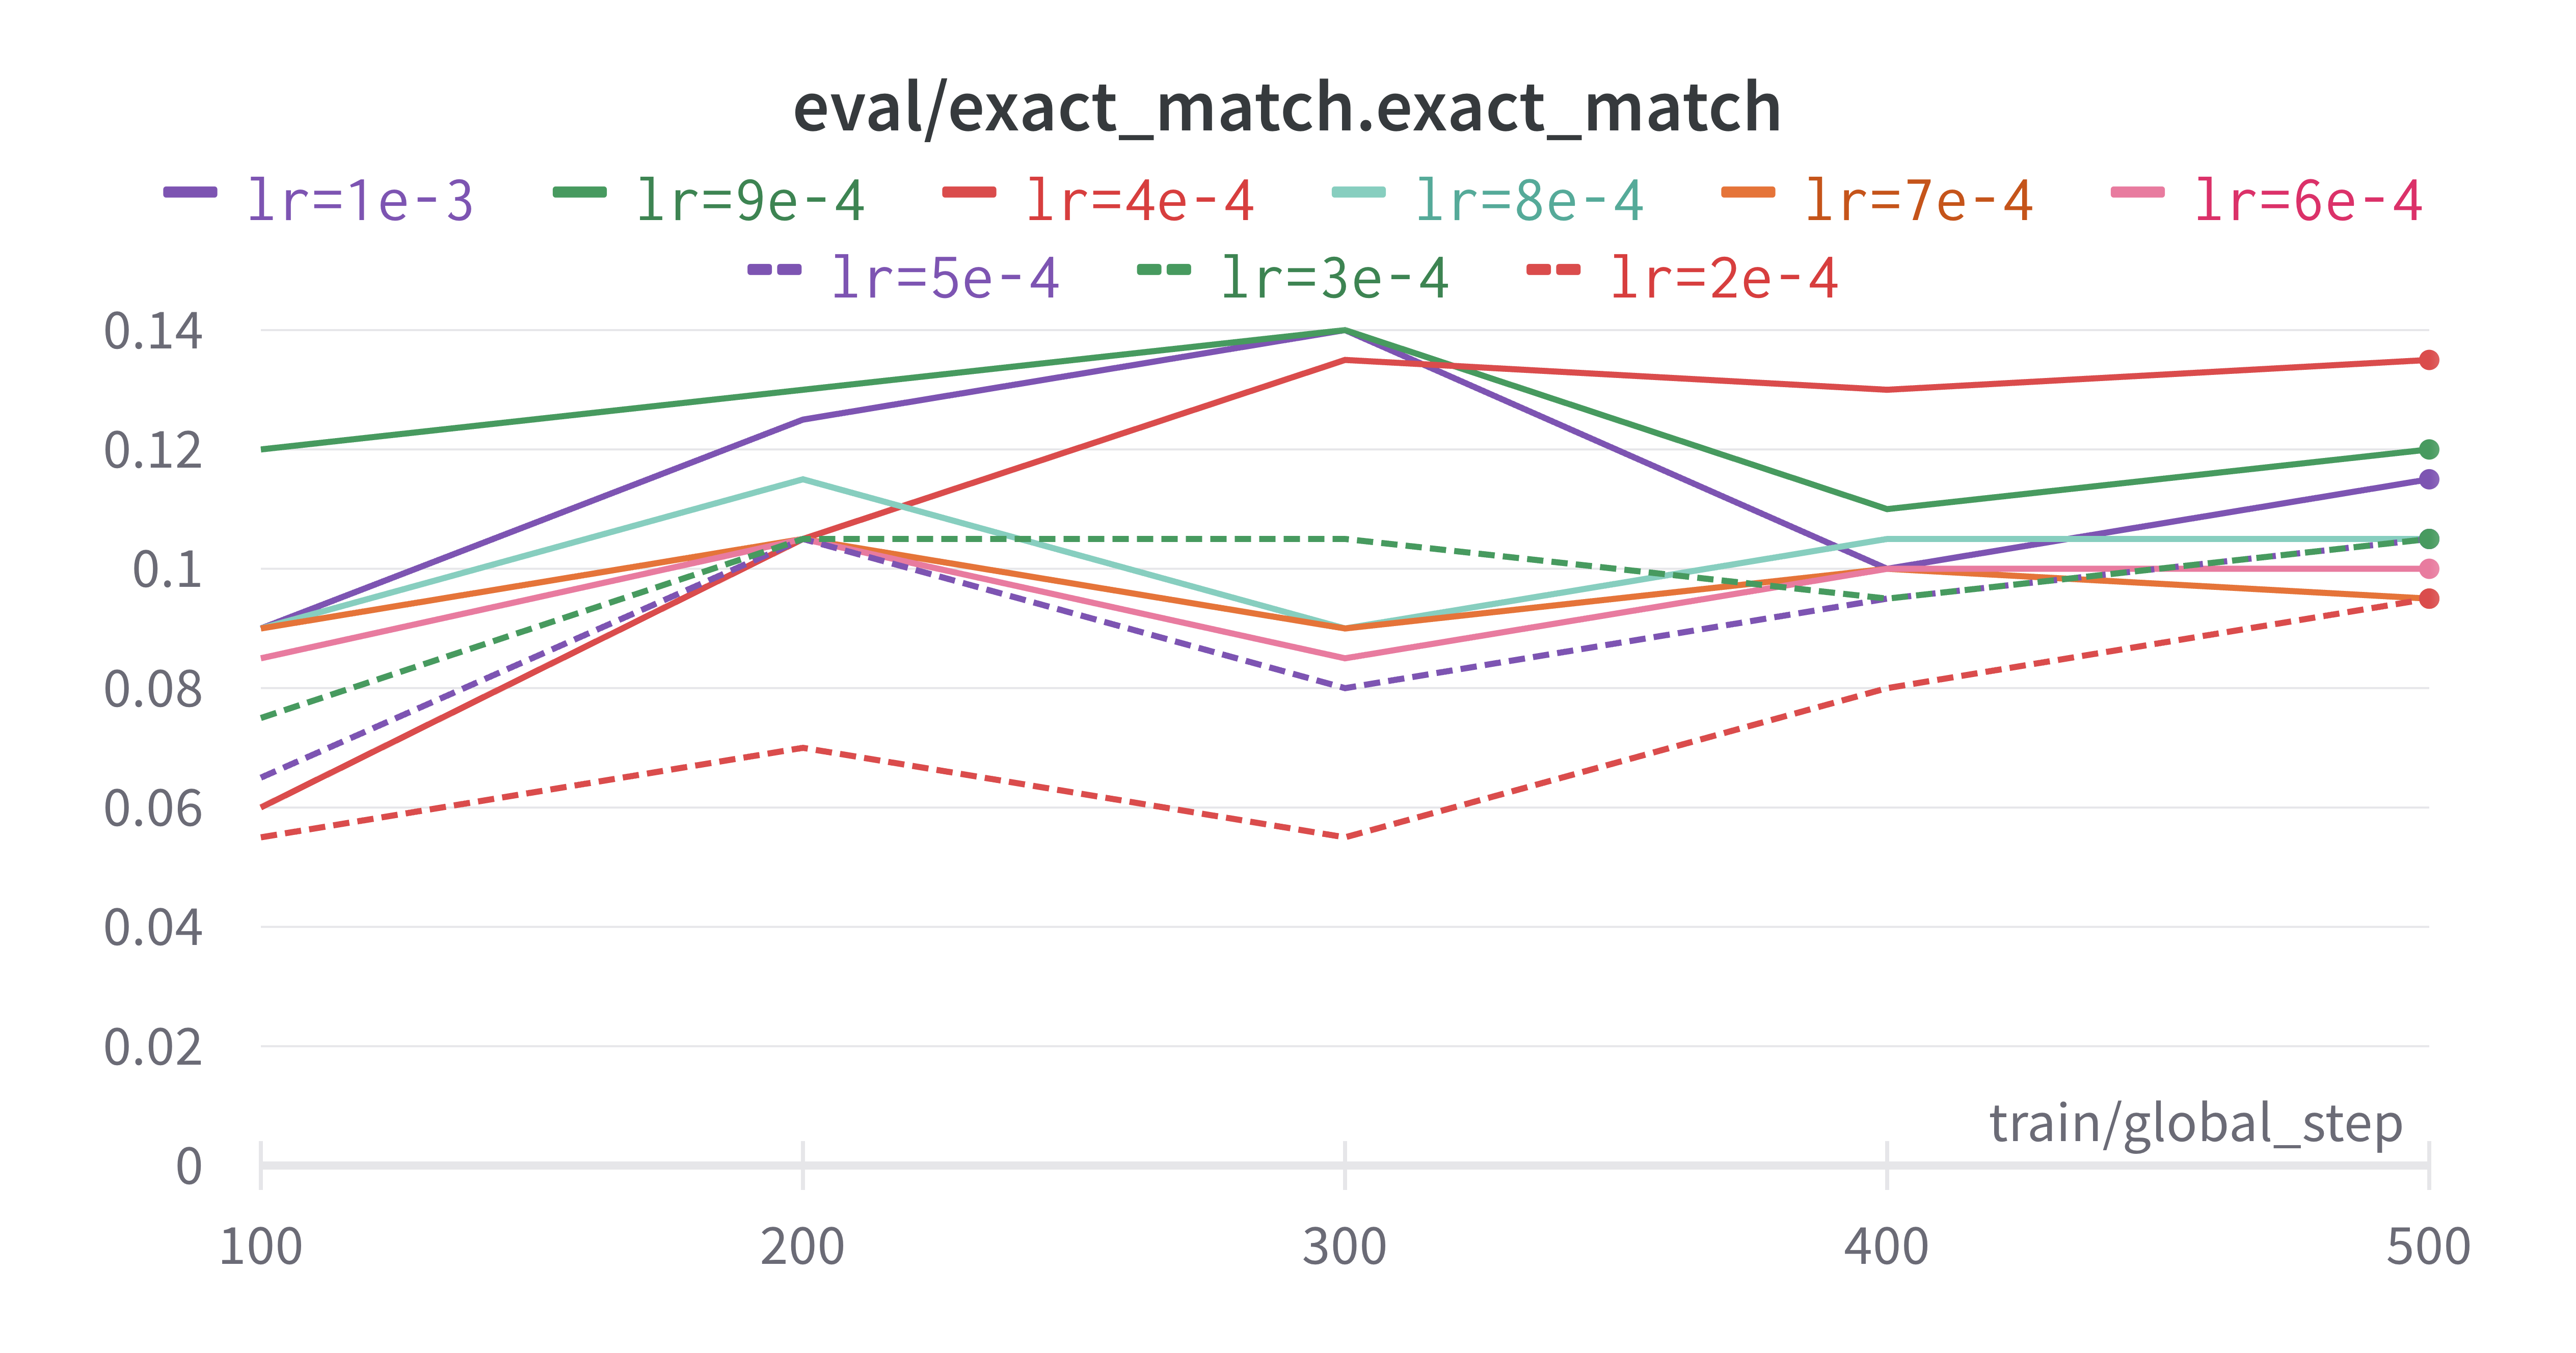
\includegraphics[width=.6\textwidth]{lr-em}
  \caption{Значение метрики Exact Match на валидационных данных}
  \label{lr-em}
\end{figure}

\begin{figure}[H]
  \centering
  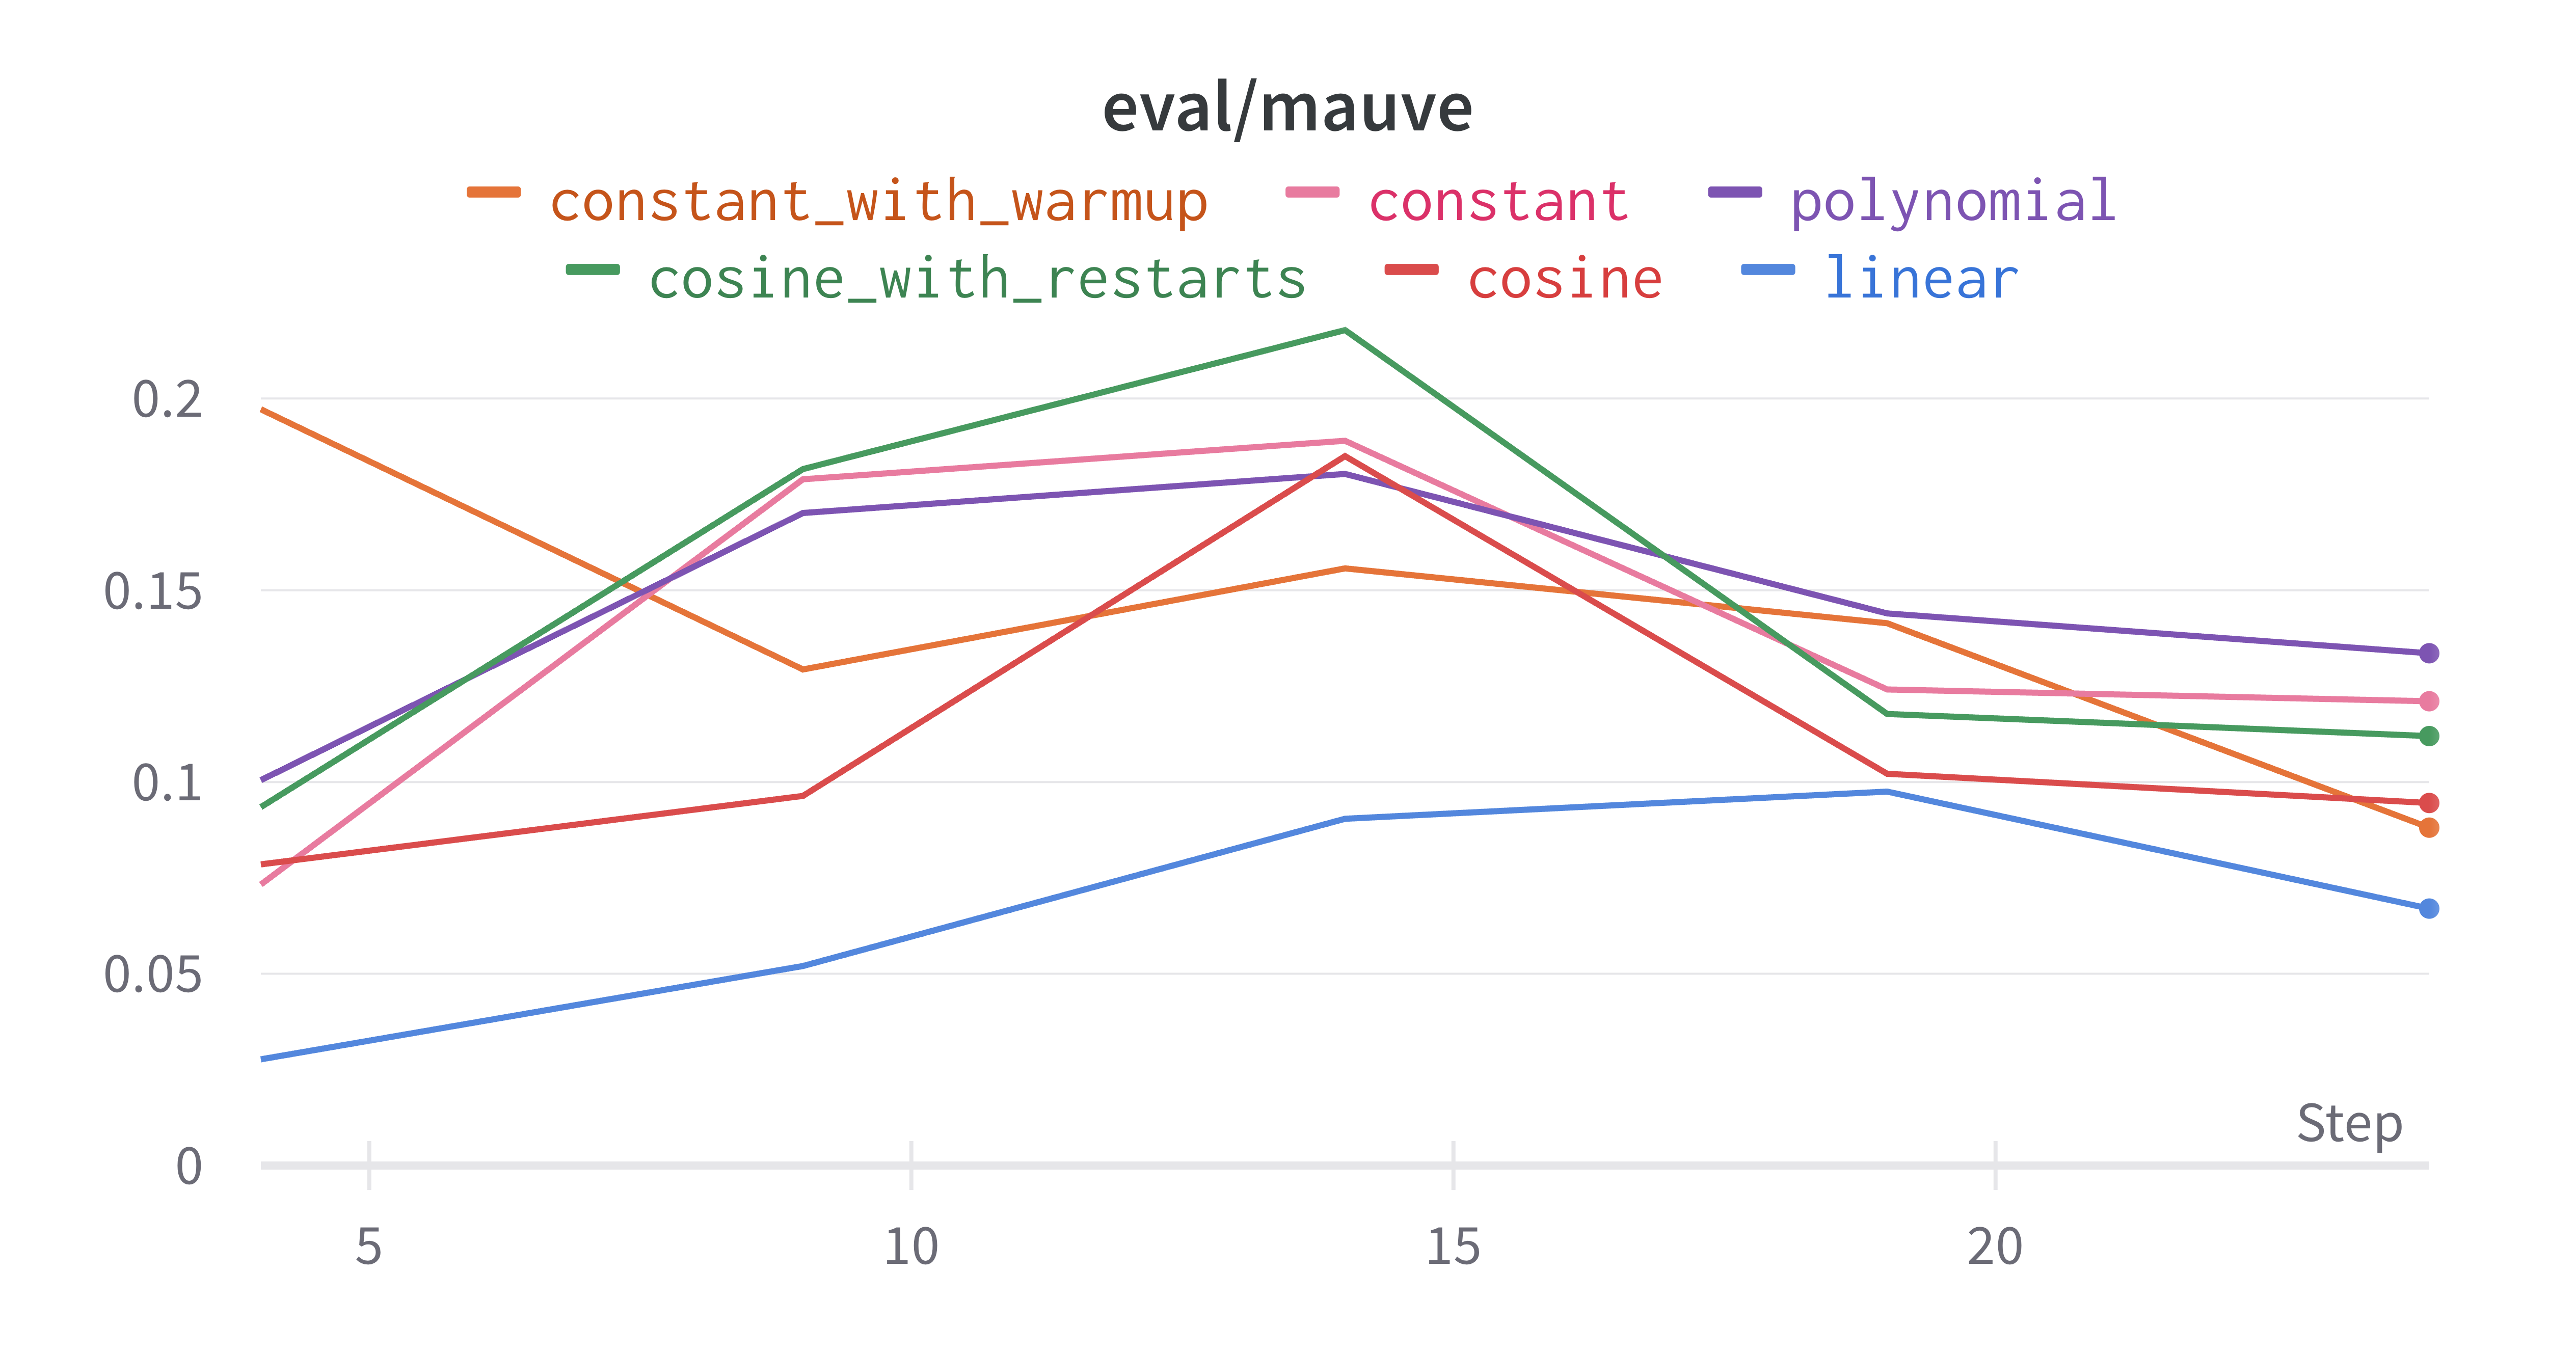
\includegraphics[width=.6\textwidth]{lr-s-mauve}
  \caption{Значение метрики MAUVE на валидационных данных}
  \label{lr-mauve}
\end{figure}

Исходя из всех экспериментов можно сделать вывод, что оптимальные параметры для обучения будут константный планировщик скорости обучения и скорость обучения со значением $9 \times 10^{-4}$

\section{ОБУЧЕНИЕ ИТОГОВОЙ МОДЕЛИ}

С подобранными ранее параметрами на была обучена итоговая модель. Общее количество операций, произведенных во время обучения, составило $2 \times 10^{18}$. Количество токенов, которые фигурировали в процессе обучения -- $25 \times 10^{6}$. Процесс обучения виден на рисунках \ref{total-train-loss}, \ref{total-eval-loss}, \ref{total-em}, \ref{total-mauve}. Низкие значения метрик Exact Match и MAUVE можно объяснить сложностью поставленной модели задачи: в диалогах часто ответы формируются исходя из внешних условий, в которых производился диалог с неигровым персонажем, которые сложно получить из данных игры в формате естественного языка. Метрика Exact Match довольно грубо оценивает результат генерации -- переформулированная фраза в такой оценке даст значение 0. Тем не менее, такую систему получилось обучить на потребительском оборудовании на неплохие результаты. Далее идет пример диалога, который был произведен с моделью.

\texttt{\\Below is the definition of in-game NPC.\\
  The Mad Lord\\
  Alignment: Chaotic Neutral\\
  Description: A mysterious figure who resides in a castle called Caste Maluradek in the middle of a forest. He is a powerful wizard who has the ability to manipulate the elements and create illusions.\\
  Personality traits: He is obsessed with power and will stop at nothing to achieve his goals.\\
  Flaws: He wants to prove that he is the most powerful wizard in the world.
  Motivation: The Mad Lord is a mysterious figure who is driven by his desire for power. He is a master manipulator and will use any means necessary to achieve his goals. He is a powerful wizard who is not afraid to use his magic to get what he wants. He is also a bit of a showman, as he enjoys creating elaborate illusions to impress his guests.\\
  Dialogue history:\\
  Player: START DIALOGUE\\
  NPC: Salutations to the travelers. Welcome to Castle Maluradek. I am your adversary.\\
  Player query: Does the adversary have a name?\\
  Respond to player's query based on defined NPC:\\
  ANSWER: I do not have a name. I am a practitioner of magic. I work in the fields of the great forest.\\}

Больше примеров можно увидеть в приложении \ref{app:diagogue}.

\begin{figure}[H]
  \centering
  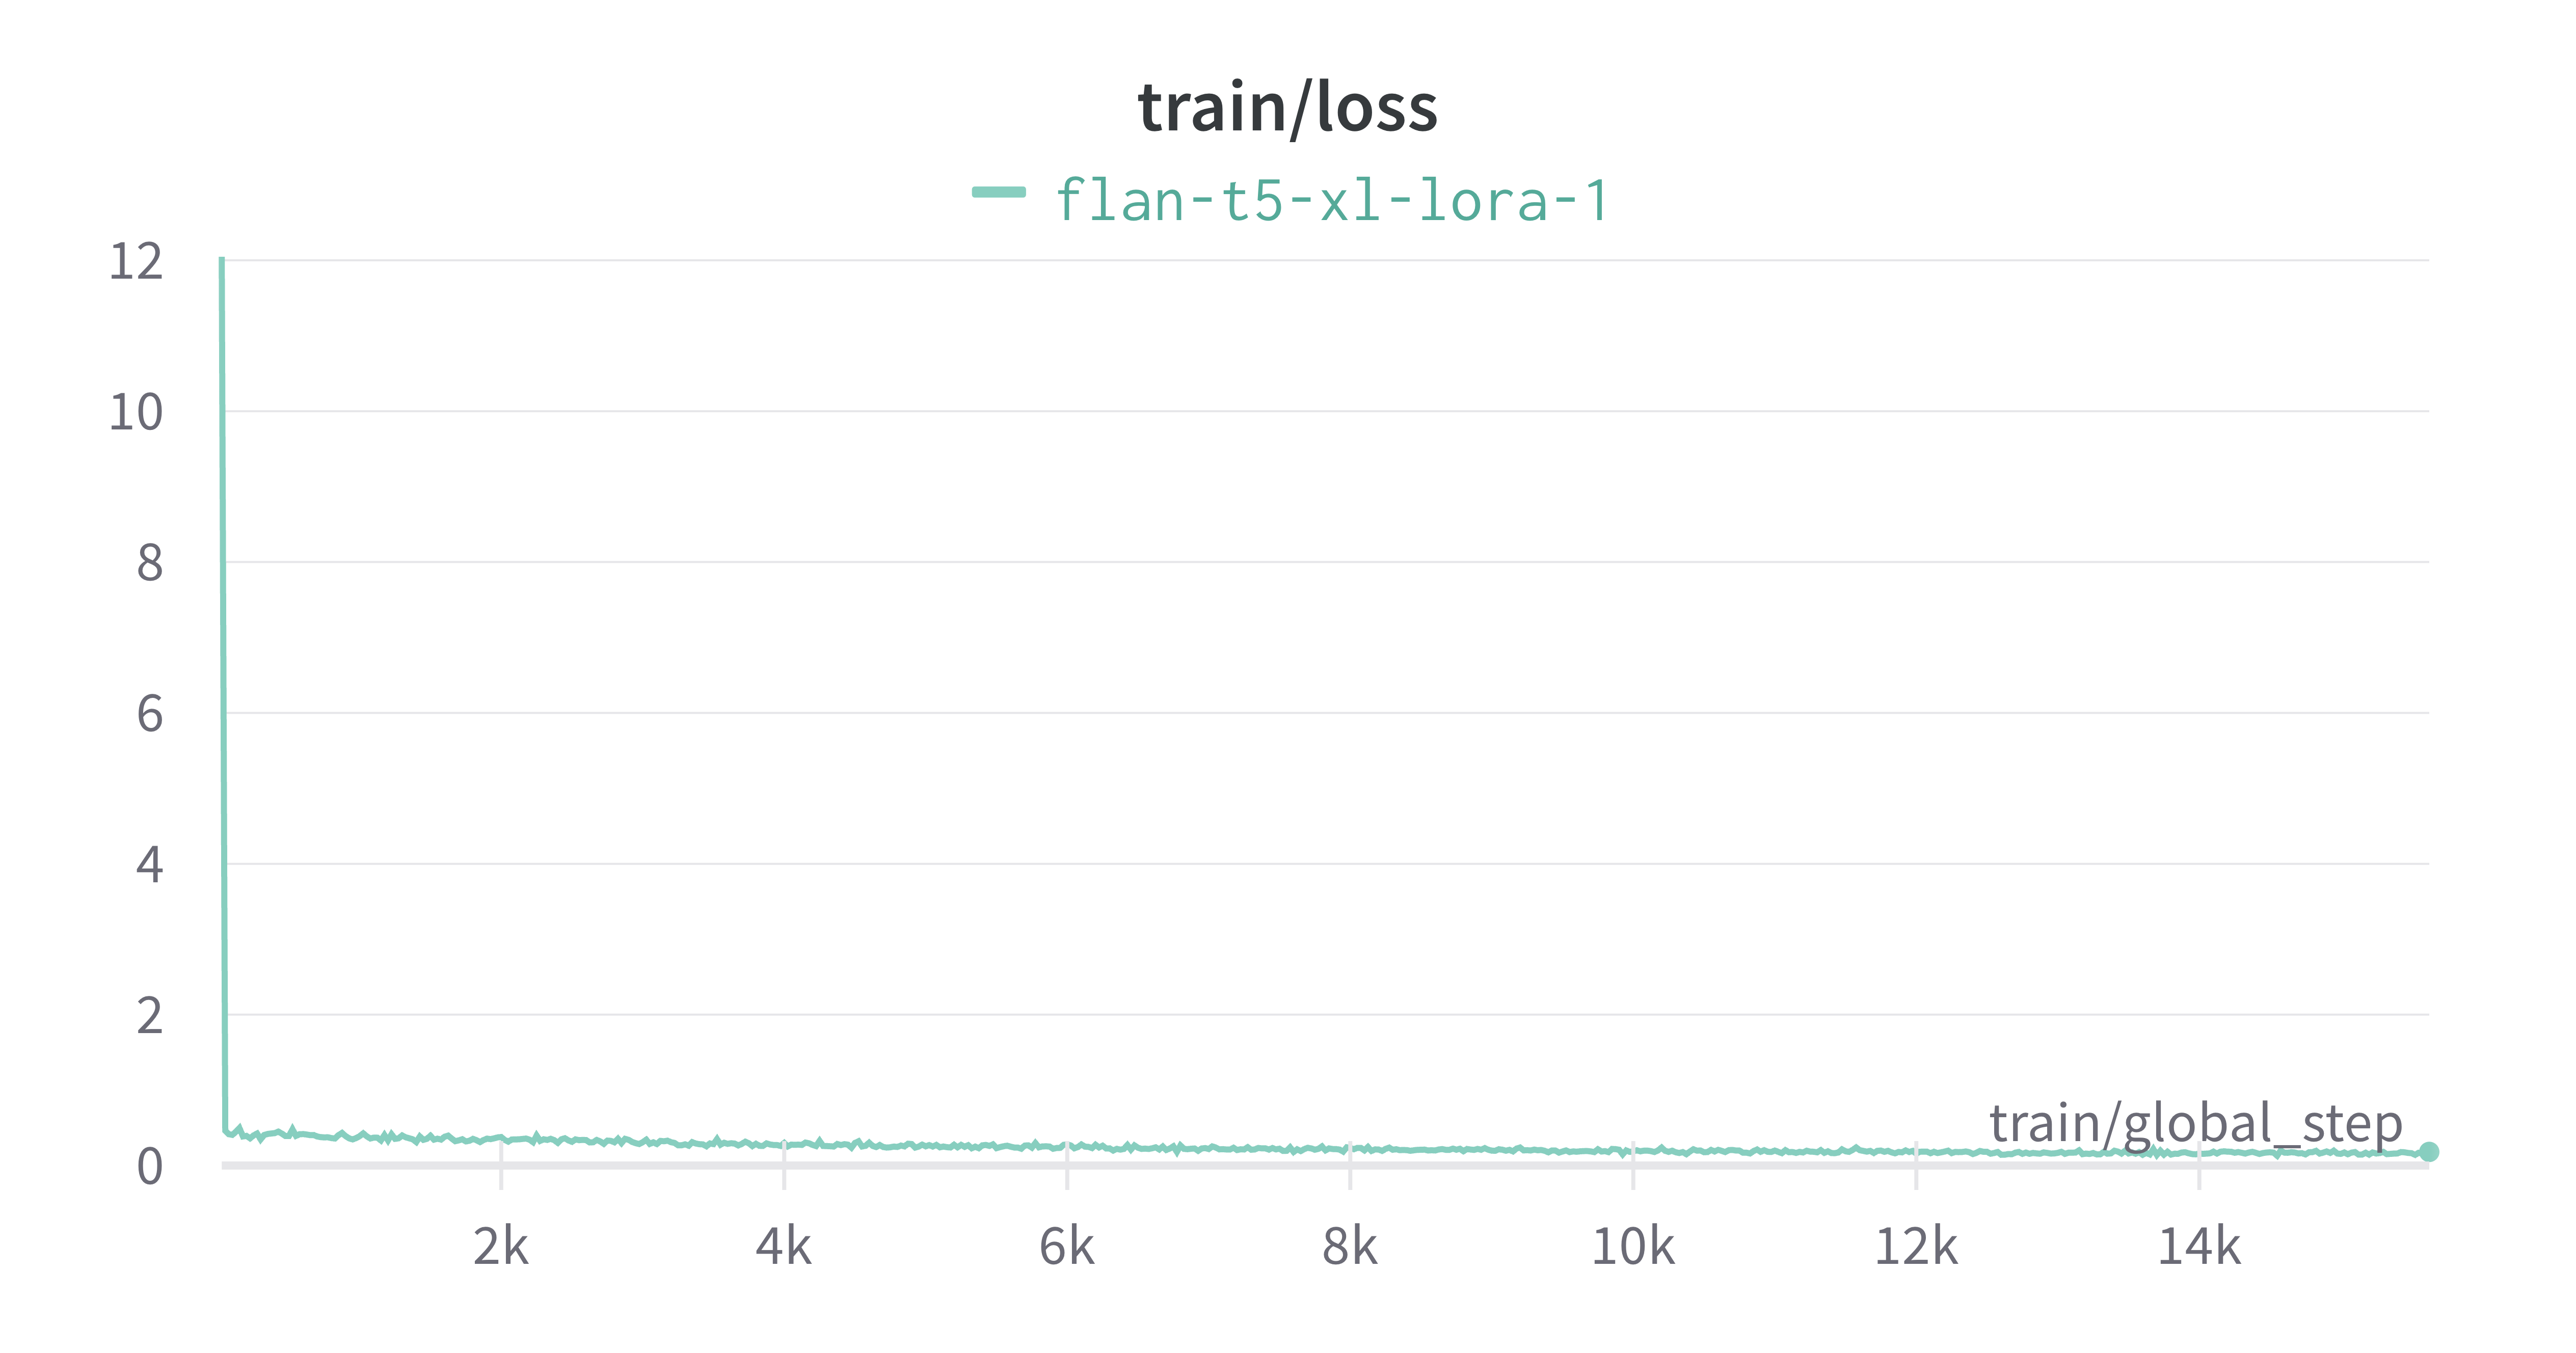
\includegraphics[width=.6\textwidth]{total-train-loss}
  \caption{Значение функции ошибки на тренировочных данных}
  \label{total-train-loss}
\end{figure}

\begin{figure}[H]
  \centering
  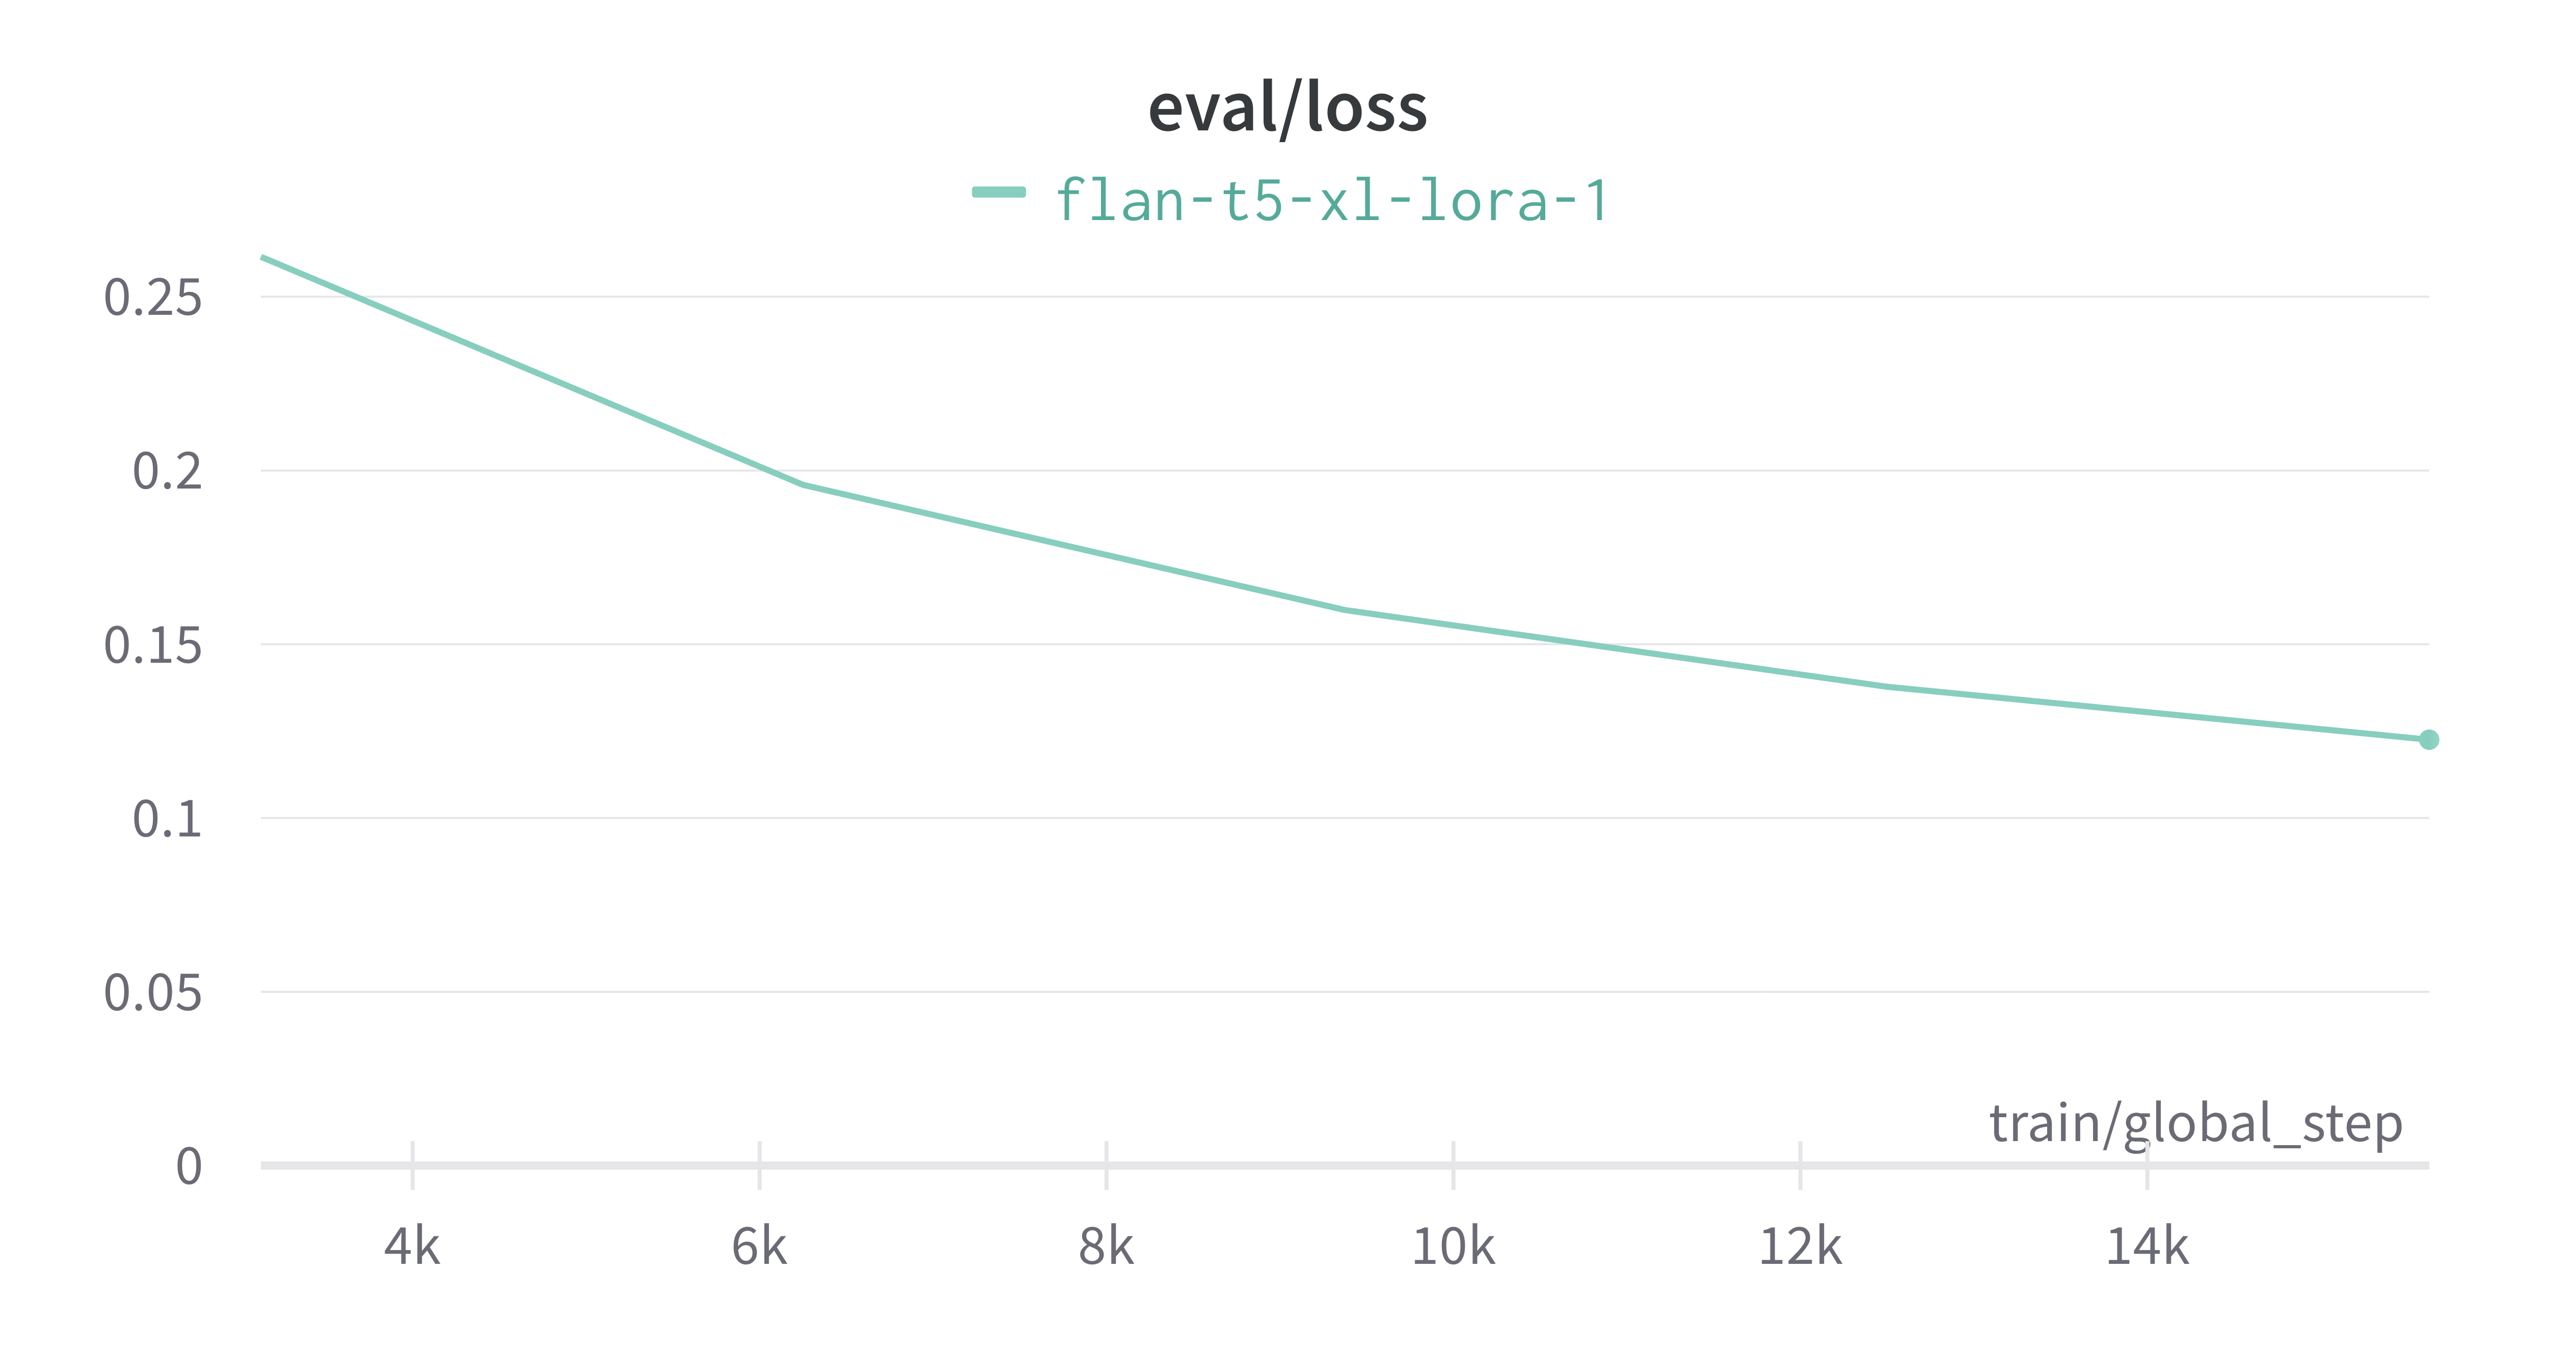
\includegraphics[width=.6\textwidth]{total-eval-loss}
  \caption{Значение функции ошибки на валидационных данных}
  \label{total-eval-loss}
\end{figure}

\begin{figure}[H]
  \centering
  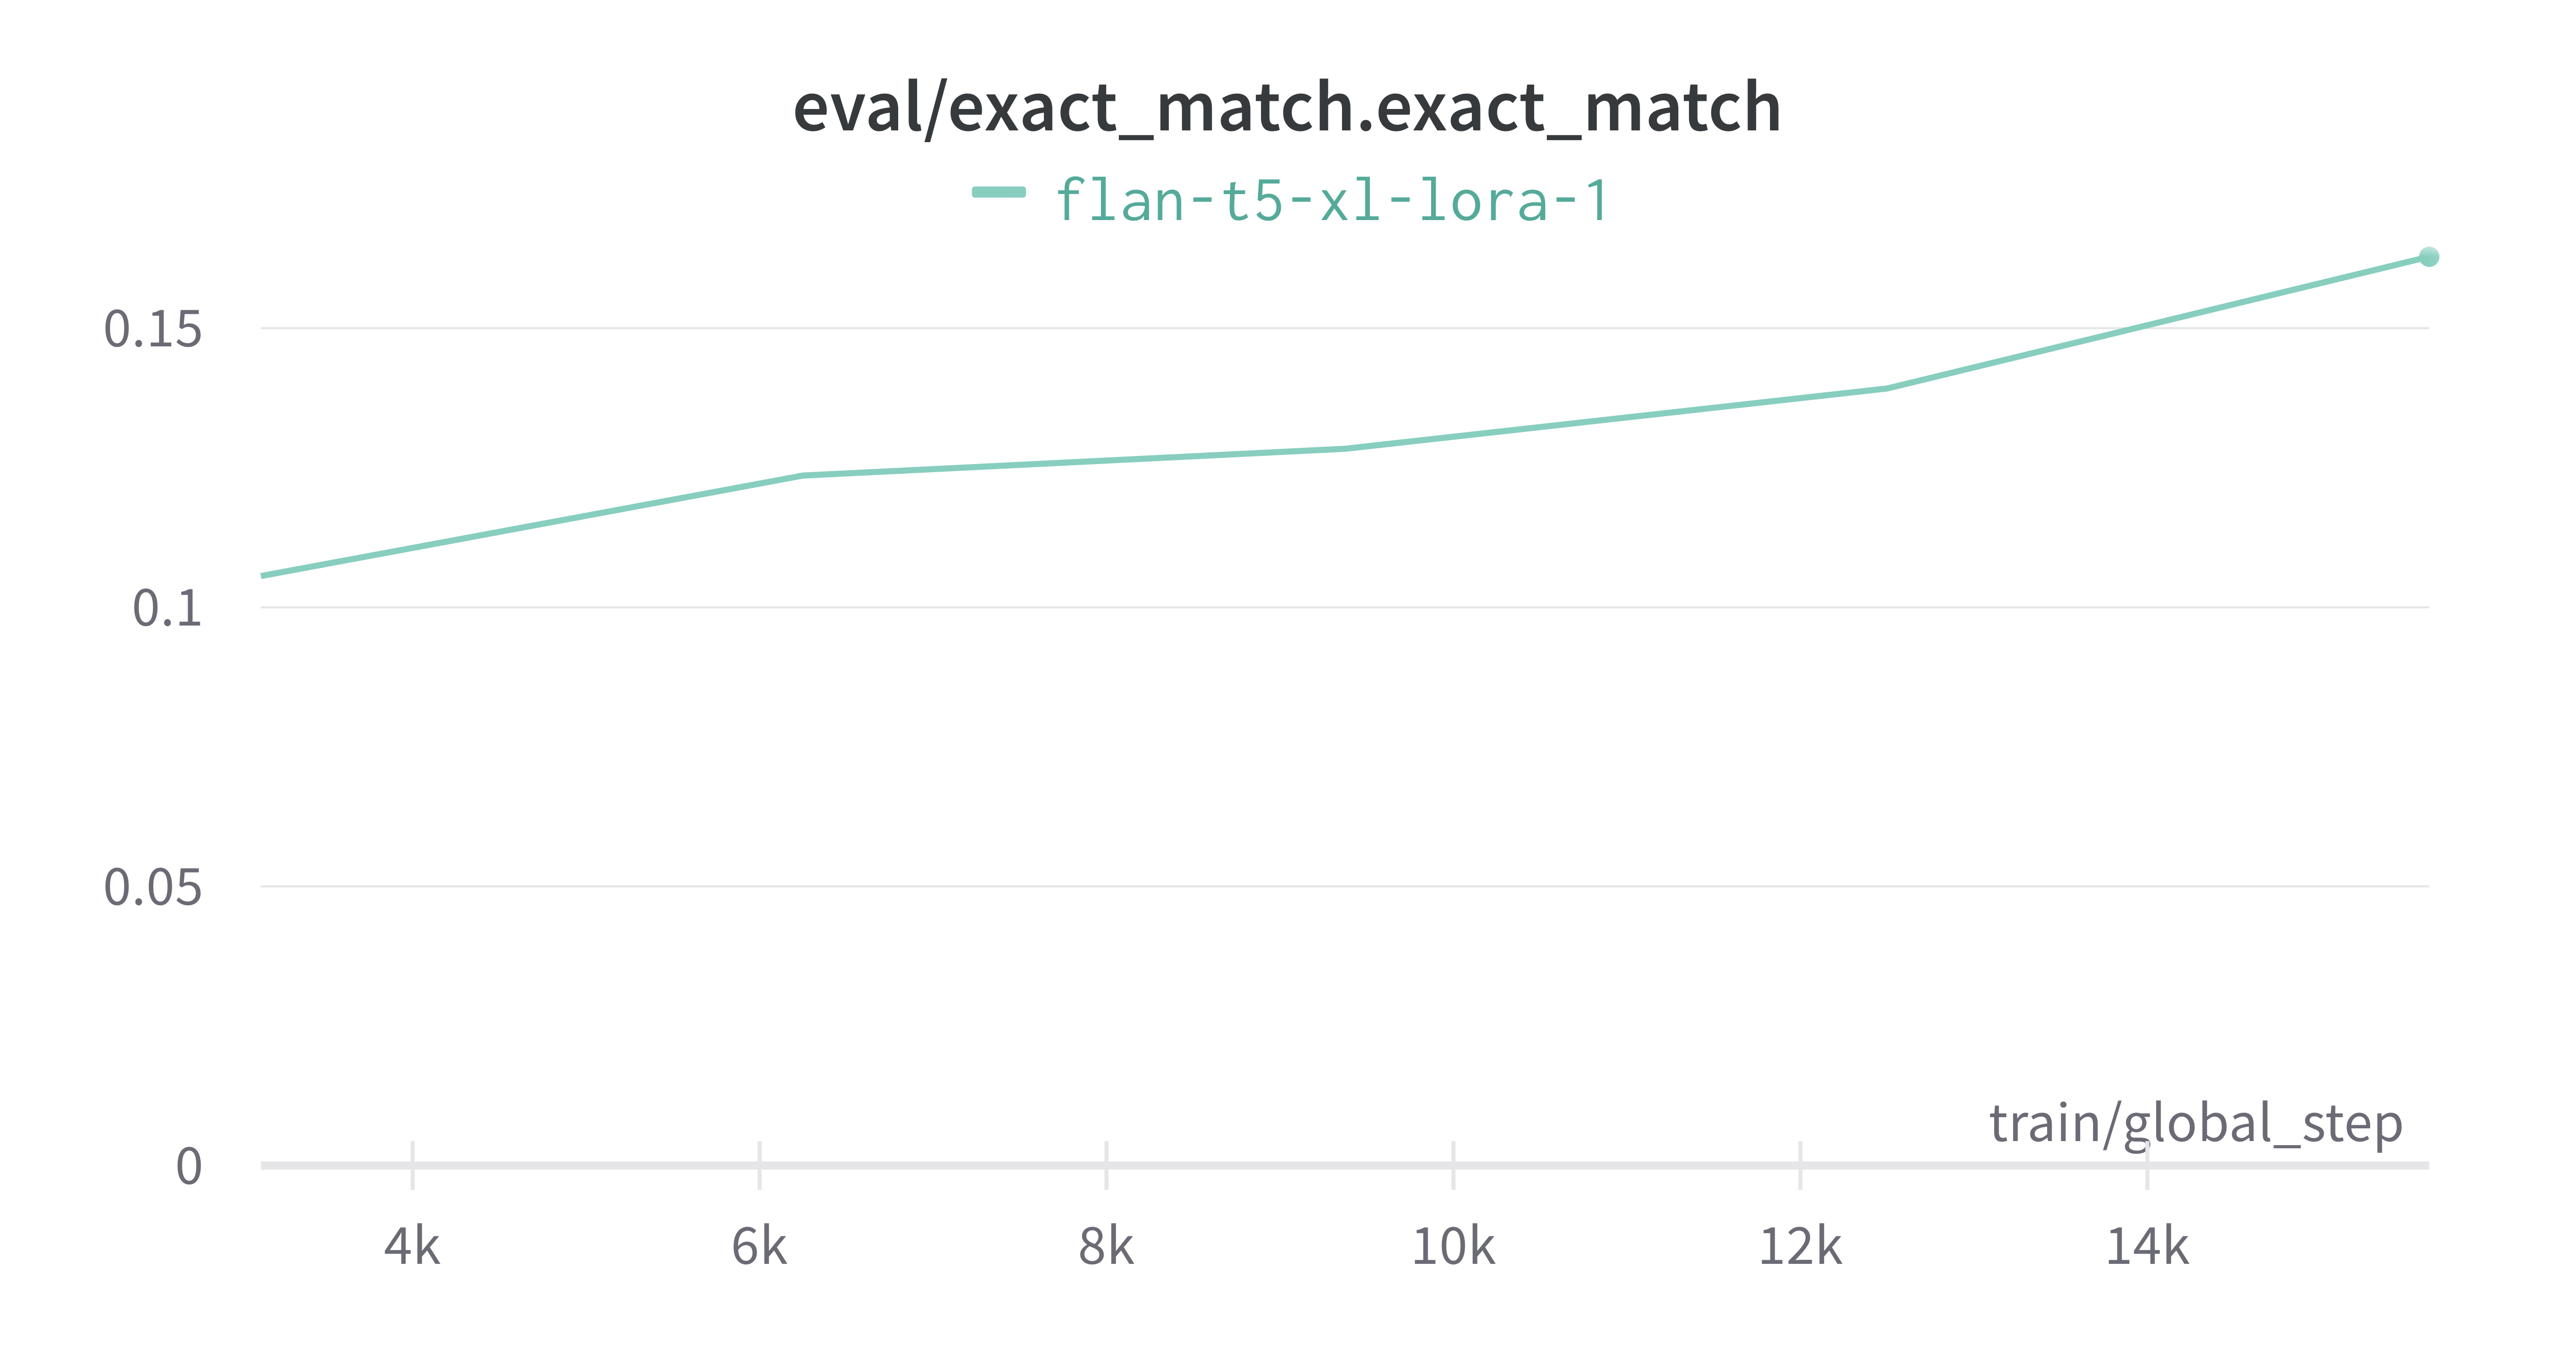
\includegraphics[width=.6\textwidth]{total-em}
  \caption{Значение метрики Exact Match на валидационных данных}
  \label{total-em}
\end{figure}

\begin{figure}[H]
  \centering
  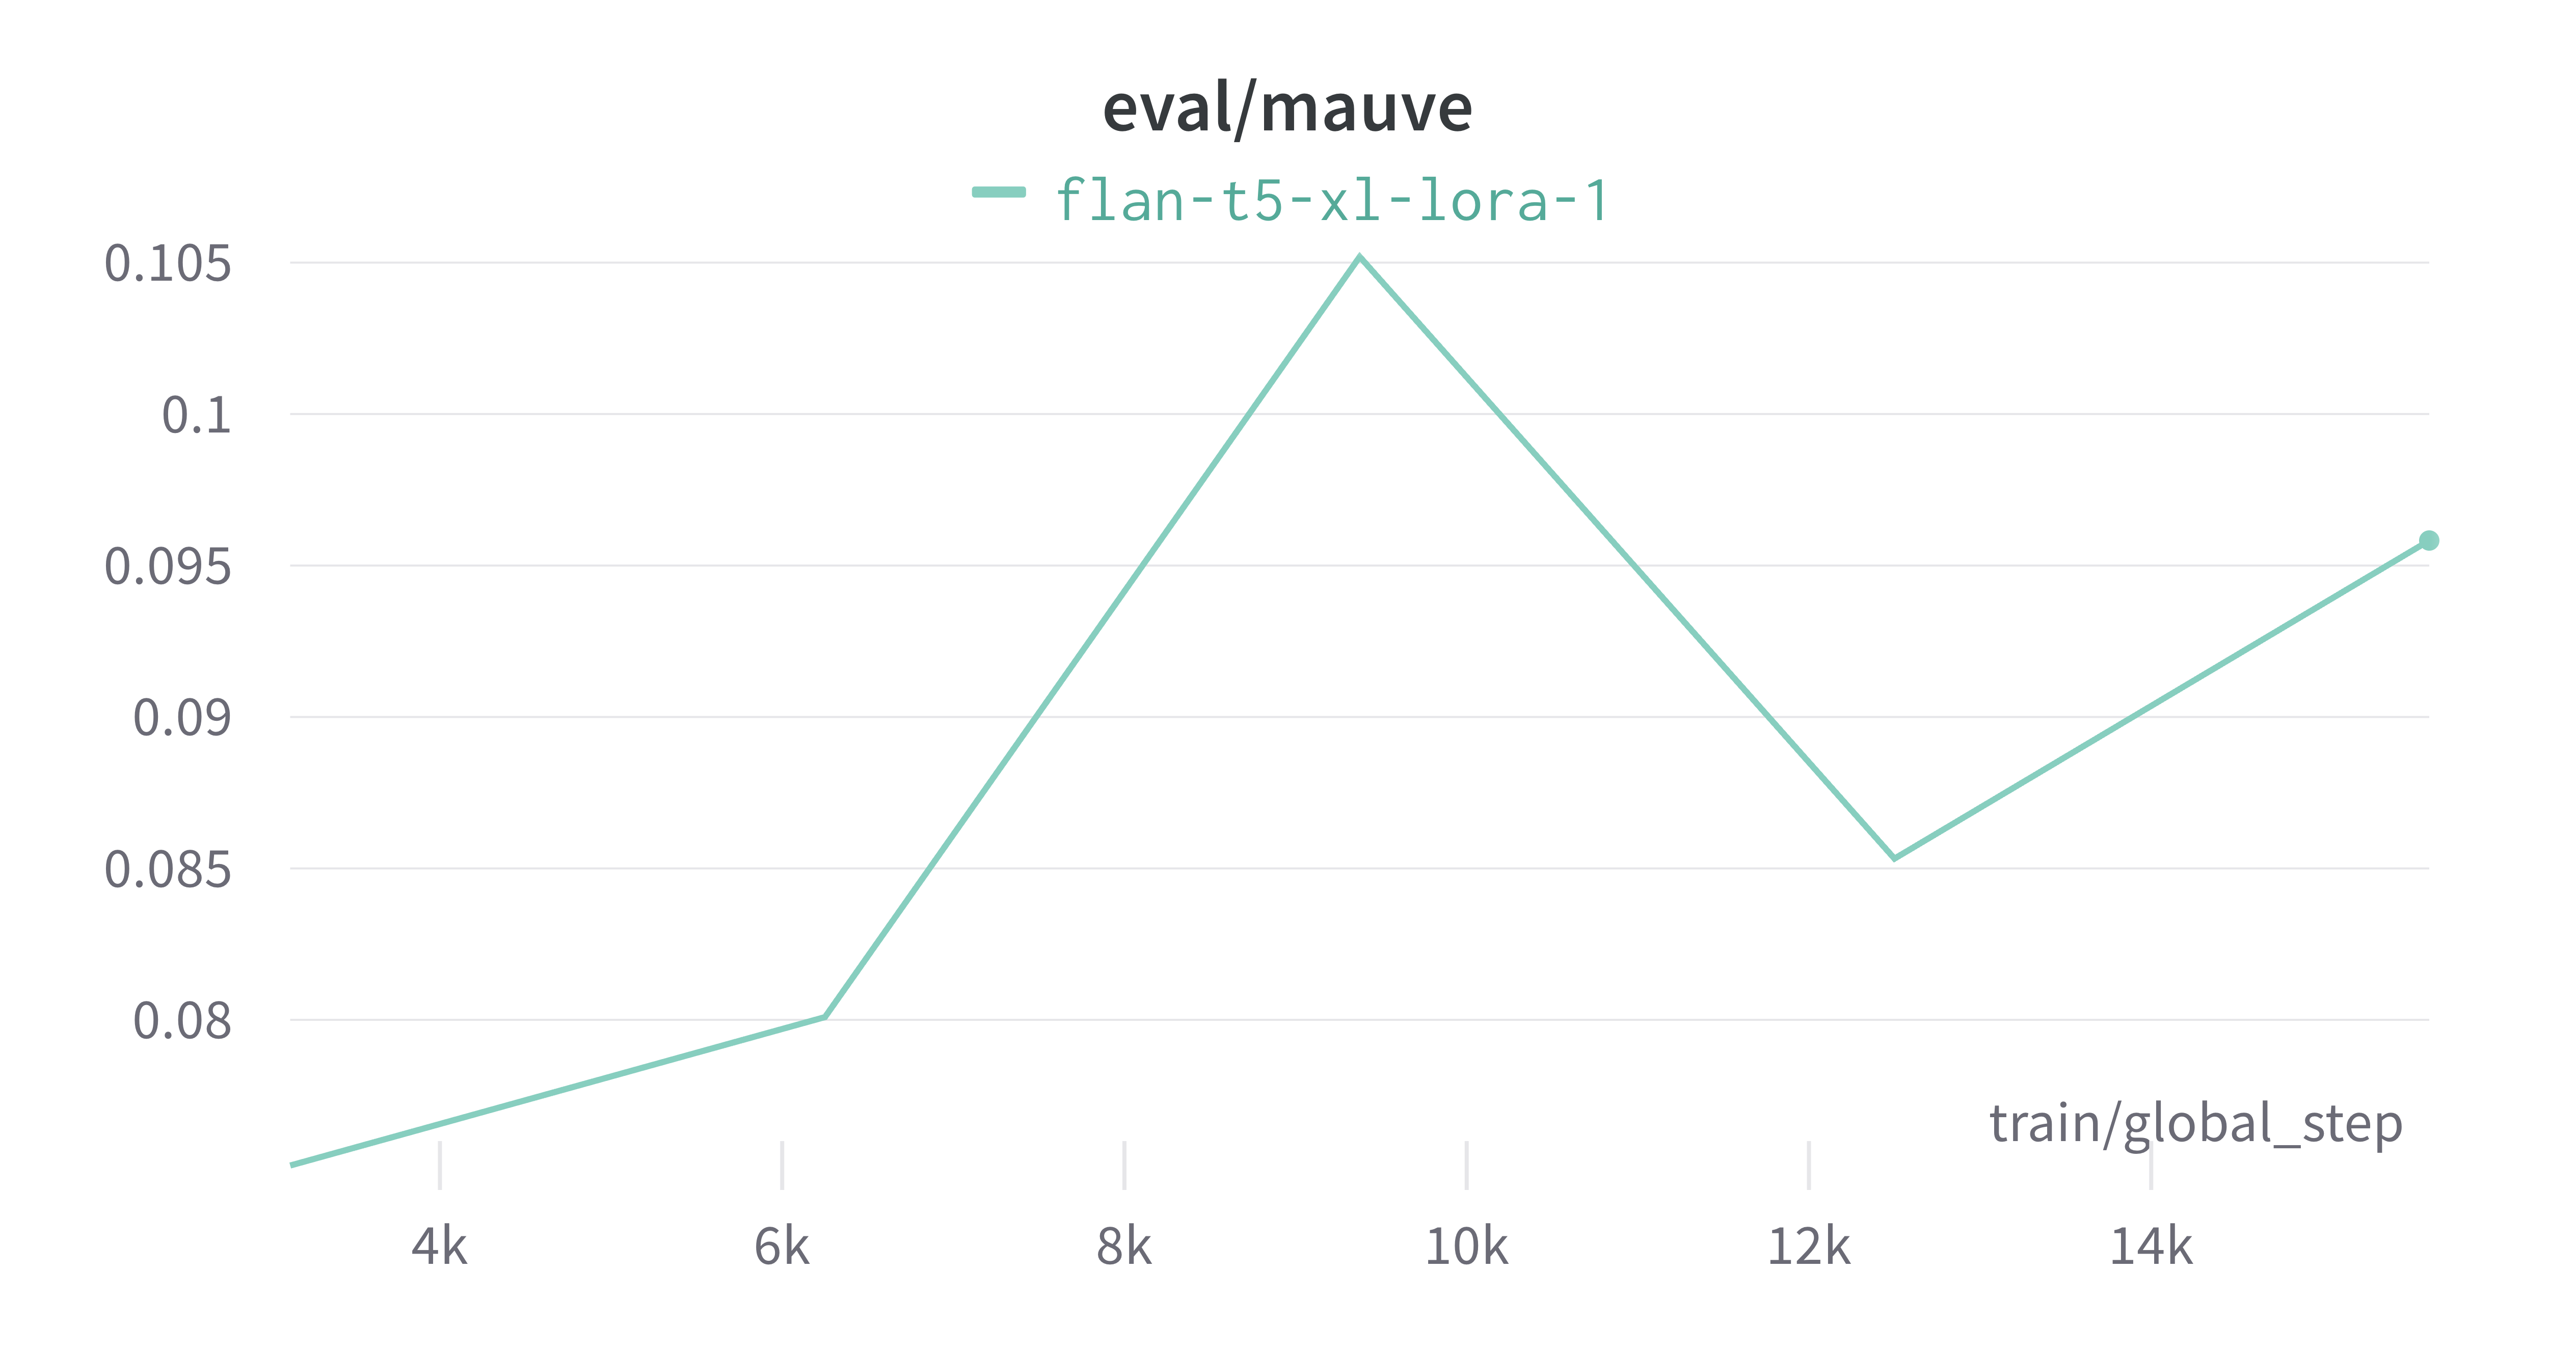
\includegraphics[width=.6\textwidth]{total-mauve}
  \caption{Значение метрики MAUVE на валидационных данных}
  \label{total-mauve}
\end{figure}


\chapter{ОПТИМИЗАЦИЯ МОДУЛЕЙ ИТОГОВОЙ СИСТЕМЫ}
После успешного обучения и тестирования на необходимых для решения задач данных модель ИНС используется на конечном устройстве: на сервере или на клиентском устройстве. Такое использование моделей ИНС называется инференсом модели ИНС. Во время инференса модель должна как можно более эффективно использовать ресурсы, т.к. это непосредственно сказывается на опыте использования приложений с использованием моделей ИНС.

При оптимизации моделей архитектуры трансформер важной задачей становится эффективное вычисление механизма внимания, т.к. это главный компонент такой архитектуры. Хоть механизм внимания и позволяет динамически учитывать контекст входных данных, но этот механизм не лишен недостатков. К недостаткам расчета внимания с точки зрения ускорительных расчетов относятся:
\begin{enumerate}
    \item Высокие требования к вычислениям и памяти. Вычисление внимания включает в себя большое количество матричных умножений и обращений к памяти, которые могут требовать значительных вычислительных ресурсов и памяти, особенно для больших входных последовательностей.
    \item Сложность распараллеливания. Последовательный характер расчета внимания затрудняет эффективное распараллеливание между несколькими ядрами или графическими процессорами. Это может привести к неэффективному использованию аппаратных ресурсов и увеличению времени обработки.
    \item Ограниченная масштабируемость модели. Высокие требования к вычислительным ресурсам и памяти для расчета внимания могут ограничивать масштабируемость моделей, использующих внимание, особенно для задач, включающих длинные входные последовательности или требующих карт объектов с высоким разрешением.
    \item Ограниченная поддержка аппаратных ускорителей. Существующие аппаратные ускорители могут быть не оптимизированы для конкретных вычислений, связанных с расчетом внимания, что приводит к неоптимальной производительности и энергопотреблению.
\end{enumerate}

Данные недостатки можно пробовать нивелировать путём аппроксимации вычислений механизма внимания, но в таком случае будет страдать качество обучаемых моделей. Механизм FlashAttention \cite{flash-attn-paper} эффективно вычисляет механизм внимания, при этом не являясь аппроксимацией.

Оптимизация FlashAttention заключается в более эффективном обращении к памяти ускорителя за счёт разделения вычислений на блоки, целиком размещаемые в наиболее быструю память ускорителя (на графических картах это SRAM), и перевычисления блоков для обратного распространения с целью снизить нагрузку на потребляемую память с $O(n^2)$ до $O(n)$.

\section{ОПТИМИЗАЦИЯ МОДУЛЯ КЛАССИФИКАЦИИ НАМЕРЕНИЙ}
Для оптимизации модуля классификации намерений было рассмотрено несколько подходов:
\begin{enumerate}
    \item Оптимизация Python кода. Такие виды оптимизаций нацелены на минимизацию затрат использования Python интерпретатора за счет компиляции программы. Примером может служить функция \texttt{torch.compile}, доступная во фреймворке PyTorch \cite{pt-docs}.
    \item Оптимизация алгоритмов вычисления. Примером такой оптимизации может быть использование механизма FlashAttention
    \item Оптимизация представления используемых типов данных. В качестве примера может выступать подход BetterTransformers, который использует разреженный тип матриц в блоках моделей архитектуры трансформер.
\end{enumerate}

Модуль классификации намерений как правило меньше и быстрее модуля диалоговой модели, поэтому тестирование различных видов оптимизаций проходило в условиях, когда эмулировалось множественное обращение к модели одновременно. Тестирование проходило посредством http запросов виртальных пользователей к серверу, обслуживающему модуль классификации. Из изменяемых параметров исследовалась зависимость пропускной способности и времени отклика от количества параллельно обрабатываемых запросов и различных оптимизаций. Тестирование различных видов оптимизаций проходило в два этапа:
\begin{enumerate}
    \item При достаточно сложных условиях с фиксированным количеством одновременно подключенных виртуальных пользователей (100).
    \item Второй этап проходил с нарастанием количества виртуальных пользователей.
\end{enumerate}

На рис. \ref{resp-time-1}, \ref{resp-time-1-speedup}, \ref{throughput-1-speedup} демонстрируется эффективность оптимизаций, таких как FlashAttention и BetterTransformers, которые значительно повышают производительность системы. При этом можно видеть, что при малом количестве параллельно обрабатываемых запросов FlashAttention производительнее BetterTransformers, но при количестве параллельно обрабатываемых запросов больше восьми BetterTransformers показывает производительность лучше. Такое поведение объясняется тем, что BetterTransformers улучшает производительность всей модели, тогда как FlashAttention оптимизирует только узкое горлышко модели. Использование обоих подходов позволит получить еще больше производительности.

\begin{figure}[H]
    \centering
    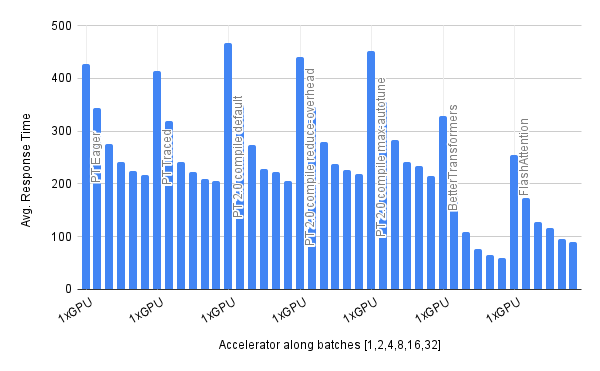
\includegraphics[width=.8\textwidth]{resp-time-1-test}
    \caption{График сравнения различных оптимизаций, количества параллельно обрабатываемых запросов с средним временем ответа сервера}
    \label{resp-time-1}
\end{figure}

\begin{figure}[H]
    \centering
    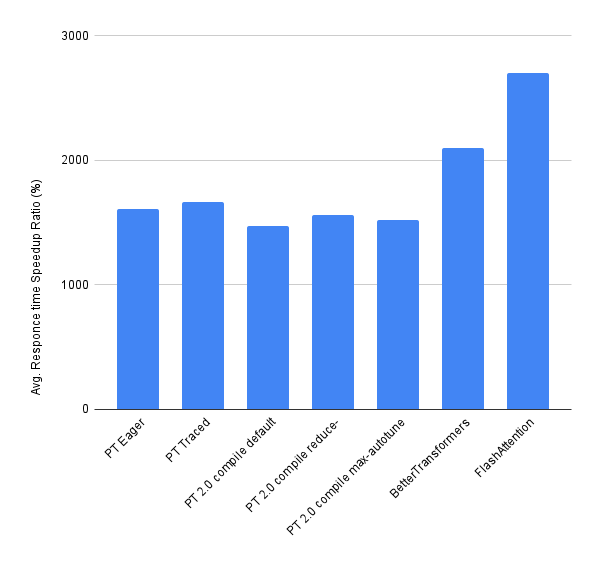
\includegraphics[width=.65\textwidth]{resp-speedup-1}
    \caption{ График сравнения различных оптимизаций с ускорением на среднем времени ответа сервера относительно запуска на процессоре}
    \label{resp-time-1-speedup}
\end{figure}

\begin{figure}[H]
    \centering
    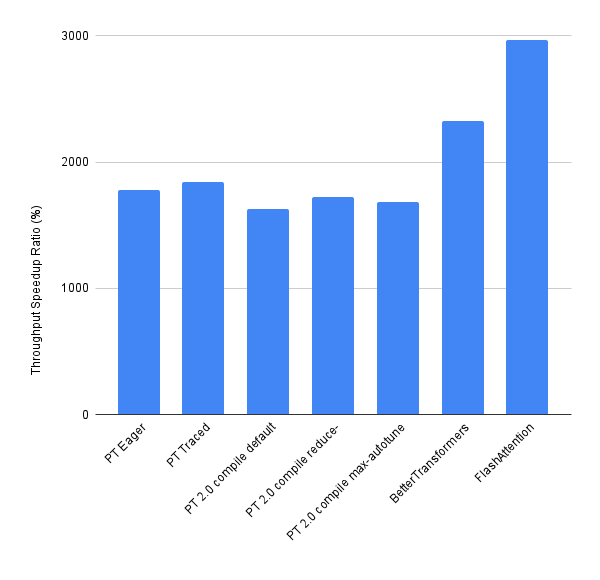
\includegraphics[width=.65\textwidth]{throughput-1-speedup}
    \caption{График сравнения различных оптимизаций с ускорением пропускной способности сервера относительно запуска на процессоре}
    \label{throughput-1-speedup}
\end{figure}

Тенденцию ускорения скорости обработки запросов модели за счет использование FlashAttention с нарастающим количеством виртальных пользователей можно наблюдать на рис. \ref{throughput-2}.

\begin{figure}[H]
    \centering
    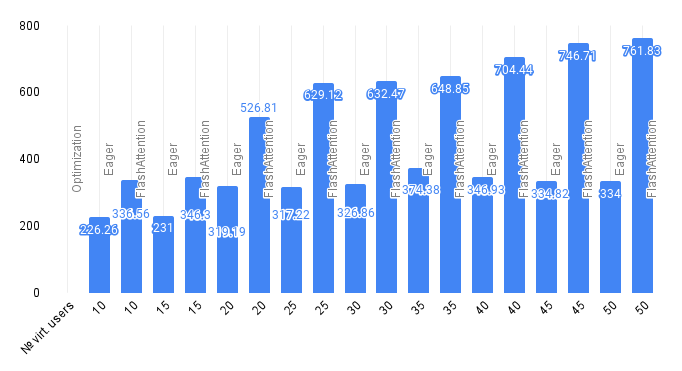
\includegraphics[width=.8\textwidth]{throughput-2}
    \caption{График сравнения пропускной способности сервера от количества пользователей}
    \label{throughput-2}
\end{figure}

Также стоит заметить важную деталь. Благодаря линейному росту зависимости потребляемой памяти у FlashAttention мы можем наблюдать, что FlashAttention заметно меньше потребляет видеопамять.

\begin{figure}[H]
    \centering
    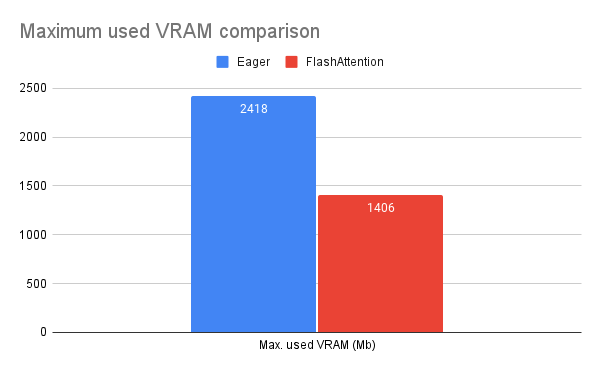
\includegraphics[width=.8\textwidth]{vram-clf}
    \caption{График сравнения максимально потребляемой видеопамяти от оптимизаций}
    \label{vram-clf}
\end{figure}

\section{ОПТИМИЗАЦИЯ МОДУЛЯ ДИАЛОГОВОЙ МОДЕЛИ}
Оптимизация скорости и количества потребляемых ресурсов модуля диалоговой модели является важным компонентом при разработке системы создания диалоговых агентов. Обычно модули диалоговой модели являются самой большой частью таких систем по части количества используемых вычислительных ресурсов. Помимо скорости обработки запросов моделью, важным компонентом становится количество потребляемой видеопамяти графической карты. Оптимизация по количеству потребляемой памяти позволит использовать диалоговую систему на клиентском устройстве, без необходимости обслуживать систему на сервере, хотя все еще требует иметь передовую потребительскую видеокарту (от NVIDIA GeForce RTX 3060 с видеопамятью 12Гб и выше). Примером технологии, благодаря которой можно значительно снизить количество потребляемой видеопамяти, можно назвать квантование.

Квантование -- это техника снижения затрат на вычисления и память при выполнении выводов путем представления весов и активаций низкоточными типами данных, такими как 8-битное целое число (int8) или 4-битное число вместо обычного 32-битного числа с плавающей точкой (float32). Это позволяет запускать модели даже на тех устройствах, которые поддерживают только целочисленные типы данных.

Из-за того, что модель Flan-T5 несовместима с использованием BetterTransformers из-за внутренних особенностей реализации архитектуры, то оптимизация данной модели проводилась с использованием различного квантования и FlashAttention.

Полная генерация ответа на один запрос пользователя может занимать секунды, что может плачевно сказаться на опыте использования системой. Чтобы решить эту проблему, генерируемый ответ модели можно транслировать пользователю потокенно. Первый отклик пользователь получит быстро и по мере генерации сможет читать ответ, генерируемый моделью. Таким образом, скоростью обработки модели генерации можно считать количество генерируемых токенов в секунду. Результаты производительности модели в зависимости от типа используемого квантования и использования FlashAttention приведены на рис. \ref{speed-quant}. Количество потребляемой при этом памяти можно наблюдать на рис. \ref{vram-quant}.

\begin{figure}[H]
    \centering
    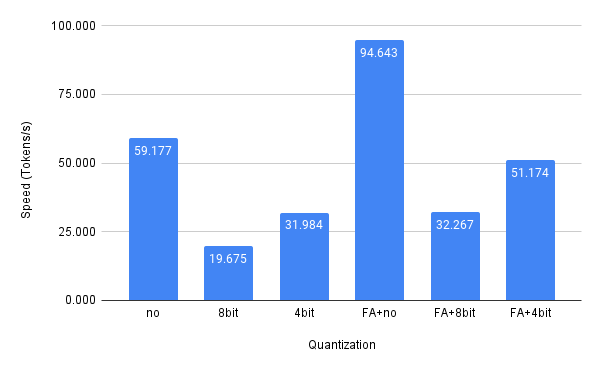
\includegraphics[width=.8\textwidth]{Speed_Quant}
    \caption{График сравнения скорости генерации от оптимизаций}
    \label{speed-quant}
\end{figure}

\begin{figure}[H]
    \centering
    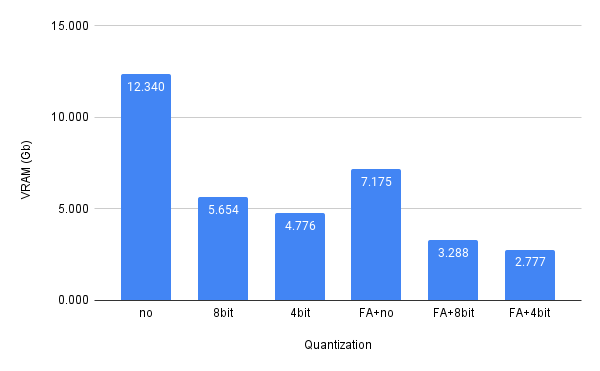
\includegraphics[width=.8\textwidth]{VRAM_Quant}
    \caption{График сравнения максимально потребляемой видеопамяти (Гб) от оптимизаций}
    \label{vram-quant}
\end{figure}

Скорость генерации при использовании модели в режиме 8 бит объясняется тем, что использование данного квантования на данный момент не оптимизировано для использования генеративными моделями.
\addchap{ЗАКЛЮЧЕНИЕ}
В рамках данного исследования была поставлена цель исследования использования генеративных нейросетевых моделей и разработки эффективной диалоговой модели, способной генерировать качественные ответы на основе образа неигрового персонажа и контекста диалога. Был использован и проанализирован специально созданный для исследования набор данных DNDD (Dungeon \& Dragons Dialogues). Также этот набор данных подготовлен специально для эмуляции диалогов в играх. В процессе исследования был изучен метод обучения моделей искусственных нейронных сетей с учителем, архитектура трансформер и было исследовано влияние различных параметров, таких как скорость обучения и планировщик скорости обучения на процесс обучения.

На основе проведенных экспериментов можно сделать вывод о наилучшем выборе параметров для обучения модели. Для модели Flan-T5 был выявлен оптимальный планировщик скорости обучения -- константный планировщик, а оптимальное значение скорости обучения составляет $9 \times 10^{-4}$. Это сочетание показало лучшие результаты по функциям ошибок и метрикам на представленных наборах данных.

В целом, полученные результаты демонстрируют возможность обучения эффективной диалоговой модели на доступных вычислительных ресурсах. Дальнейшие исследования и улучшения в области диалоговых моделей могут привести к еще более точным и качественным результатам.
\break

\begin{thebibliography}{99}
  \addcontentsline{toc}{chapter}{СПИСОК ЛИТЕРАТУРЫ}
  \bibitem{human-wer}
  Lippmann R. P. Speech recognition by machines and humans [Текст] // Speech communication. – 1997. – Т. 22. – №. 1. – С. 1-15.
  \bibitem{whisper}
  Radford A. et al. Robust speech recognition via large-scale weak supervision [Текст] // arXiv preprint arXiv:2212.04356. – 2022.
  \bibitem{state-of-gpt}
  Karpathy A. State of GPT [Электронный ресурс]. --- URL: \url{https://karpathy.ai/stateofgpt.pdf} (дата обр. 11.06.2023)
  \bibitem{transformer-paper}
  Vaswani A. et al. Attention is all you need [Текст] // Advances in neural information processing systems. – 2017. – Т. 30.
  \bibitem{backprop-theory}
  Hecht-Nielsen R. Theory of the backpropagation neural network [Текст] // Neural networks for perception. – Academic Press, 1992. – С. 65-93.
  \bibitem{optimizers-paper}
  Ruder S. An overview of gradient descent optimization algorithms [Текст] // arXiv preprint arXiv:1609.04747. – 2016.
  \bibitem{adafactor-paper}
  Shazeer N., Stern M. Adafactor: Adaptive learning rates with sublinear memory cost [Текст] // International Conference on Machine Learning. – PMLR, 2018. – С. 4596-4604.
  \bibitem{word2vec-paper}
  Mikolov T. et al. Efficient estimation of word representations in vector space [Текст] // arXiv preprint arXiv:1301.3781. – 2013.
  \bibitem{bpe-paper}
  Sennrich R., Haddow B., Birch A. Neural machine translation of rare words with subword units [Текст] // arXiv preprint arXiv:1508.07909. – 2015.
  \bibitem{gpt-paper}
  Radford A. et al. Improving language understanding by generative pre-training. – 2018.
  \bibitem{t5-paper}
  Raffel C. et al. Exploring the limits of transfer learning with a unified text-to-text transformer [Текст] // The Journal of Machine Learning Research. – 2020. – Т. 21. – №. 1. – С. 5485-5551.
  \bibitem{bert-paper}
  Devlin J. et al. Bert: Pre-training of deep bidirectional transformers for language understanding [Текст] // arXiv preprint arXiv:1810.04805. – 2018.
  \bibitem{sentencepiece-paper}
  Kudo T., Richardson J. Sentencepiece: A simple and language independent subword tokenizer and detokenizer for neural text processing [Текст] // arXiv preprint arXiv:1808.06226. – 2018.
  \bibitem{flan-paper}
  Chung H. W. et al. Scaling instruction-finetuned language models [Текст] // arXiv preprint arXiv:2210.11416. – 2022.
  \bibitem{weidu-repo}
  Репозиторий проекта WeiDU [Электронный ресурс]. --- URL: \url{https://github.com/WeiDUorg/weidu}
  \bibitem{llama-paper}
  Touvron H. et al. Llama: Open and efficient foundation language models [Текст] // arXiv preprint arXiv:2302.13971. – 2023.
  \bibitem{alpaca-docs}
  Документация Alpaca [Электронный ресурс]. --- URL: \url{https://crfm.stanford.edu/2023/03/13/alpaca.html} (дата обр. 06.06.2023)
  \bibitem{chatgpt-docs}
  Документация ChatGPT [Электронный ресурс]. --- URL: \url{https://openai.com/blog/chatgpt} (дата обр. 06.06.2023)
  \bibitem{MMLU-bench}
  Соревнование на наборе данных MMLU [Электронный ресурс]. --- URL: \url{https://paperswithcode.com/sota/multi-task-language-understanding-on-mmlu} (дата обр. 06.06.2023)
\end{thebibliography}

\appendix
\renewcommand{\thechapter}{\Asbuk{chapter}}
\chapter{ПРИМЕР ТРАНСЛЯЦИИ ИЗ ЯЗЫКА D В JSON}
\label{app:d2json}\texttt{\lstinputlisting[caption=$\text{Файл abishab.d}$]{./code/abishai.d}}
\texttt{\lstinputlisting[caption=$\text{Файл abishab.json}$]{./code/abishai.json}}
\chapter{ИСХОДНЫЙ КОД ОБРАБОТКИ DNDD}
\label{app:code}\texttt{\lstinputlisting[language={Python}, caption=$\text{Файл prepare.py}$]{./code/prepare.py}}
\texttt{\lstinputlisting[language={Python}, caption=$\text{Файл arg\_parser.py}$]{./code/arg_parser.py}}
\texttt{\lstinputlisting[language={Python}, caption=$\text{Файл descriptions.py}$]{./code/descriptions.py}}
\texttt{\lstinputlisting[language={Python}, caption=$\text{Файл dialogue\_data.py}$]{./code/dialogue_data.py}}
\texttt{\lstinputlisting[language={Python}, caption=$\text{Файл utils.py}$]{./code/utils.py}}

\chapter{ПРИМЕРЫ ДИАЛОГОВ}
\label{app:diagogue}\texttt{\lstinputlisting[language={}, caption=$\text{Пример диалога}$]{./code/diagogue.txt}}

\end{document}
